% BEGIN PREAMBEL
\documentclass[9pt]{beamer}
\usepackage[british]{babel}
\usepackage{multimedia}
\usepackage{amsmath,amsfonts,amssymb}
\usepackage{upgreek}
\usepackage{pgfpages}
\usepackage[version=3]{mhchem}
\usepackage{lmodern}
\usepackage{graphicx}
\usepackage{multicol}
\usepackage{color}
\usepackage{xcolor,fontawesome}
\usepackage{wrapfig}
\usepackage{siunitx}
\usepackage{fontspec}
\usepackage{tikz}
\usepackage{textpos}
\usepackage{booktabs}
\newfontfamily\ubuntu{Ubuntu}
\newcommand{\as}{\\[14pt]}
\newcommand{\s}{\\[7pt]}
\newcommand{\is}{\\[2pt]}
\newcommand{\no}{\noindent}
\newcommand{\ka}{\hspace*{0.5cm}}
\newcommand{\ma}{\hspace*{1cm}}
\newcommand{\ga}{\hspace*{1.5cm}}
\newcommand{\li}{\left|}
\newcommand{\re}{\right|}
\newcommand{\const}{\text{const.}}
\newcommand{\z}{\text}
\newcommand{\terminal}[1]{\colorbox{black}{\textcolor{white}{{\fontfamily{phv}\selectfont \scriptsize{#1}}}}}
\newcommand{\plugin}[1]{\textit{\flq#1\frq}}
\usetheme{Boadilla}
\graphicspath{ {Pics/} }
\usecolortheme{beaver}
\useoutertheme{miniframes}
\beamertemplatenavigationsymbolsempty
\makeindex
\title[Pad Performance]{Diamond pad detector performance at high rate at PSI}
\author[M. Reichmann]{Michael Reichmann}
\institute[\textbf{\textit{ETH}}\scalebox{.6}{\textit{Z\"{u}rich}}]{Swiss Federal Institute of Technology Zurich}
\AtBeginSection{\frame{\sectionpage}}
% END PREAMBEL
\begin{document}
% ============================
% BEGIN TITLE PAGE
% ============================
\usebackgroundtemplate{\tikz\node[opacity=0.2] {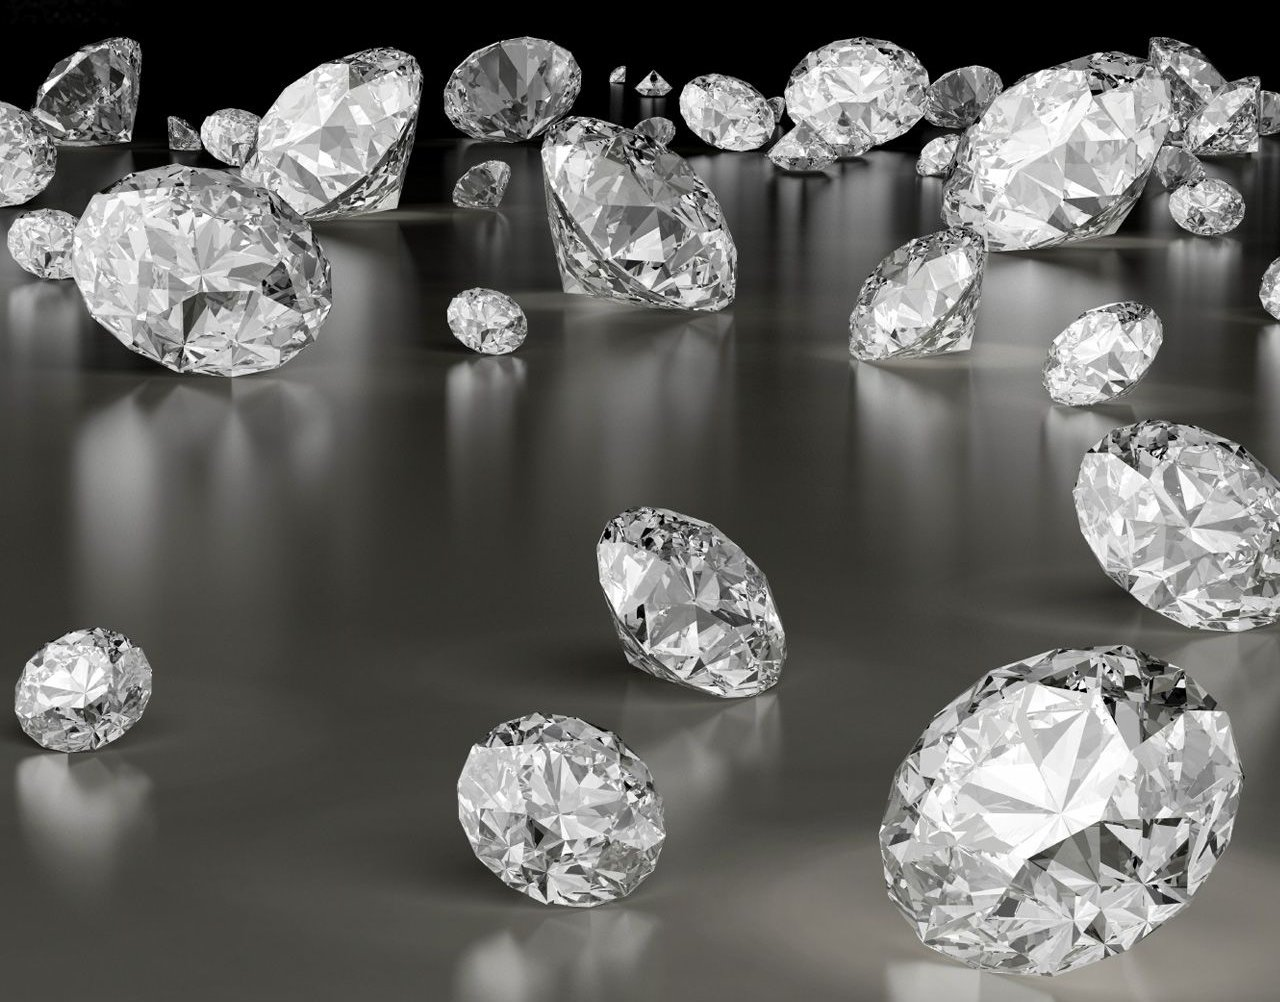
\includegraphics[height=\paperheight,width=\paperwidth]{bkg.jpg}};}
\begin{frame}
	\begin{center}
		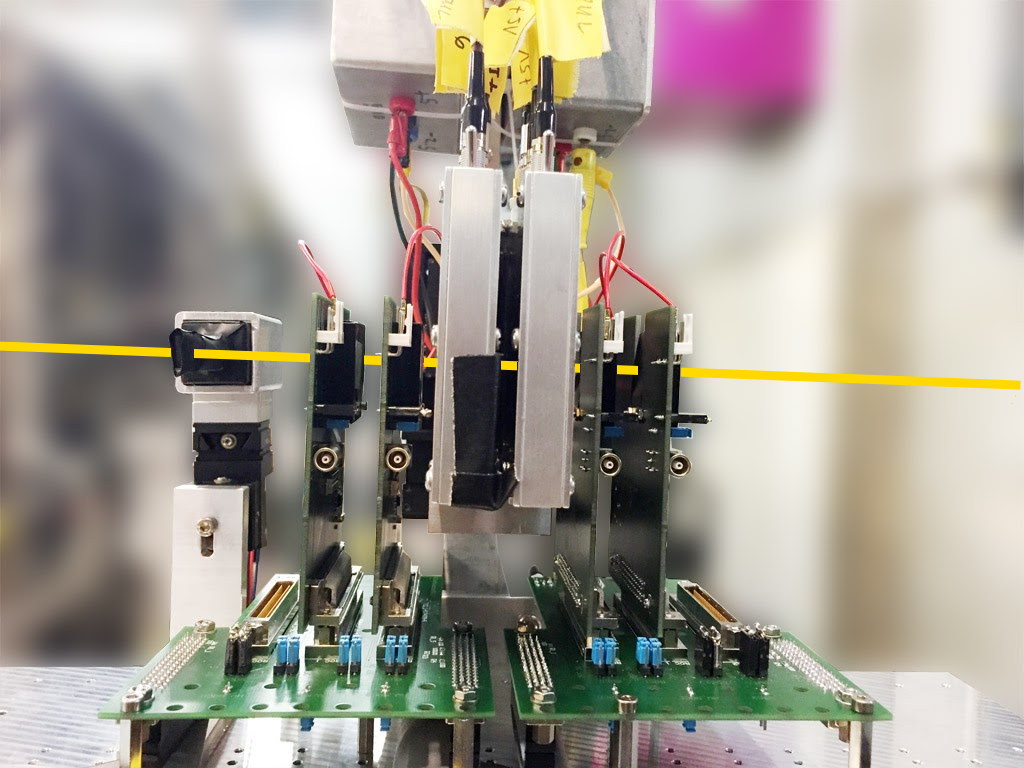
\includegraphics[width=6cm]{Setup1}
	\end{center}
	\begin{alertblock}{
		\begin{center}
			\textbf{Results of High Rate Tests of Diamond Pad Detectors at PSI}
		\end{center}}
		\vspace*{10pt}
		\begin{center}\small
		Michael Reichmann
		\end{center}\normalsize
	\end{alertblock}
\end{frame}
% END
\usebackgroundtemplate{}
% ============================
% BEGIN TABLE OF CONTENTS
% ============================
\begin{frame}[allowframebreaks]
	\frametitle{Table of contents}
	\tableofcontents   % [pausesections]
\end{frame}
% END
% ====================================================================================
% BEGIN INTRODUCTION
% ====================================================================================
\section{Introduction}
% ============================
\begin{frame}\
	\underline{\textbf{Goals of the beam test in August 2016:}}
	\begin{itemize}
		\setlength{\itemsep}{\fill}
		\item commissioning of the new setup ($\rightarrow$ Christians talk)
		\item confirming previous results $\rightarrow$ reproducibility
		\item investigating the high rate behaviour of higher irradiated diamonds
		\item testing a silicon diode as pad detector as reference
	\end{itemize}
	\vspace*{.3cm}
	\underline{\textbf{Measurements:}}
	\begin{itemize}
		\setlength{\itemsep}{\fill}
		\item tests of several diamond pad detectors and a silicon diode with a \SI{260}{Mev/c} pion beam at Paul Scherrer Institute (PSI)
		\item sizes:
		\begin{itemize}
			 \item diamonds $\approx$ \SI{5x5}{mm}
			 \item Si diode \SI{1.71x1.23}{mm}
		\end{itemize}
		\item irradiations: up to \SI[exponent-product = \cdot]{1e15}{neutrons/cm^{2}}
		\item diamond brands:
		\begin{itemize}
			\item Element Six (single and poly-crystal)
			\item II-IV Inc. (poly-crystal
		\end{itemize}
		\item flux range: from \SI{1}{kHz/cm^{2}} up to \SI{3}{MHz/cm^{2}} (at beam line pim1)
	\end{itemize}
\end{frame}
% new frame ==================
\begin{frame}
	\frametitle{Setup}
	\begin{center}
		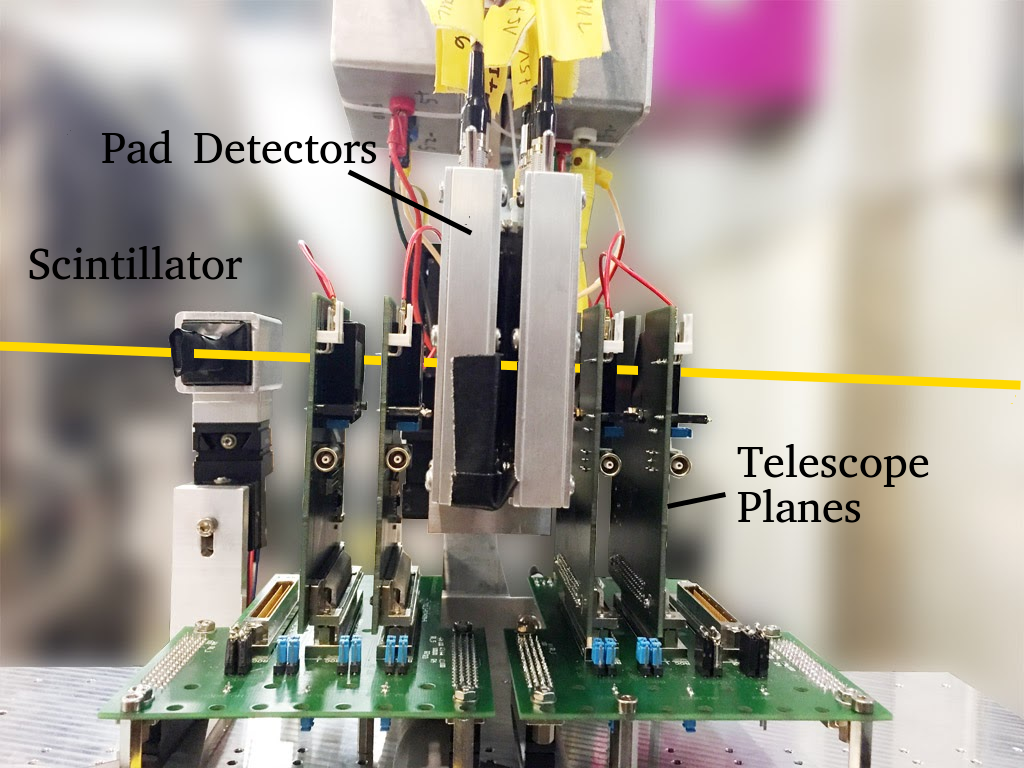
\includegraphics[width=6cm]{Setup}
	\end{center}
	\begin{itemize}
		\setlength{\itemsep}{\fill}
		\item 4 tracking planes with analogue CMS pixel chips
		\item 2 diamond pad detectors
		\item scintillator for precise trigger timing: sigma of \SI{1.3\pm.1}{ns}
% 		\item resolution: $\approx$ \SI{80x50}{$\upmu$m}
	\end{itemize}
\end{frame}
% new frame ==================
\begin{frame}
	\frametitle{Schematic Setup}
	\begin{center}
		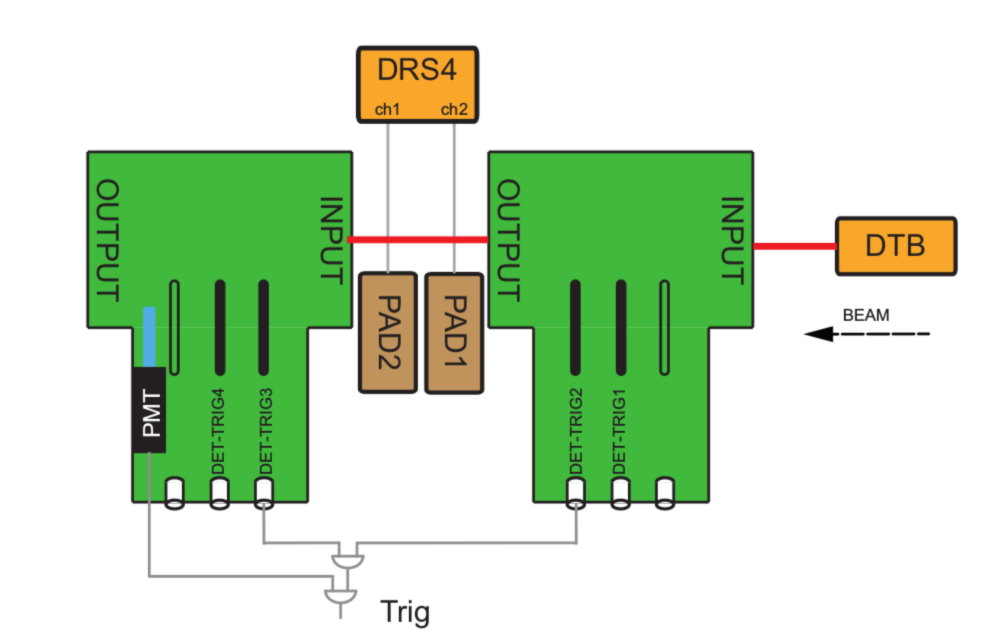
\includegraphics[width=7cm]{Schematics}
	\end{center}
	\begin{itemize}
		\setlength{\itemsep}{\fill}
		\item using PSI DRS4 Evaluation Board as digitizer for the pad waveforms
		\item using Digital Test Board (DTB) and pXar software for the telescope readout
		\item global trigger as coincidence of fastOR self trigger and scintillator signal
		\item EUDAQ as DAQ framework
	\end{itemize}
\end{frame}
% new frame ==================
\begin{frame}
	\frametitle{DAQ}
	\begin{center}
		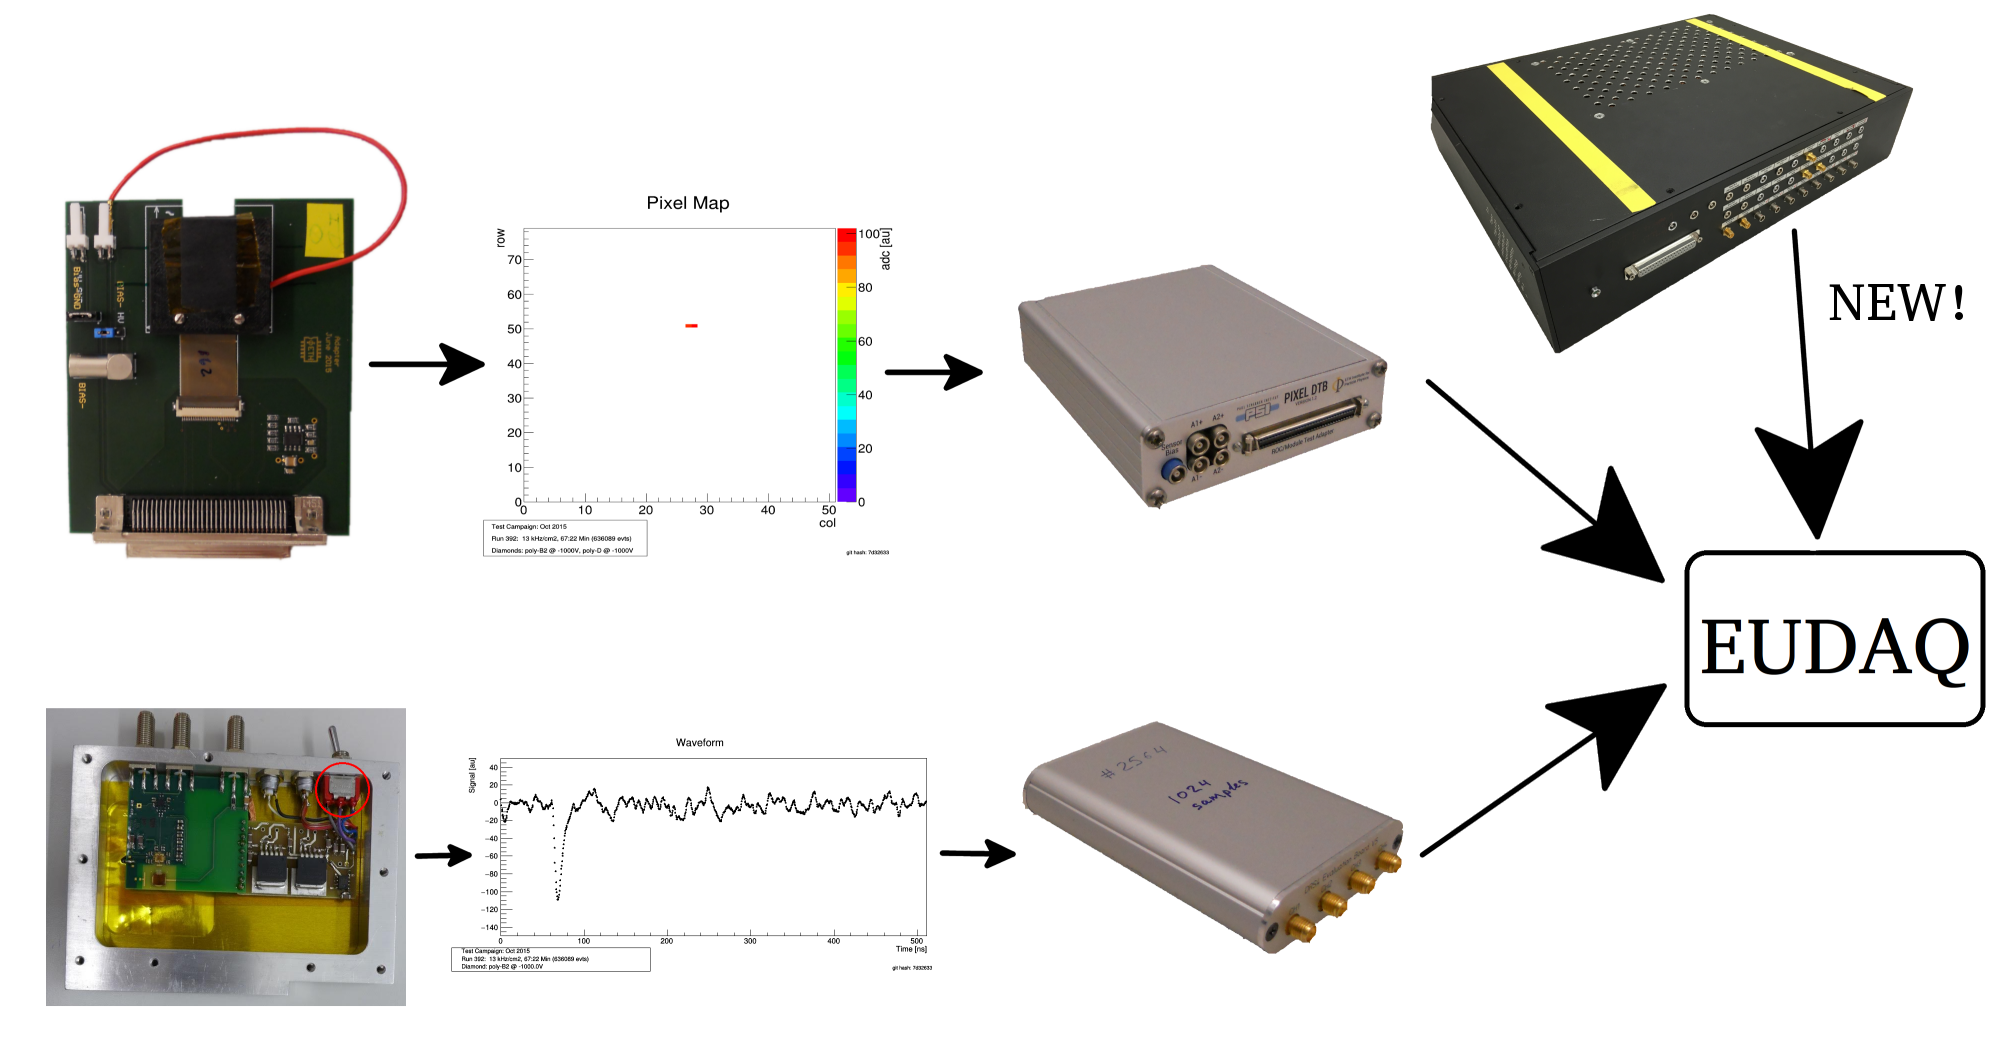
\includegraphics[width=.9\textwidth]{Intro}
	\end{center}
	\begin{itemize}
		\item EUDAQ saves event based data stream as binary file
		\item $\rightarrow$ conversion into ROOT-TTrees
	\end{itemize}
\end{frame}
% END
% ====================================================================================
% BEGIN ANALYSIS
% ====================================================================================
\section{Analysis}
% ============================
\subsection{Waveforms}
\begin{frame}
	\frametitle{Waveforms}
	\vspace*{-20pt}
	\begin{center}
		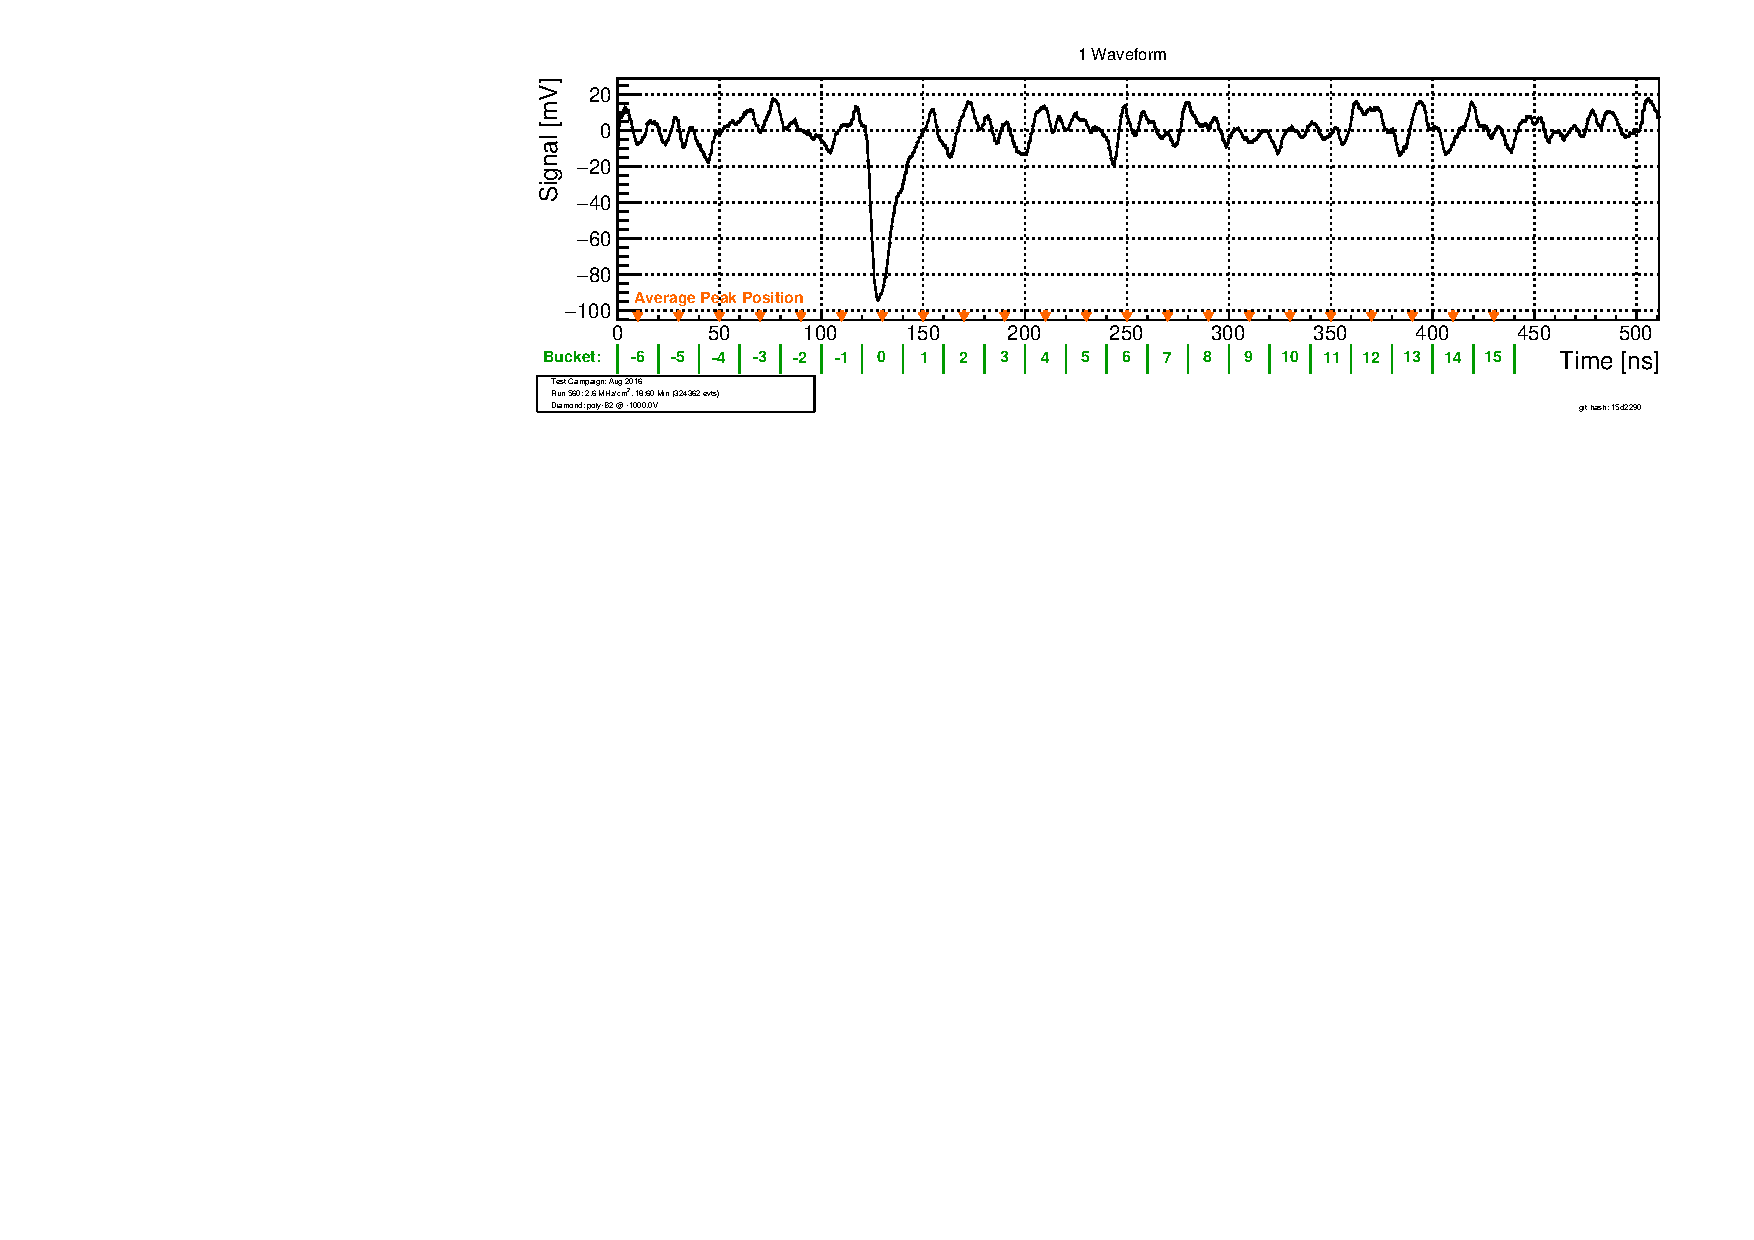
\includegraphics[angle=270, width=.7\textwidth]{SignalWaveform}\\
		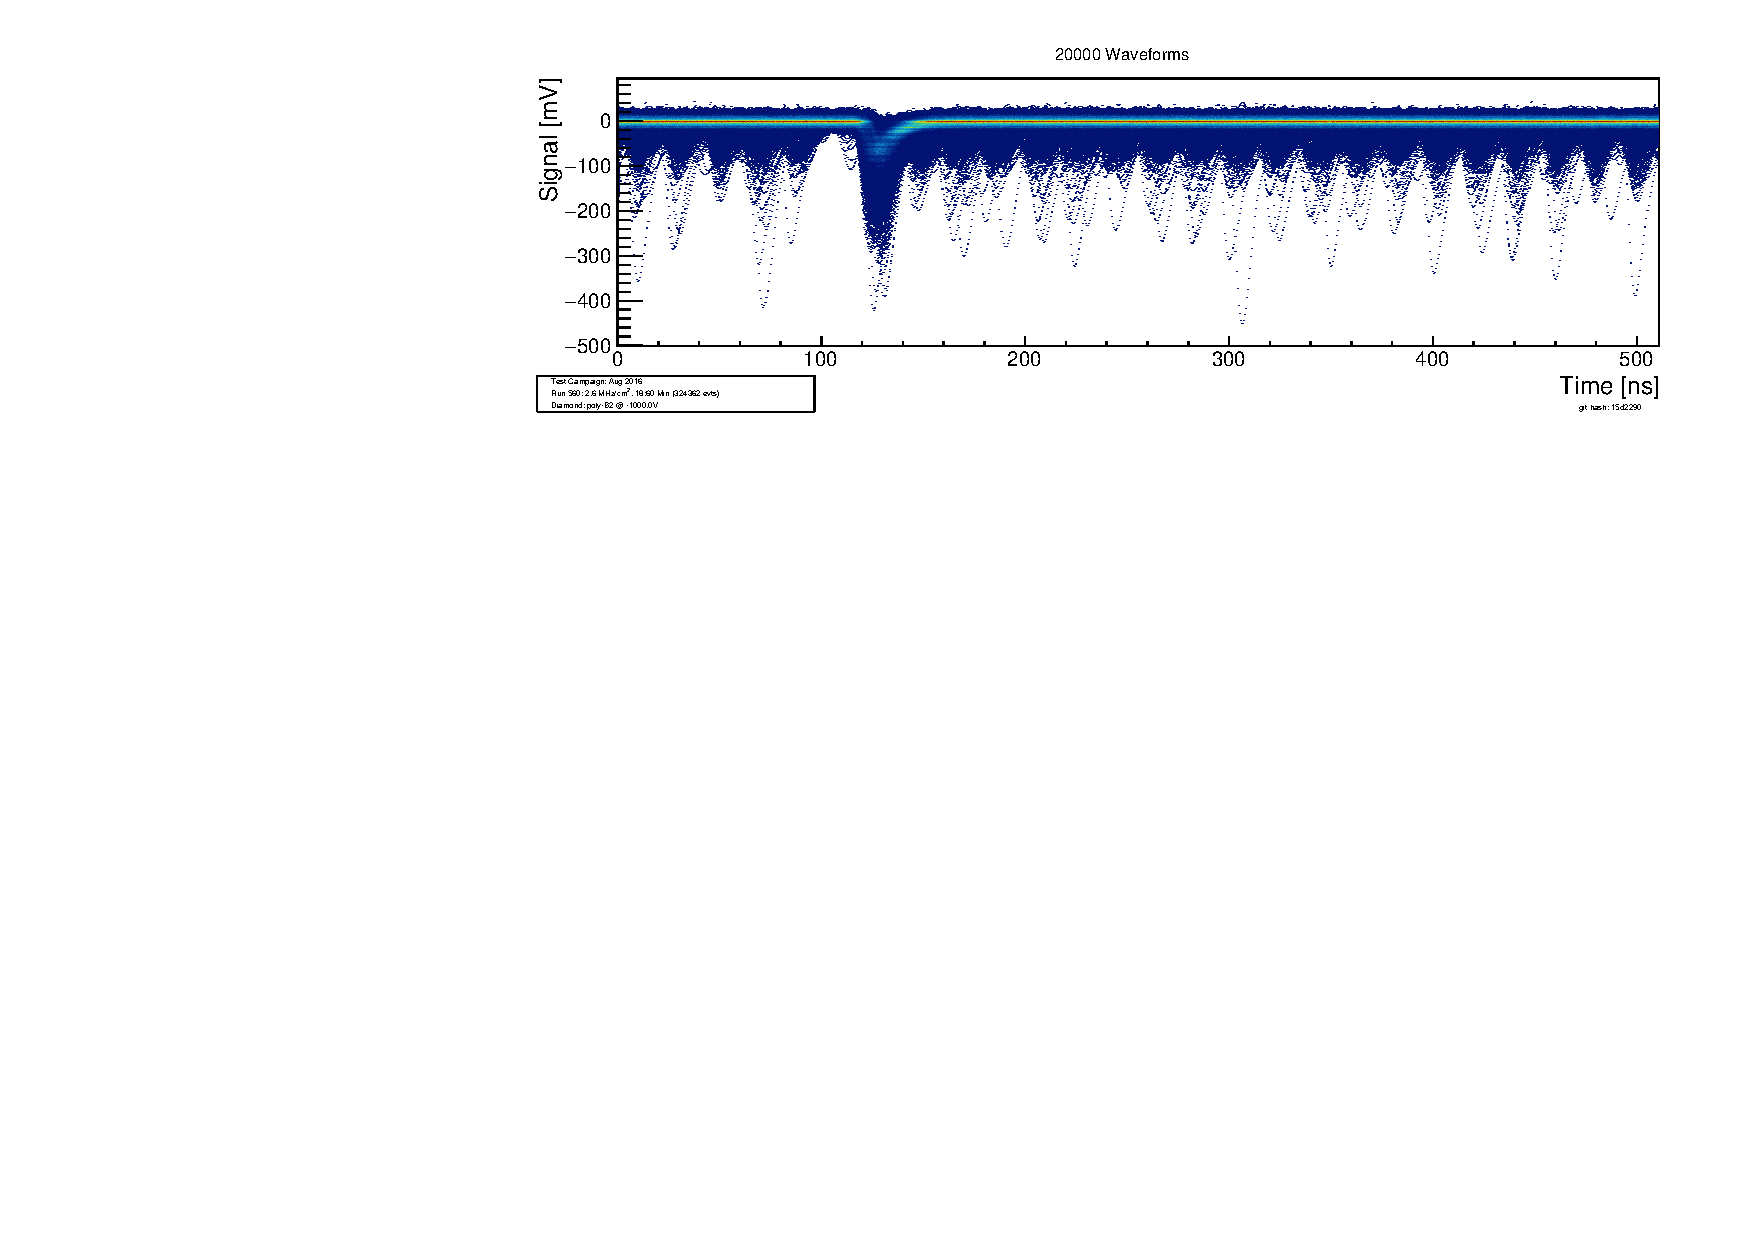
\includegraphics[angle=270, width=.7\textwidth]{SignalWaveforms20000}\\
	\end{center}
	\begin{itemize}
		\item most frequented peak (\SI{\approx130}{ns}): triggered signal
		\item other peaks originate from other buckets ($\rightarrow$ resolve beam structure of \SI{\approx19.7}{ns})
		\item system does not allow signals in pre-signal bucket due to fastOR trigger deadtime
	\end{itemize}
\end{frame}
% new frame =======================
\begin{frame}
	\frametitle{Pulse Height Calculation}
	\begin{center}
		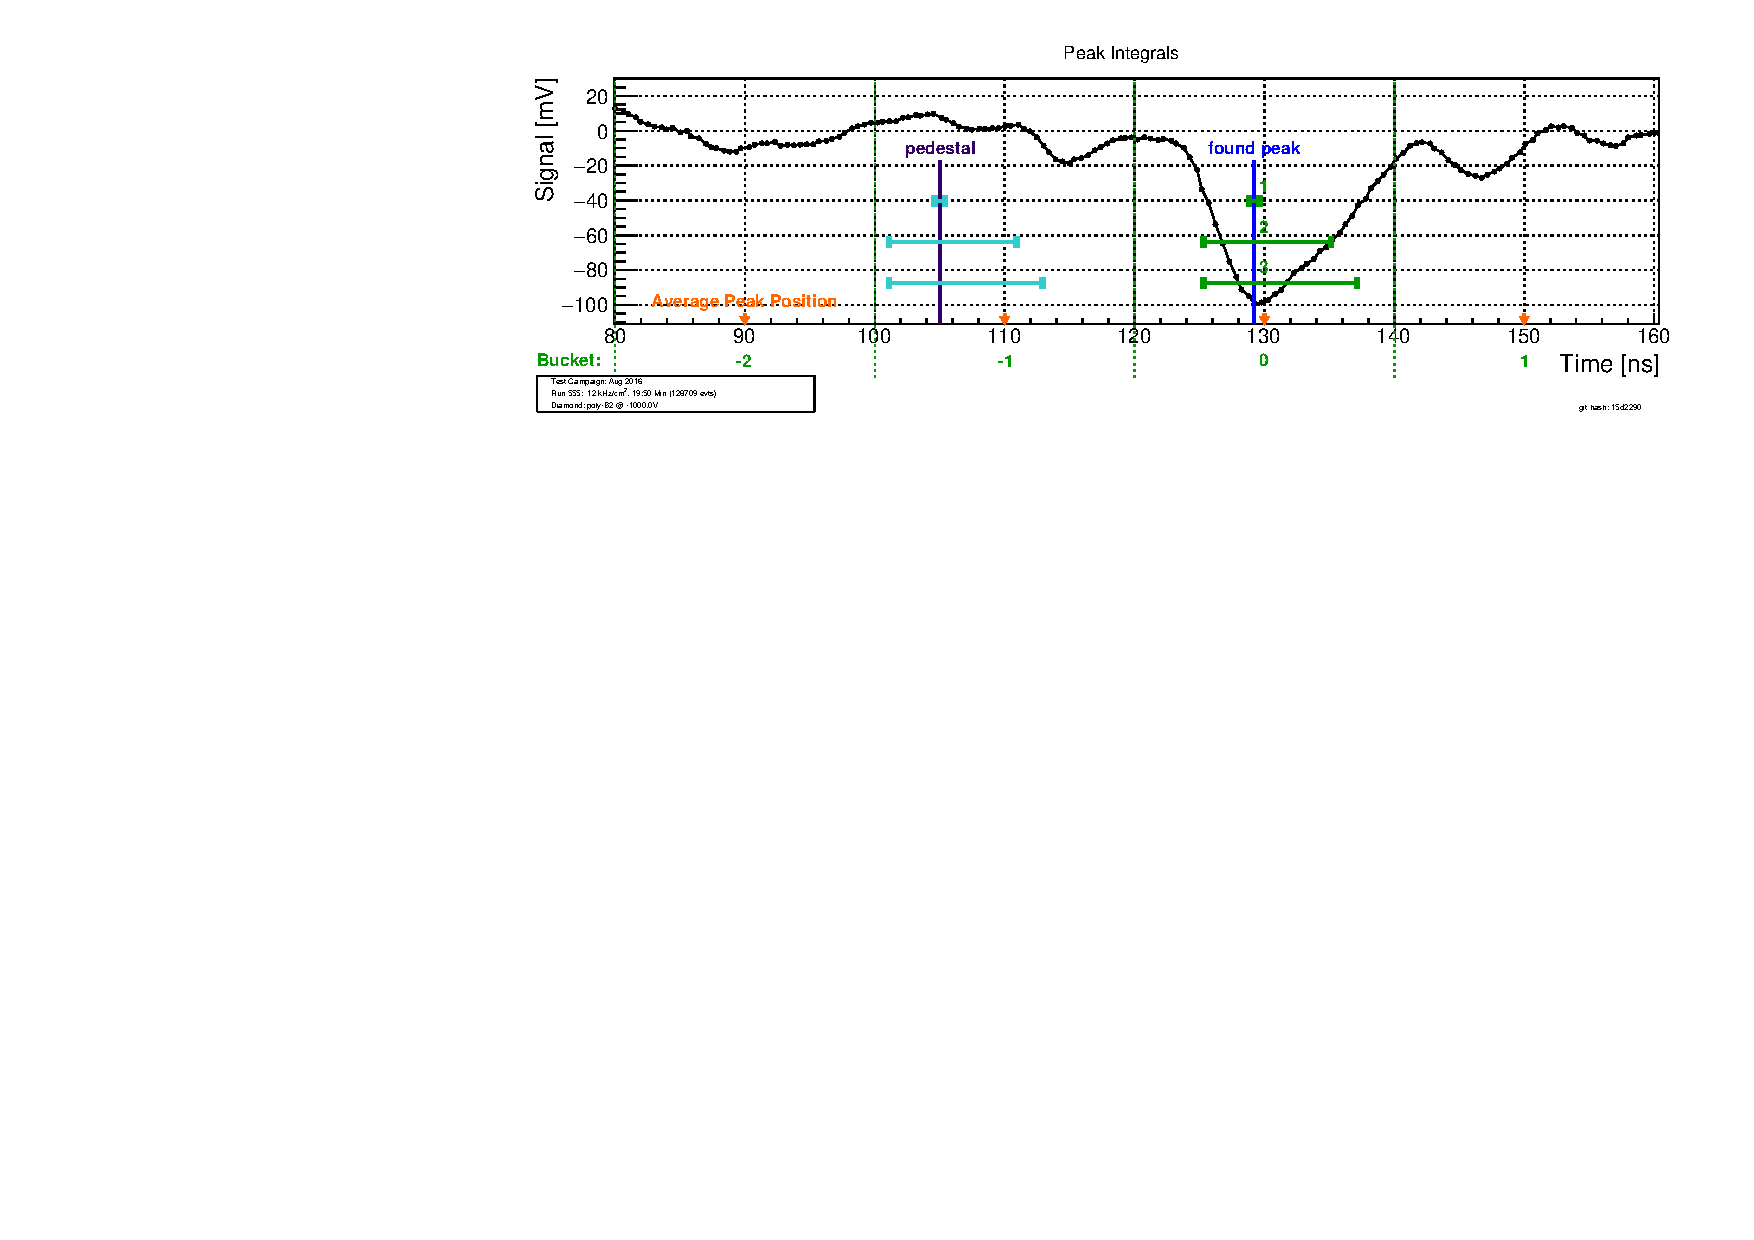
\includegraphics[angle=270, width=.8\textwidth]{IntegralPeaks}\\
	\end{center}
	\begin{itemize}
		\setlength{\itemsep}{\fill}
		\item finding the peak in the signal region (bucket 0)
		\item integrating the signal in given intervals around the found peak
		\item integrating the pedestal (base line $\rightarrow$ noise)
		\begin{itemize}
			\item using same intervals as for the signal in fixed position in bucket -1 (signals forbidden!)
		\end{itemize}
		\item optimizing the final interval by highest SNR (Integral / Pedestal Sigma)
		\item subtracting the pedestal from the signal integral on event-wise basis 
	\end{itemize}
\end{frame}
% new frame =======================
\begin{frame}
	\frametitle{Timing Correction}
	\begin{itemize}
		\item ring buffer cells of the digitizer have different sizes (\SI[separate-uncertainty = true]{\approx.5\pm.15}{ns})
		\item effective timing depends on starting cell of the buffer (=trigger cell)
		\item use trigger cell and measured cell length to get precise timing
	\end{itemize}
	\begin{minipage}{5.0cm}
		\centering
		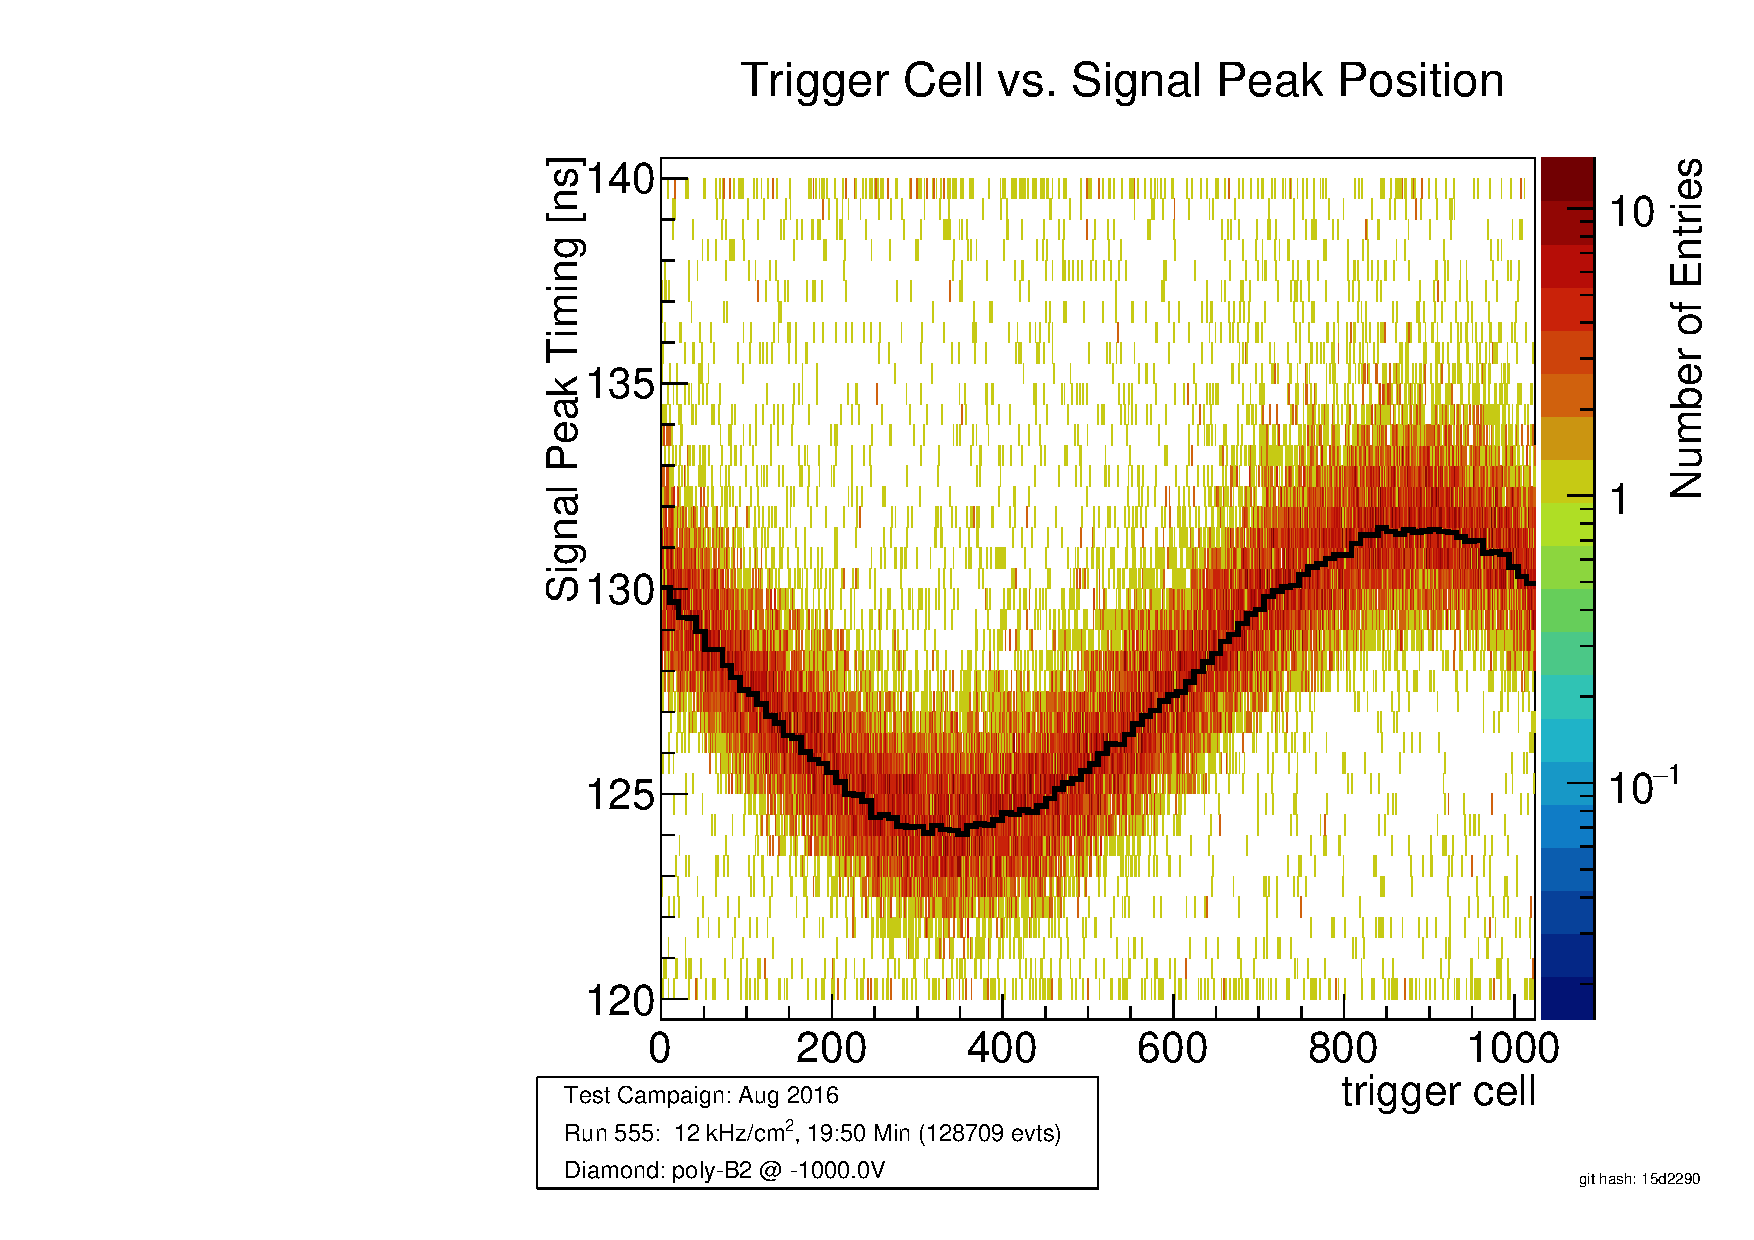
\includegraphics[angle=270, width=5cm]{TCVSPP}
	\end{minipage}
	\begin{minipage}{1.5cm}
		\centering
		Timing Correction\\
		$\longrightarrow$
	\end{minipage}
	\begin{minipage}{5.0cm}
		\centering
		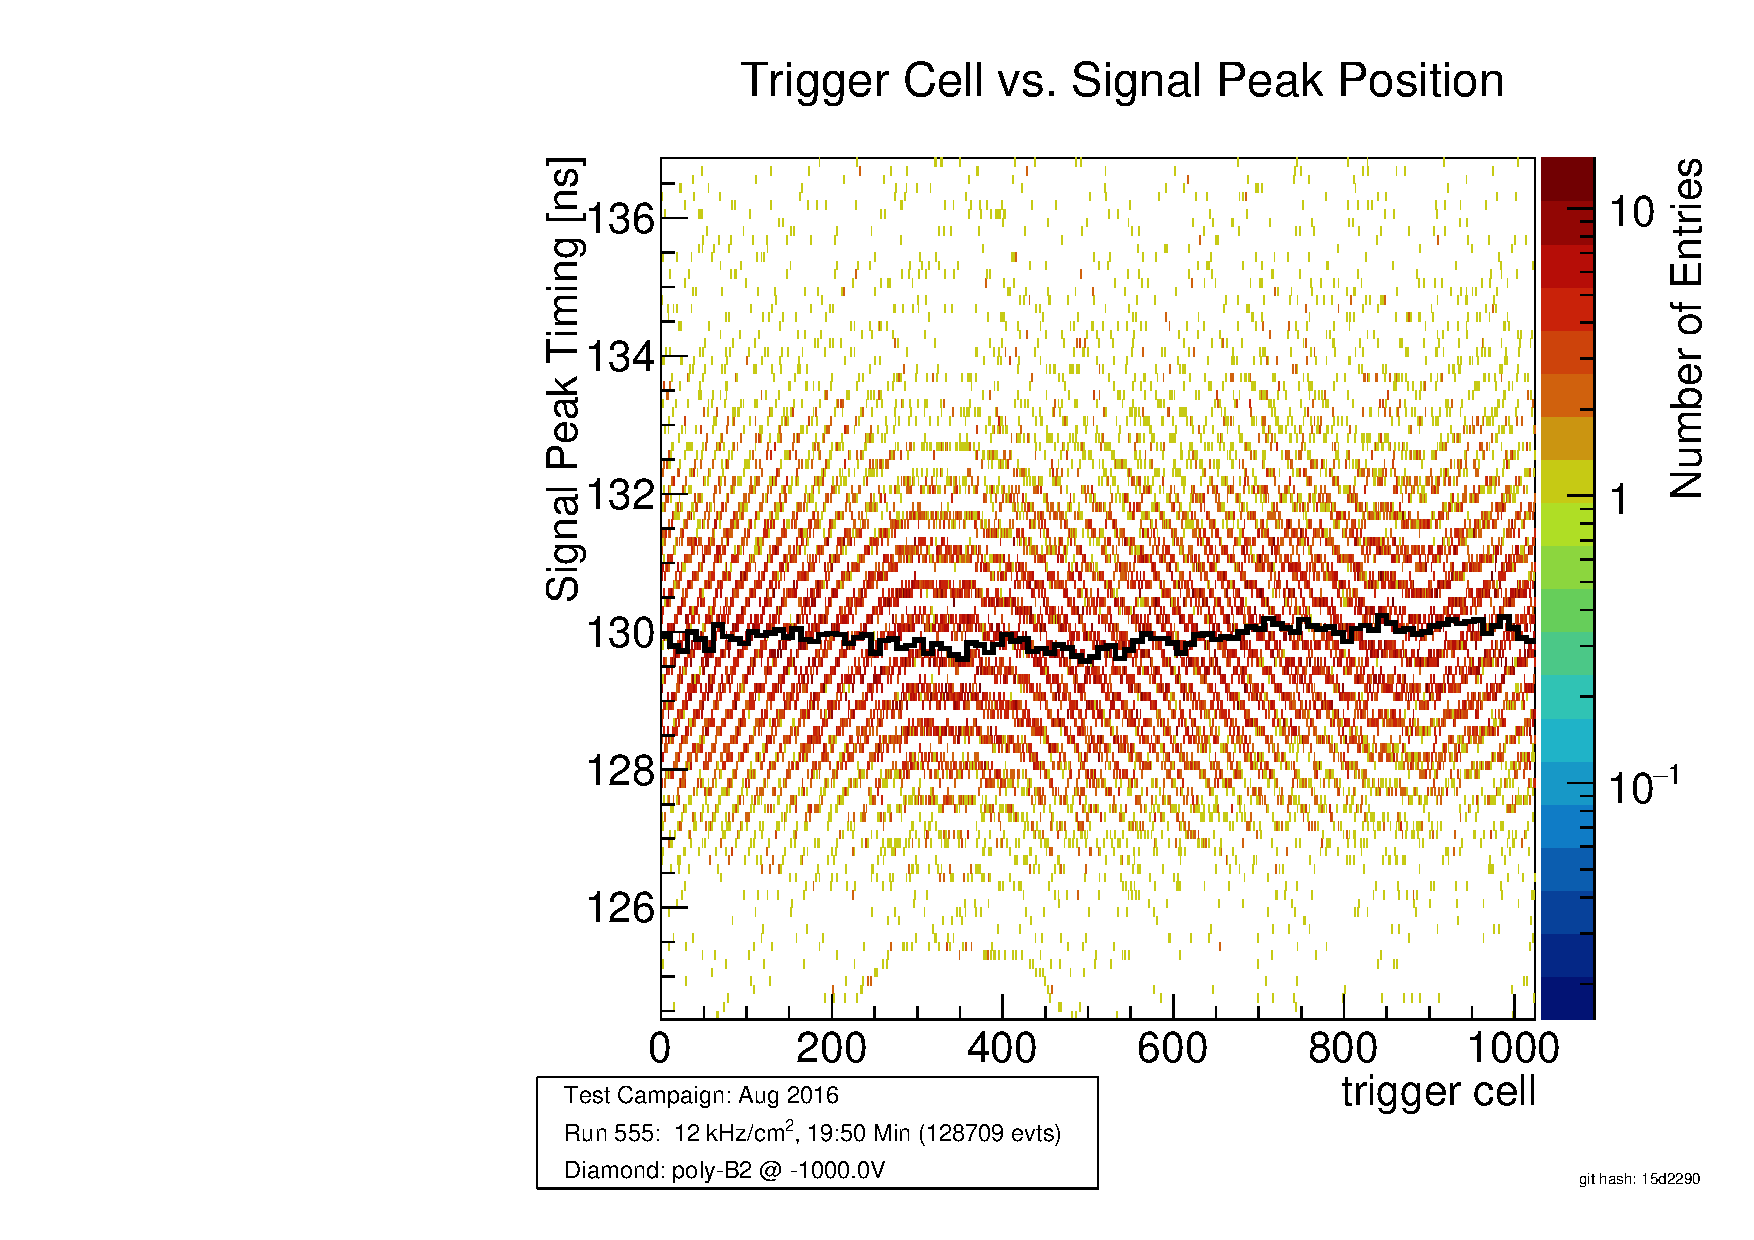
\includegraphics[angle=270, width=5cm]{TCVSPPCorr}
	\end{minipage}
\end{frame}
% new frame =======================
\begin{frame}
	\frametitle{Corrected Timing of the Signal Peaks}
	\vspace*{-20pt}
	\begin{center}
		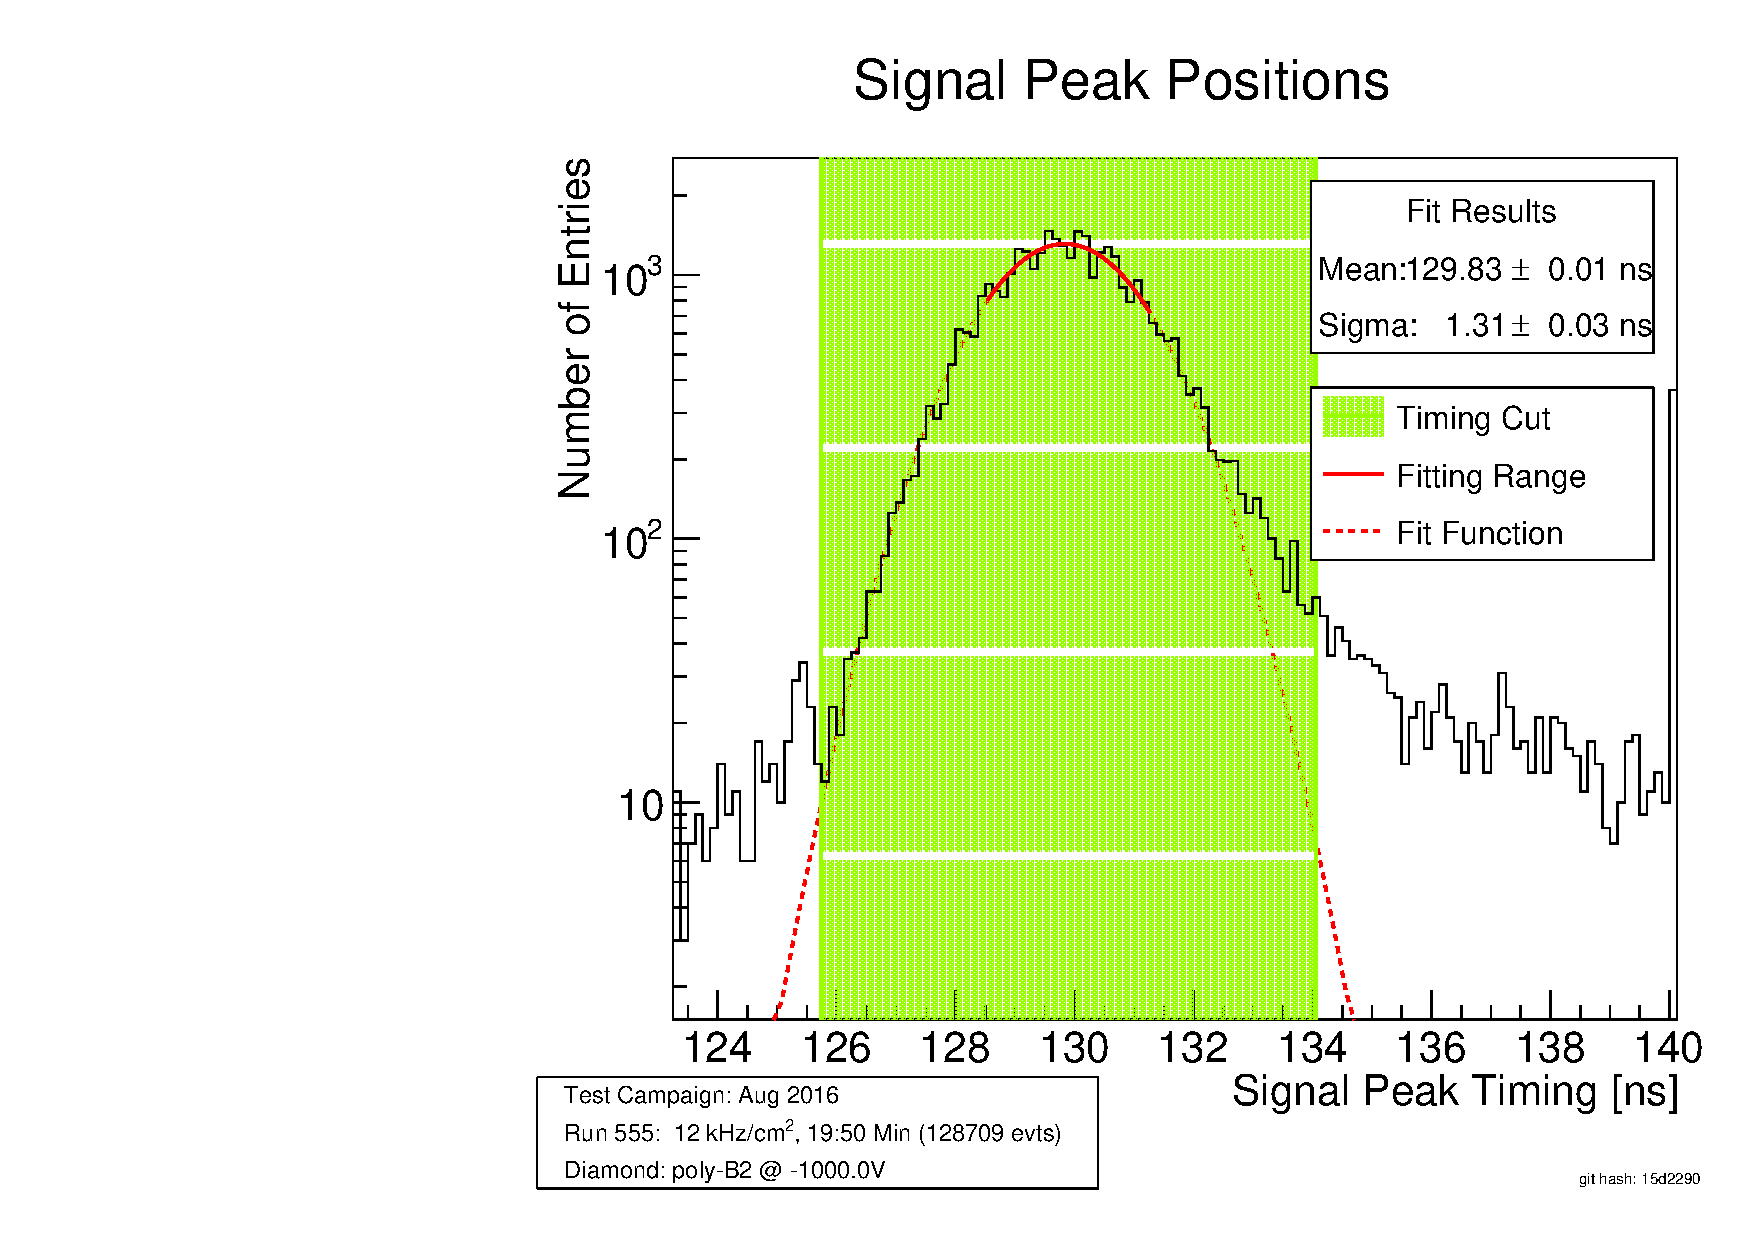
\includegraphics[angle=270, width=6cm]{SigPeakPos}\\
	\end{center}
	\begin{itemize}
		\item timing follows Gaussian distribution with $\upsigma=$ \SI[separate-uncertainty = true]{1.31\pm.03}{ns}
		\item use cut (\SI{4}{\upsigma}) based on this distribution to discard events with wrong timing 
		\begin{itemize}
			\item overlay of different buckets
		\end{itemize}
	\end{itemize}
\end{frame}
% ============================
\subsection{Event Cuts}
\begin{frame}
	\frametitle{Event Cuts}
	\begin{minipage}[c][.8\textheight]{7cm}
		\underline{\textbf{Exclude events:}}\s
		\begin{itemize}
			\small
			\setlength{\itemsep}{\fill}
			\item saturated: with saturated waveforms
			\item pulser: reference events 
			\item tracks: with incomplete tracks
			\item timing
			\item fiducial: track not in selected area of the diamond
		\end{itemize}
		\vspace*{1cm}
		\underline{\textbf{Also cuts on:}}\s
		\begin{itemize}
			\item $\upchi^{2}$ in $x$ and $y$, track angle, event range, pedestal sigma
		\end{itemize}
	\end{minipage}
	\hspace*{2pt}
	\begin{minipage}{4cm}
		\centering
		S129\\
		\vspace*{-5pt}
		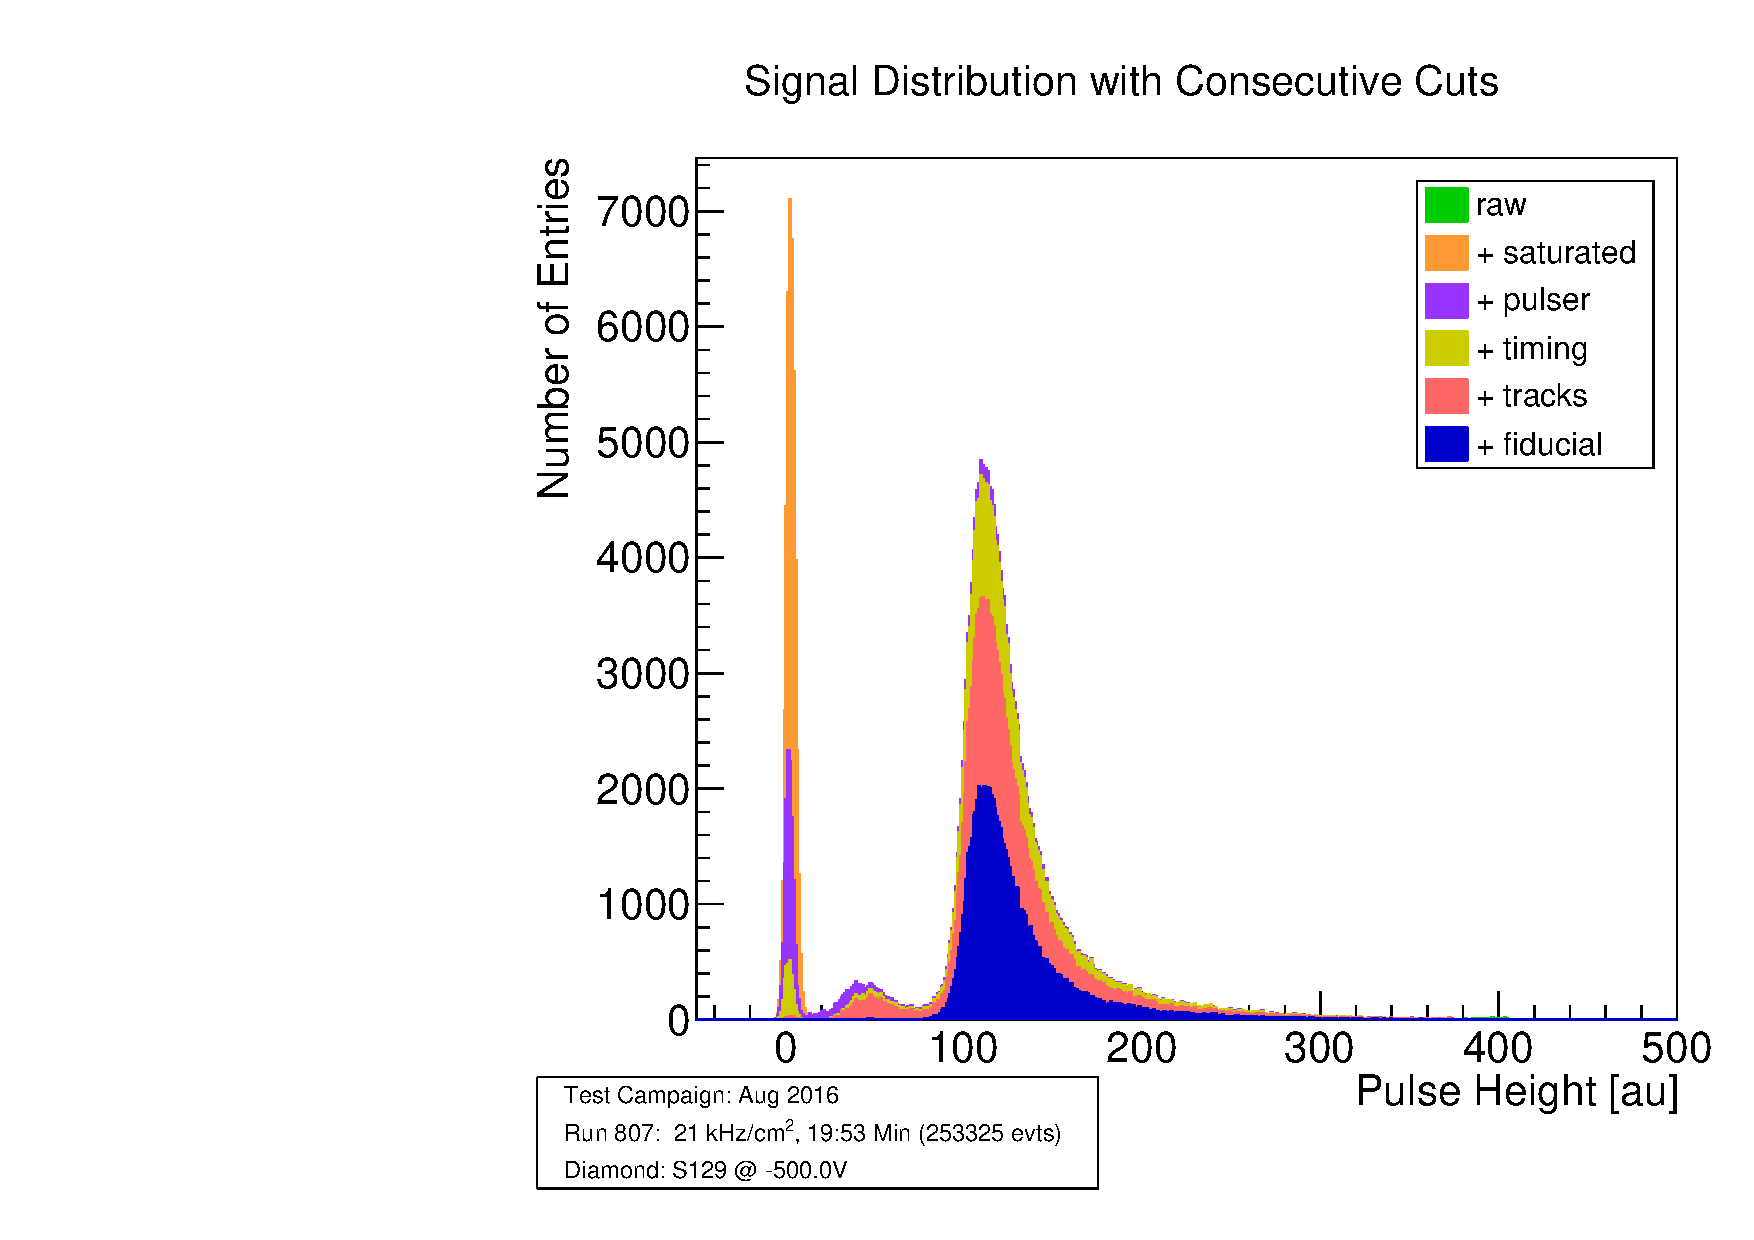
\includegraphics[angle=270, width=3.4cm]{Consecutive807}\\
		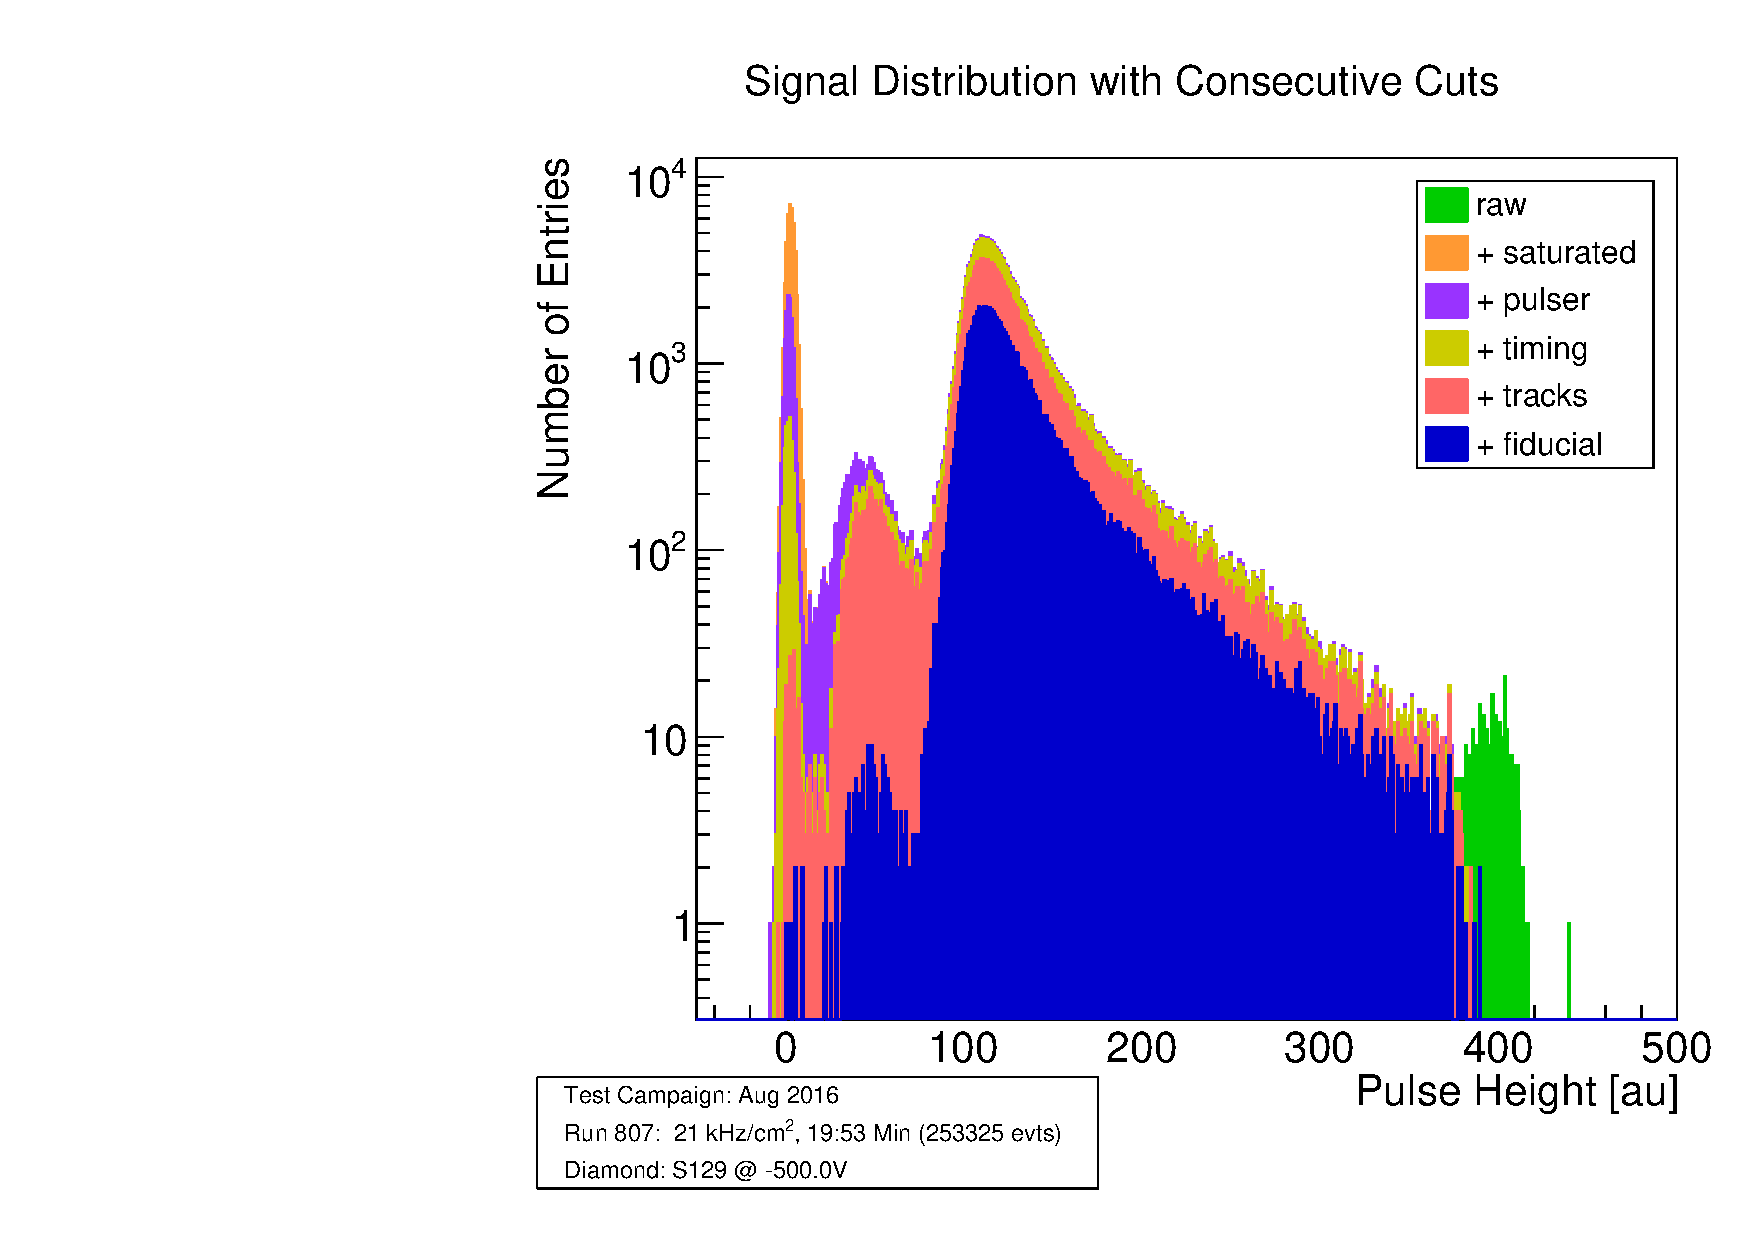
\includegraphics[angle=270, width=3.4cm]{ConsecutiveLog807}
	\end{minipage}
\end{frame}
% new frame =======================
\begin{frame}
	\frametitle{Pulse Height Distribution}
	\begin{minipage}{4cm}
		\centering 
		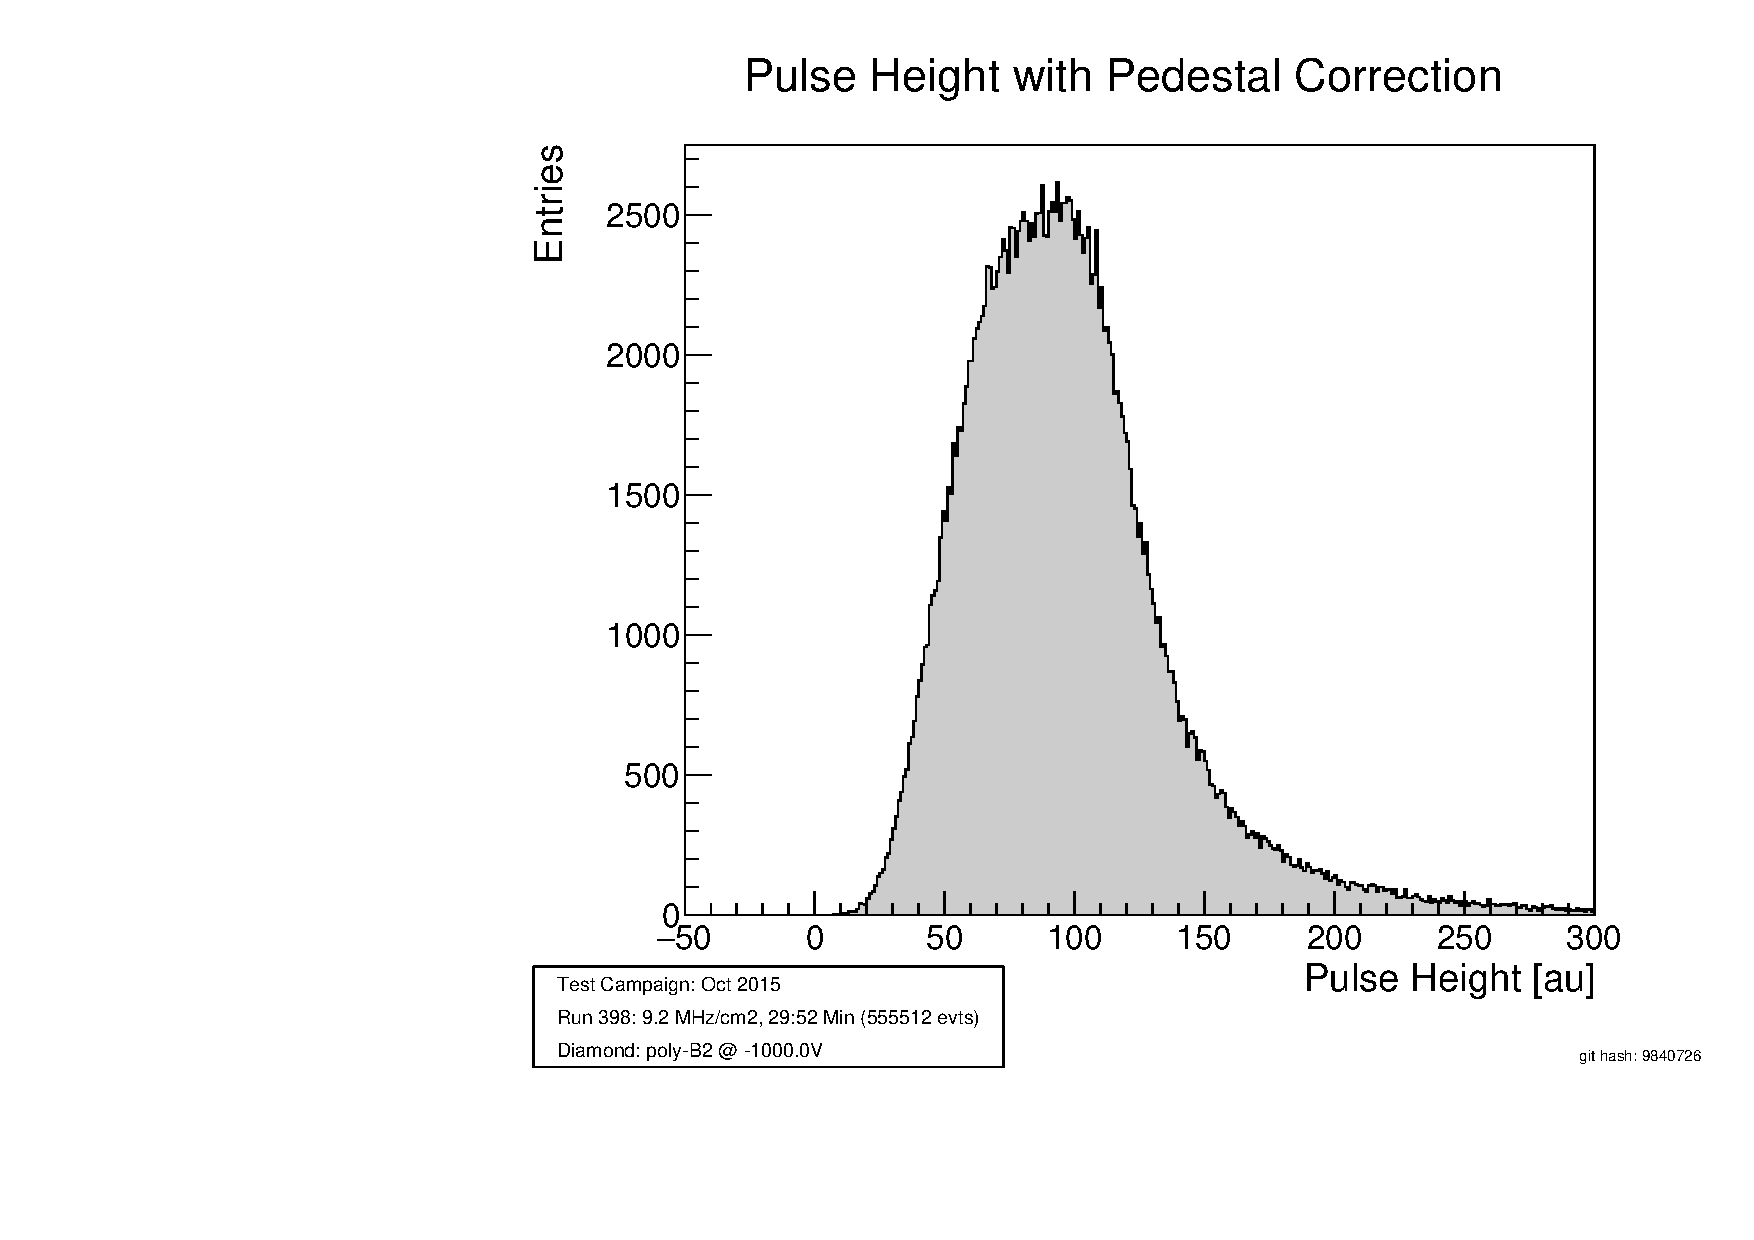
\includegraphics[angle=270, width=3.0cm]{Landau}
	\end{minipage}
	\hspace*{2pt}
	\begin{minipage}{6.5cm}
		\centering
		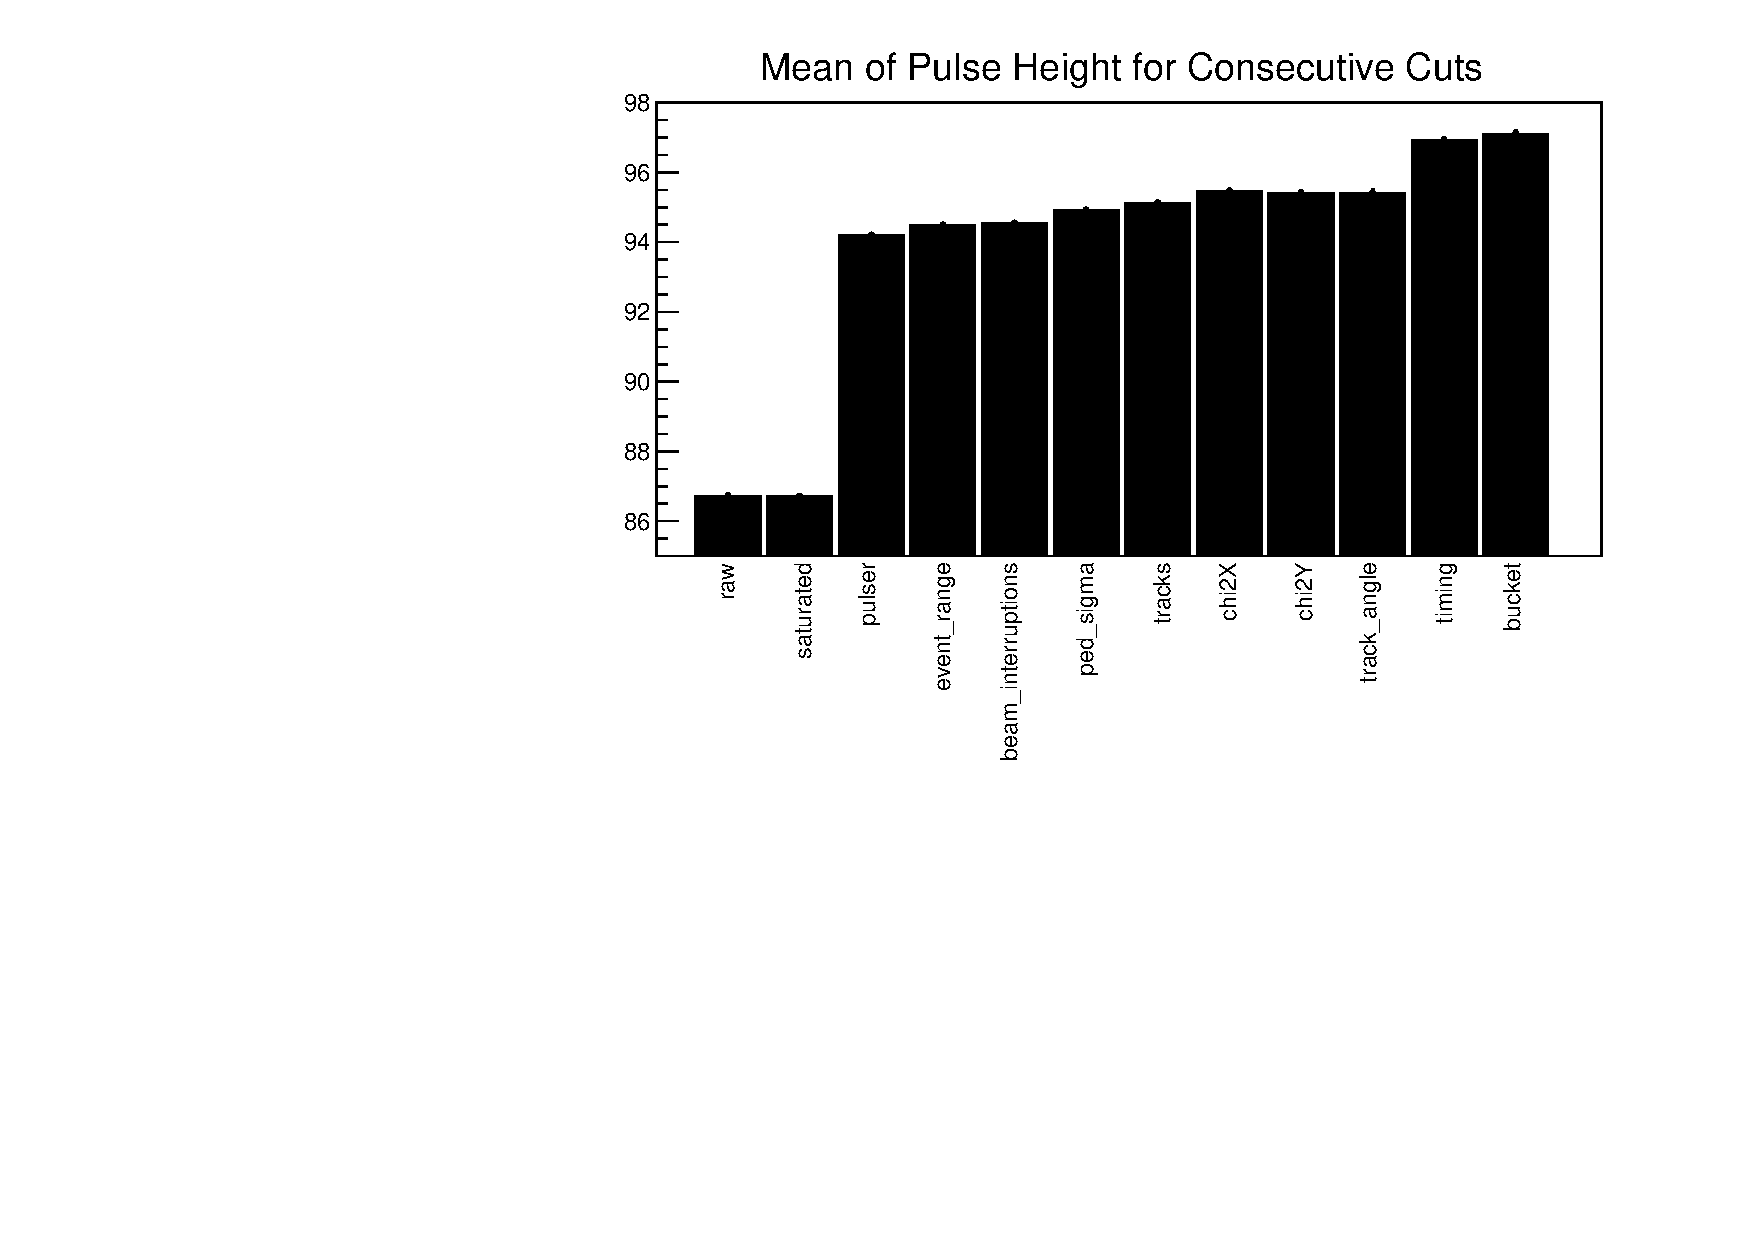
\includegraphics[angle=270, width=3.0cm]{CutMeans}
	\end{minipage}
	\begin{minipage}{6cm}
		\begin{itemize}
			\item pedestal almost completely gone after application of the cuts 
			\item mean of the pulse height increases significantly due to cuts (pedestal goes away)
		\end{itemize}
	\end{minipage}
	\hspace*{2pt}
	\begin{minipage}{5cm}
		\centering
		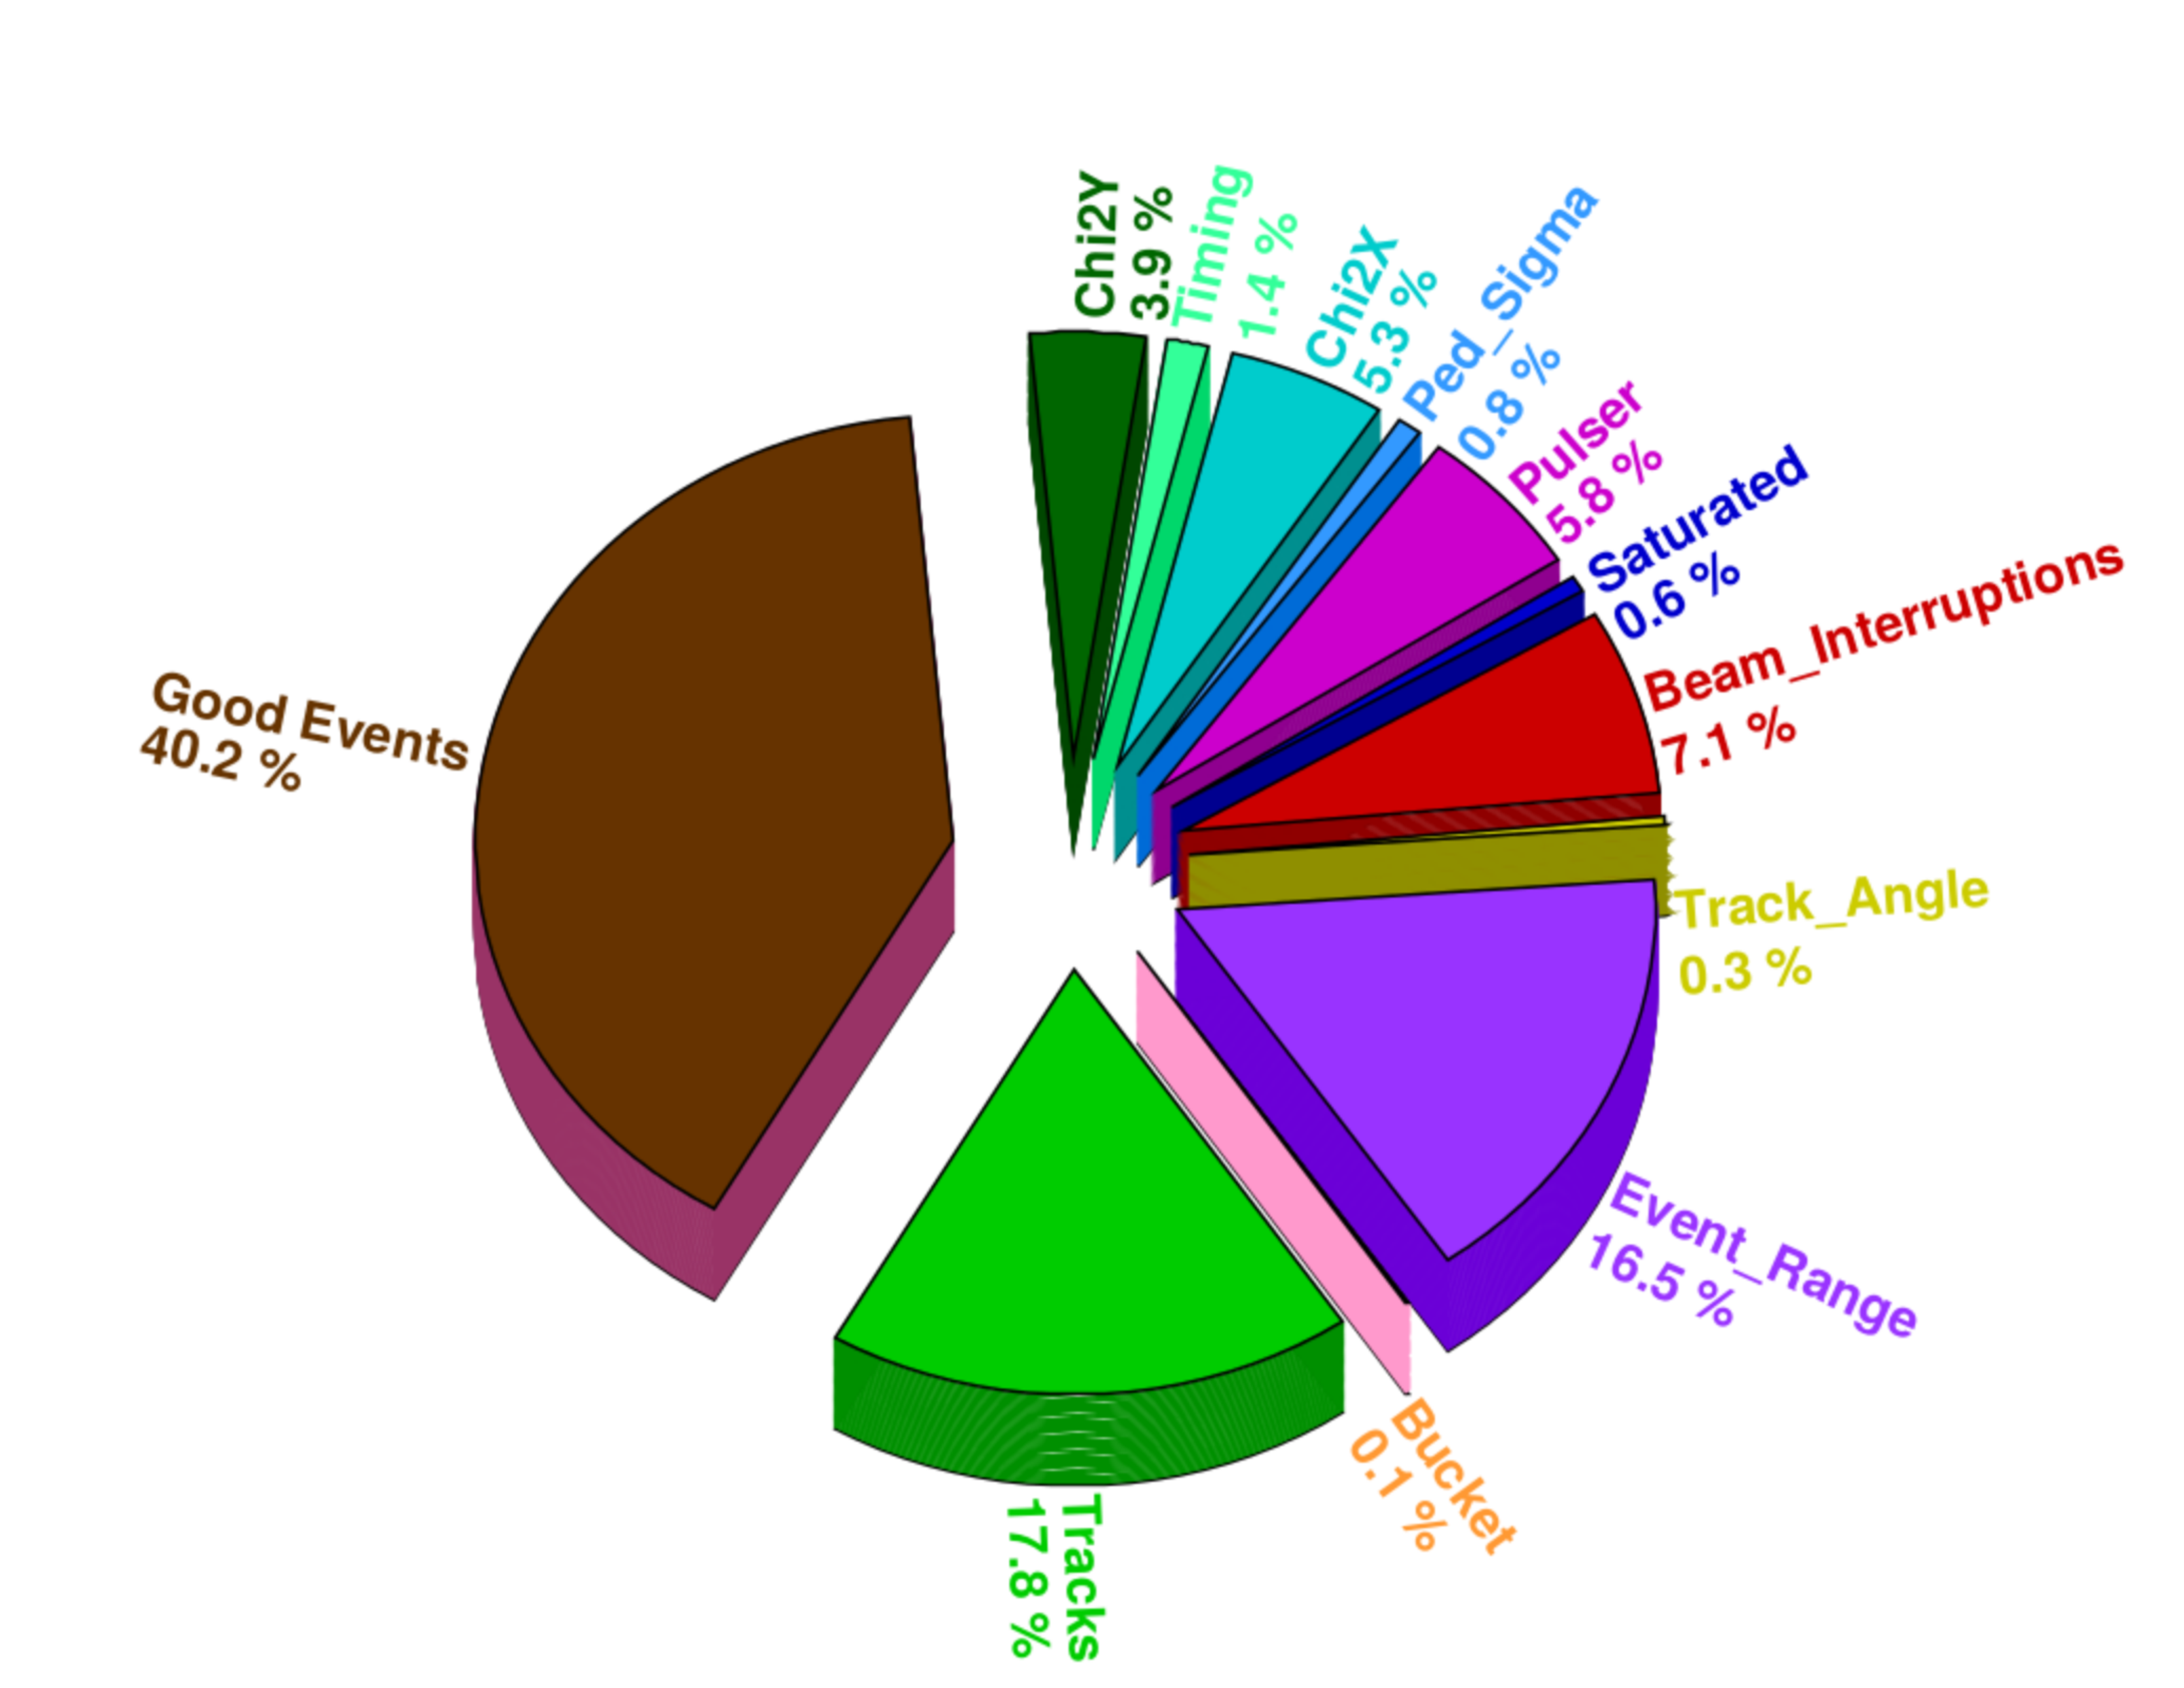
\includegraphics[angle=270, width=4cm]{Cuts}
	\end{minipage}
\end{frame}
% % ============================
% \subsection{Signal Map}
% \begin{frame}
% 	\frametitle{Signal Map}
% 	\begin{center}
% 		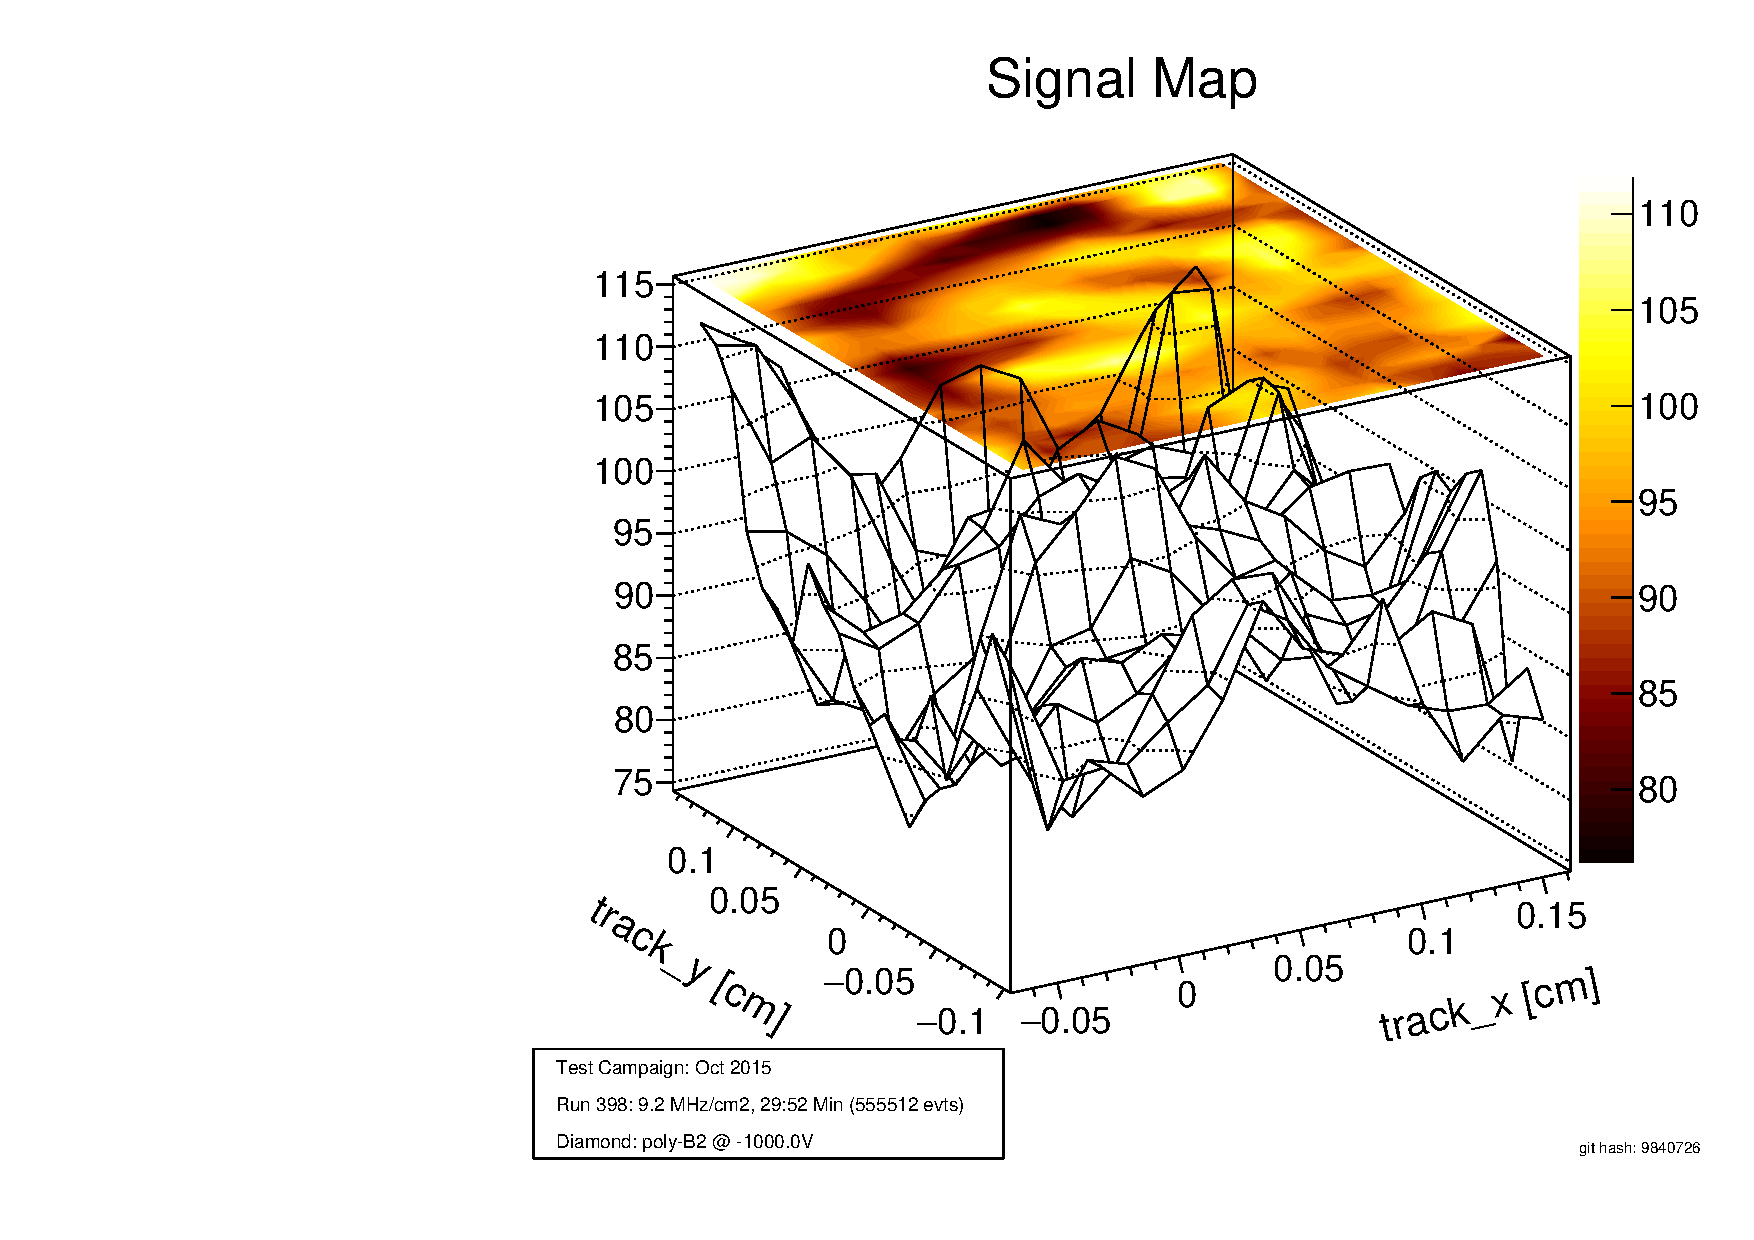
\includegraphics[angle=270, width=5.5cm]{SignalMap}\\
% 	\end{center}
% 	\begin{itemize}
% 		\item different regions inside the diamond yield different average pulse heights
% 		\item does not change with rate or time
% 	\end{itemize}
% \end{frame}
% END
% ====================================================================================
% BEGIN RESULTS
% ====================================================================================
\section{Preliminary Results}
% ============================
\subsection{S129 (elementsix - single crystal)}
\begin{frame}
	\frametitle{S129 @ $-$\SI{500}{V} - unirradiated}
	\def \sp {3.7cm}
	\begin{minipage}{\sp}
		\centering
		October 2015 
		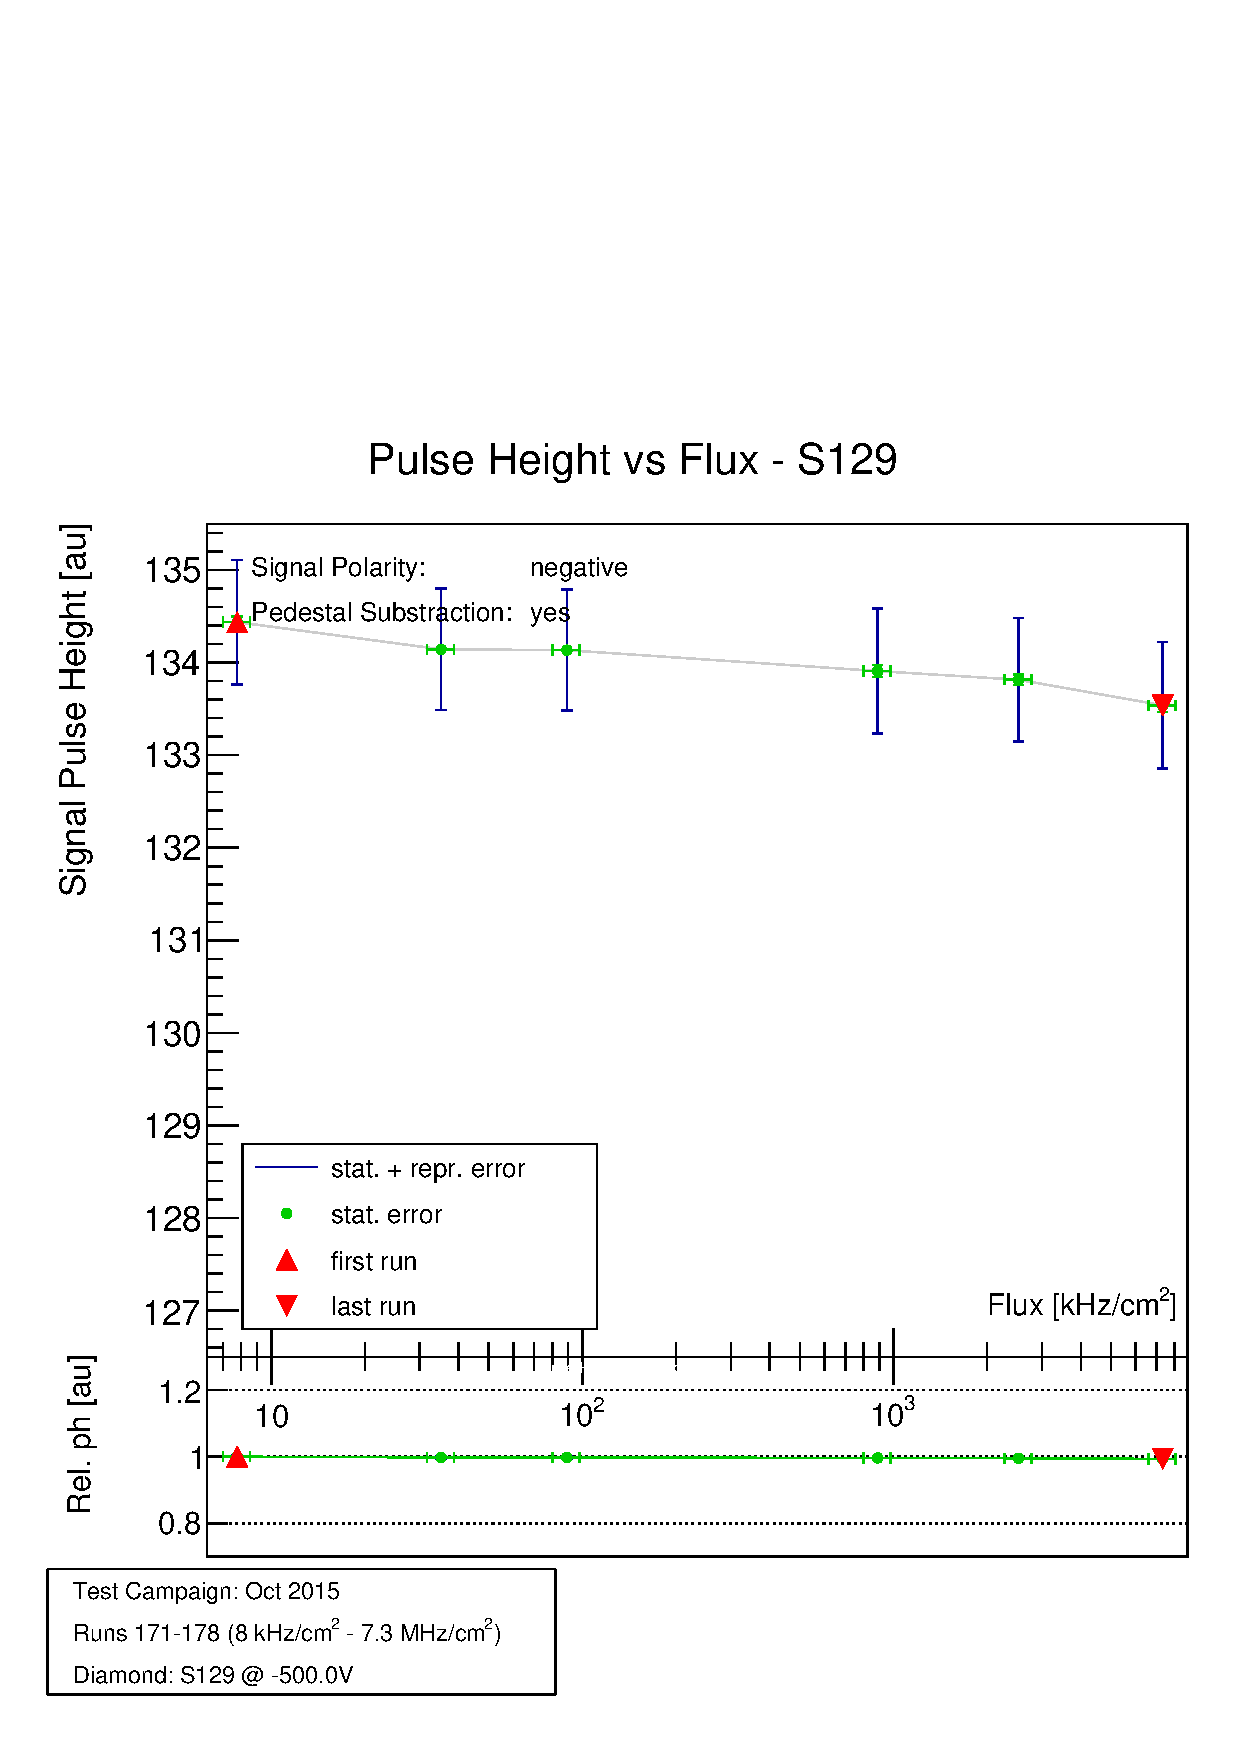
\includegraphics[width=\sp]{CPH1608_03}\\
		noise $\upsigma\approx$ \SI{2.6}{au}
	\end{minipage}
	\hspace*{2pt}
	\begin{minipage}{\sp}
		\centering
		August 2016 - begin
		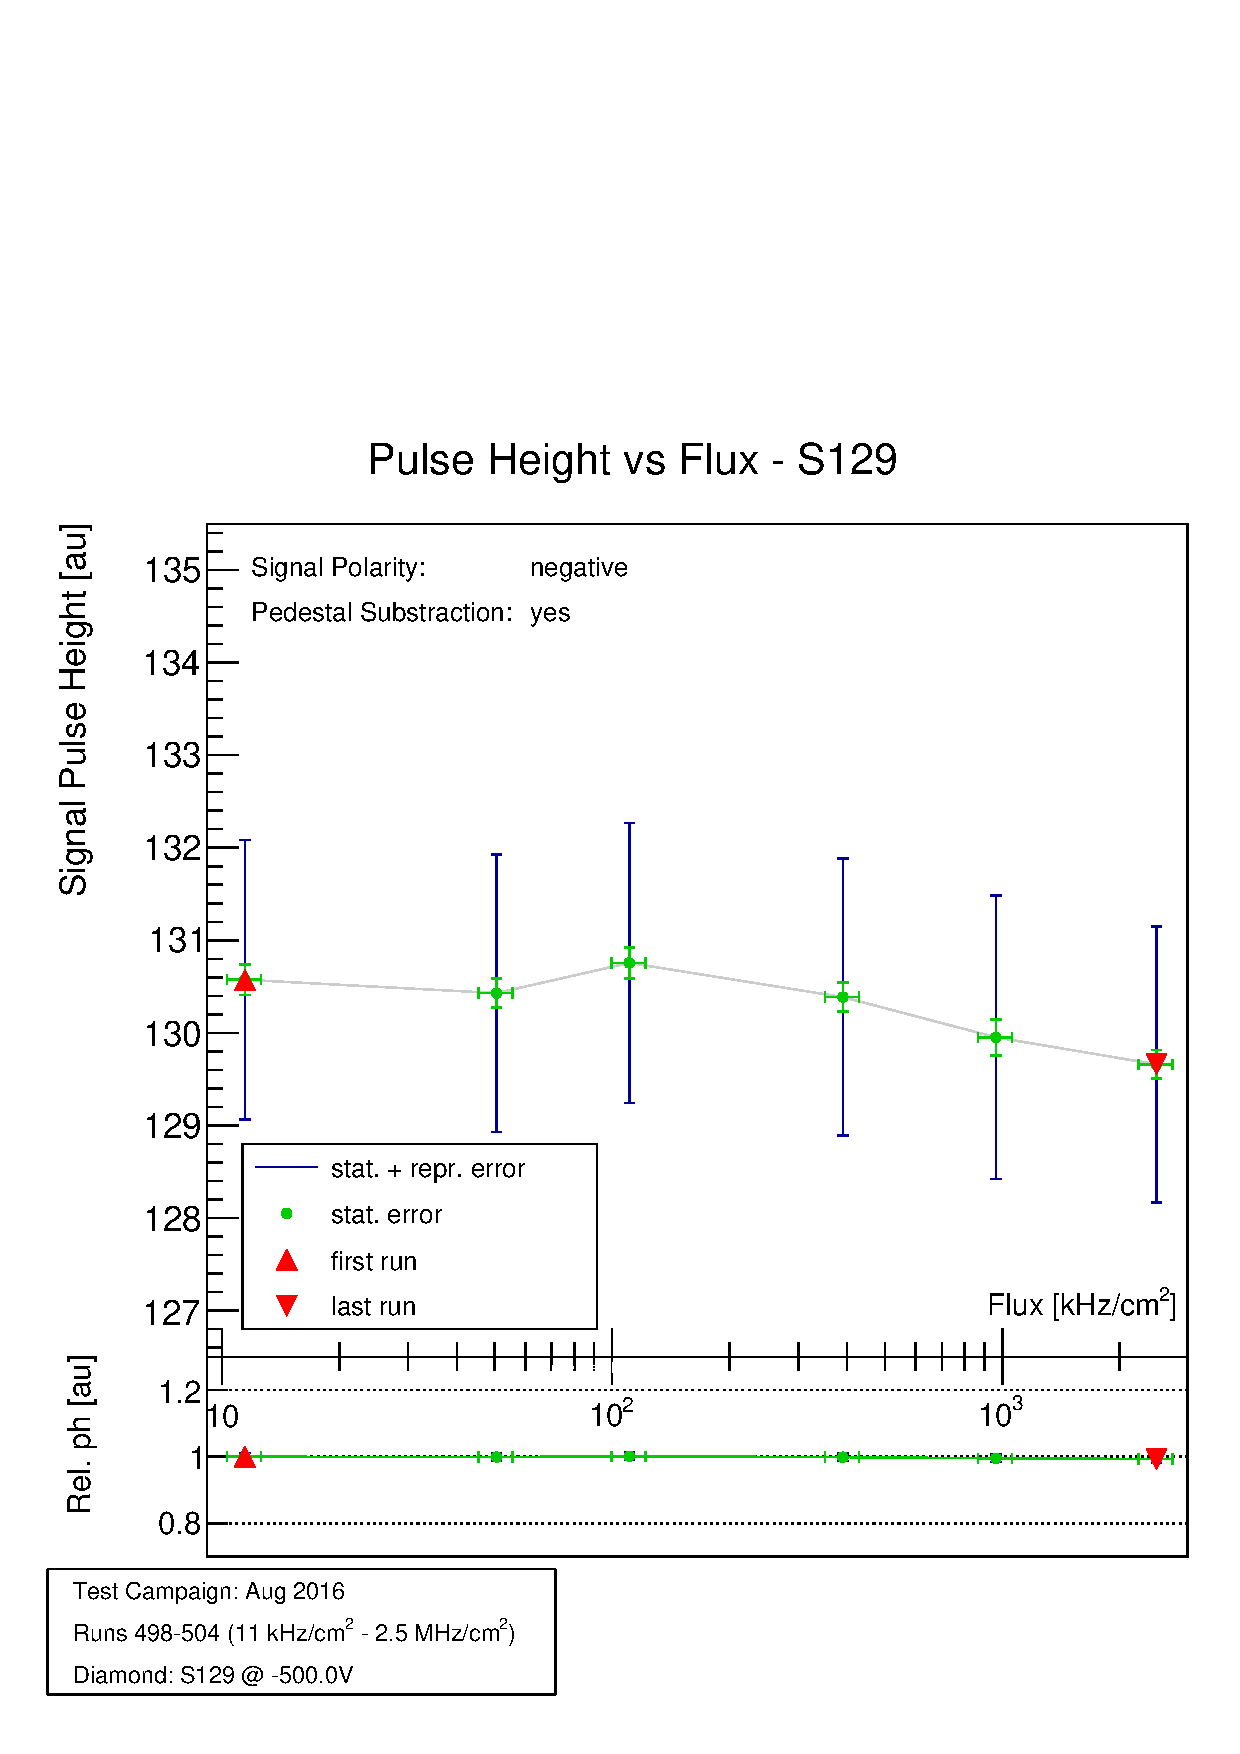
\includegraphics[width=\sp]{CPH1510_08_1}\\
		noise $\upsigma\approx$ \SI{2.6}{au}
	\end{minipage}
	\hspace*{2pt}
	\begin{minipage}{\sp}
		\centering
		August 2016 - end
		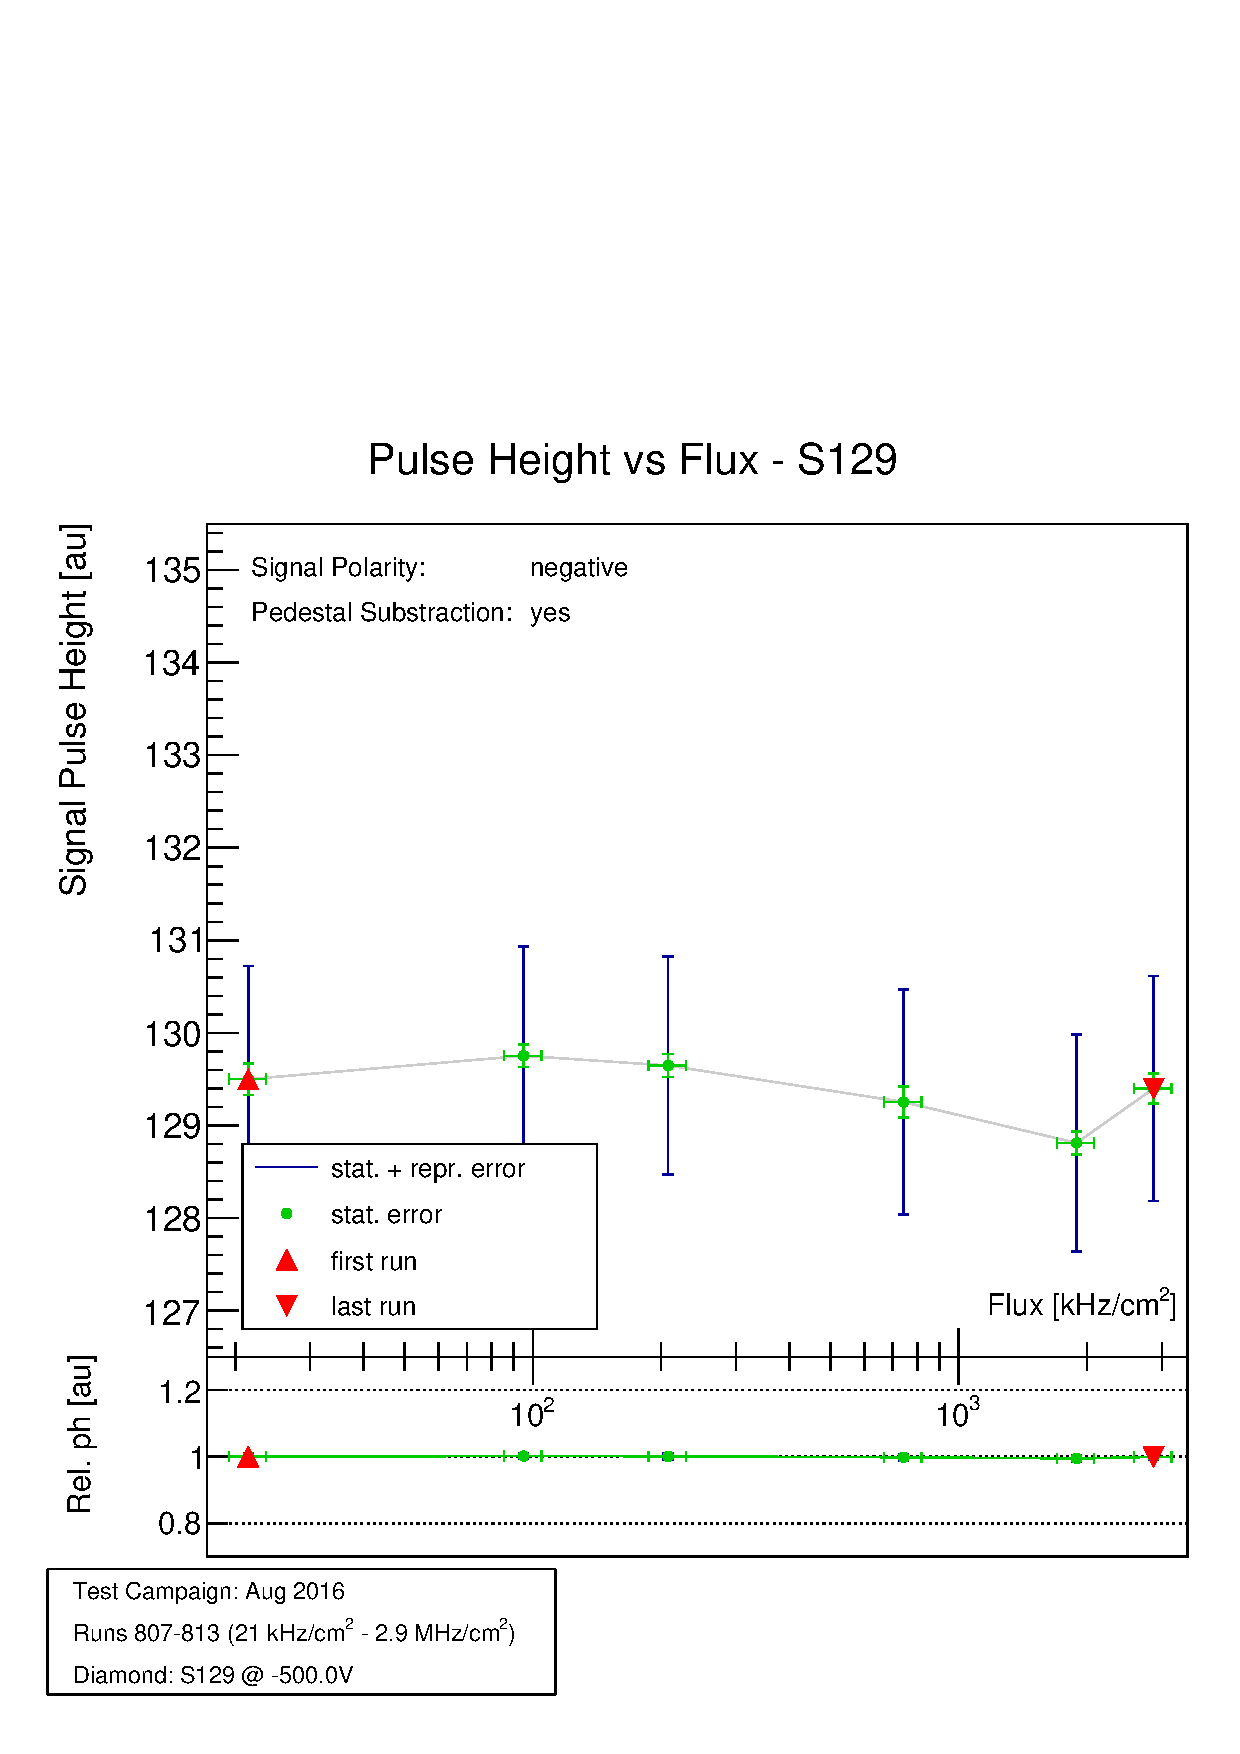
\includegraphics[width=\sp]{CPH1510_18_1}\\
		noise $\upsigma \approx$ \SI{2.6}{au}
	\end{minipage}\s
	\begin{itemize}
		\item measurements taken under the same conditions
		\item noise stays the same
		\item pulse height very stable
	\end{itemize}
\end{frame}
% ============================
\subsection{II6-B2 (II-VI - poly crystal)}
\begin{frame}
	\frametitle{II6-B2 @ $-$\SI{1000}{V}}
	\begin{minipage}{3.7cm}
		\centering
		August 2016 - \\unirradiated
		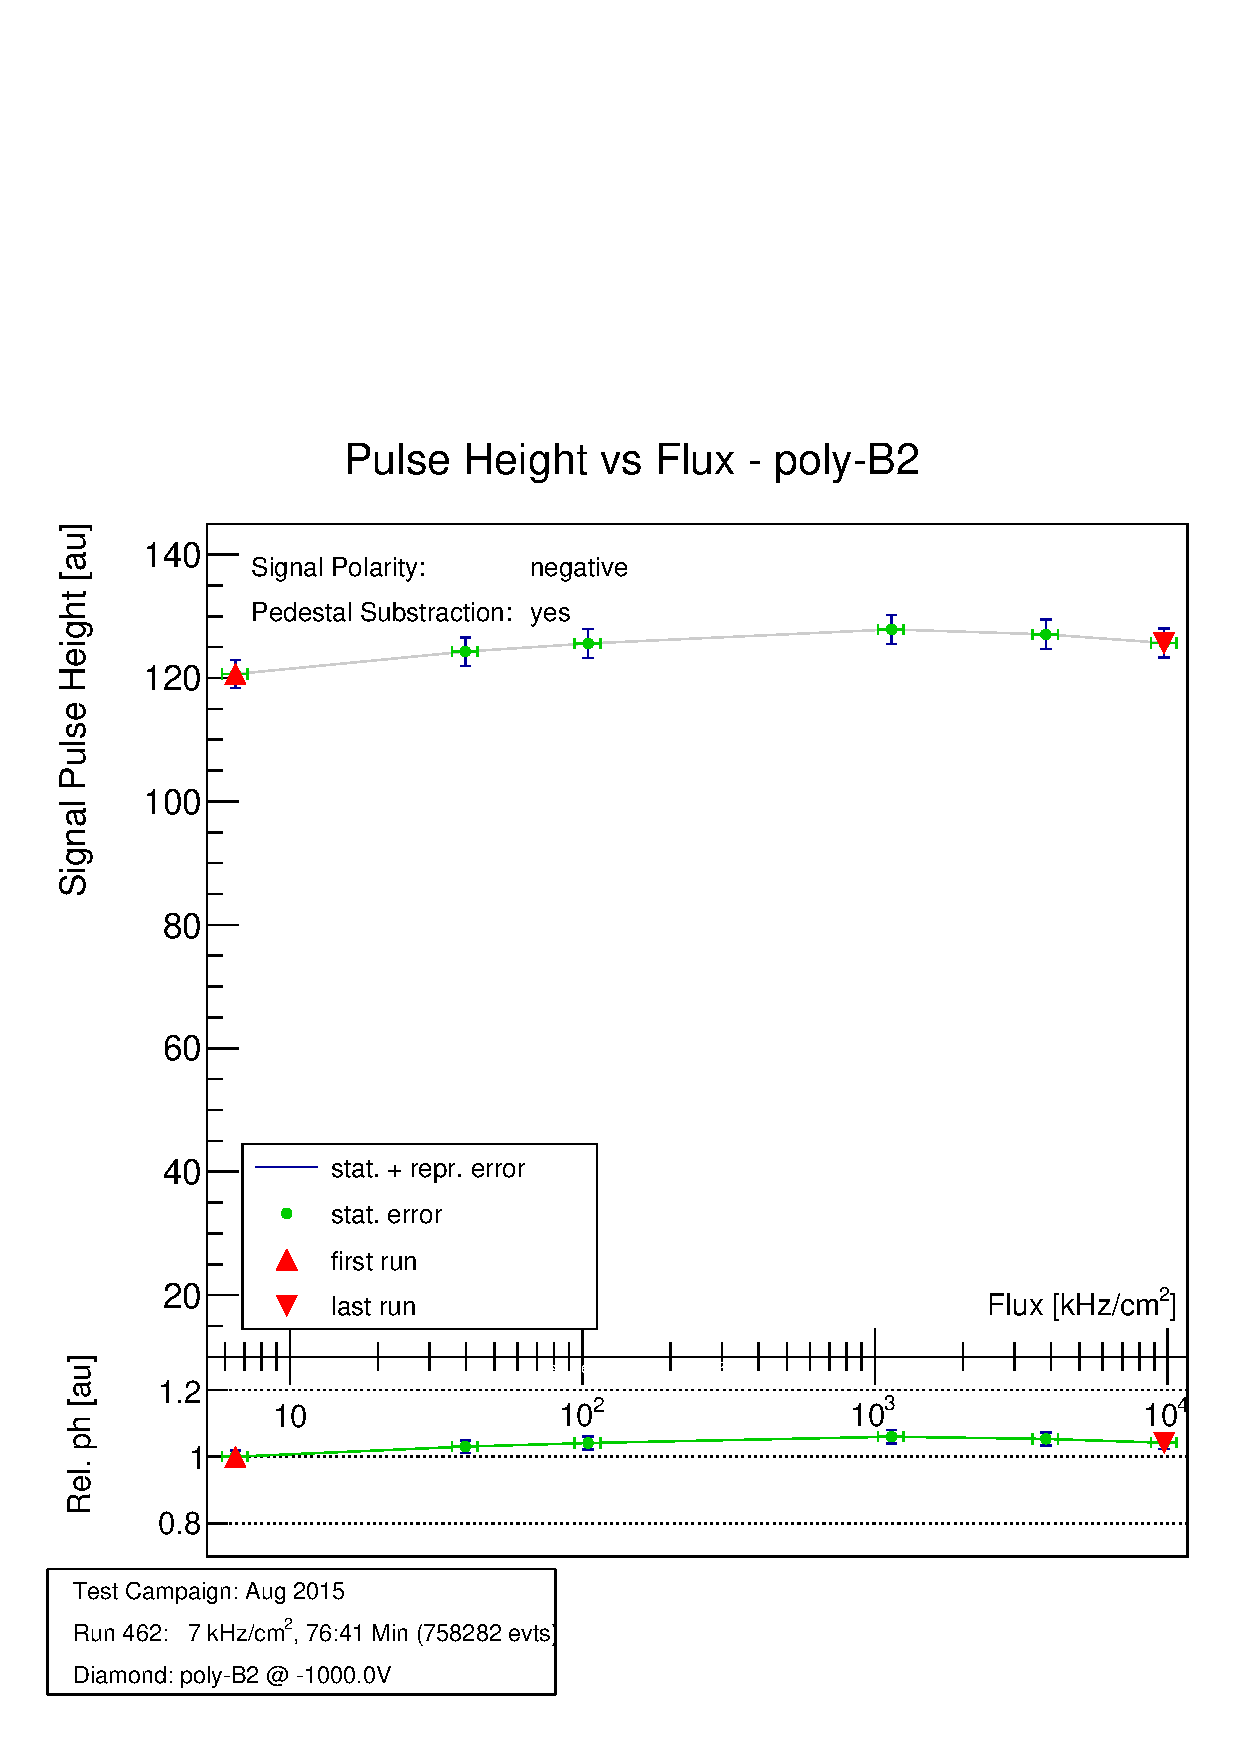
\includegraphics[width=3.7cm]{CPH1508_13_2.pdf}\\
		noise $\upsigma\approx$ \SI{4.9}{au}
	\end{minipage}
	\hspace*{2pt}
	\begin{minipage}{3.7cm}
		\centering
		October 2015 - \SI[exponent-product = \cdot]{5e14}{n/cm^{2}}
		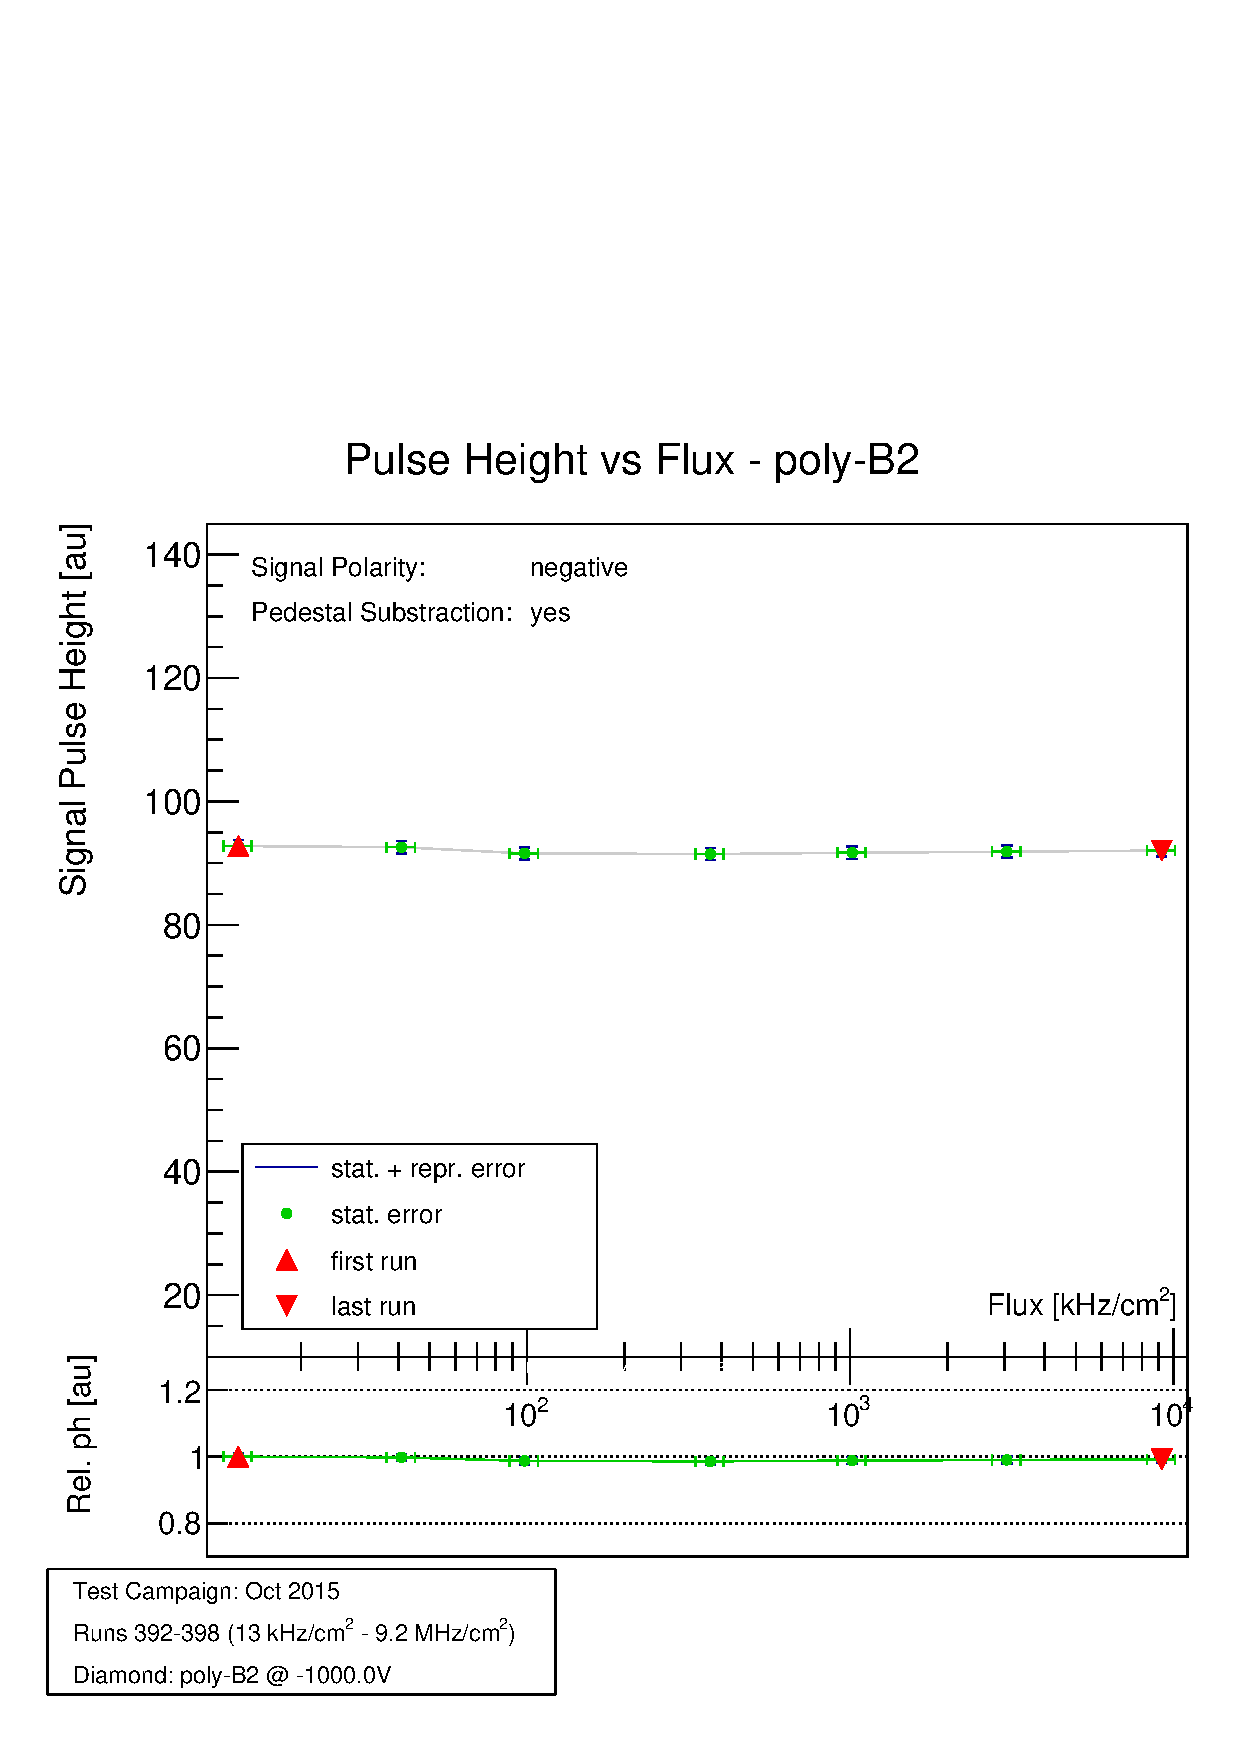
\includegraphics[width=3.7cm]{CPH1510_08_2.pdf}\\
		noise $\upsigma\approx$ \SI{4.9}{au}
	\end{minipage}
	\hspace*{2pt}
	\begin{minipage}{3.7cm}
		\centering
		August 2016 - \SI[exponent-product = \cdot]{1e15}{n/cm^{2}}
		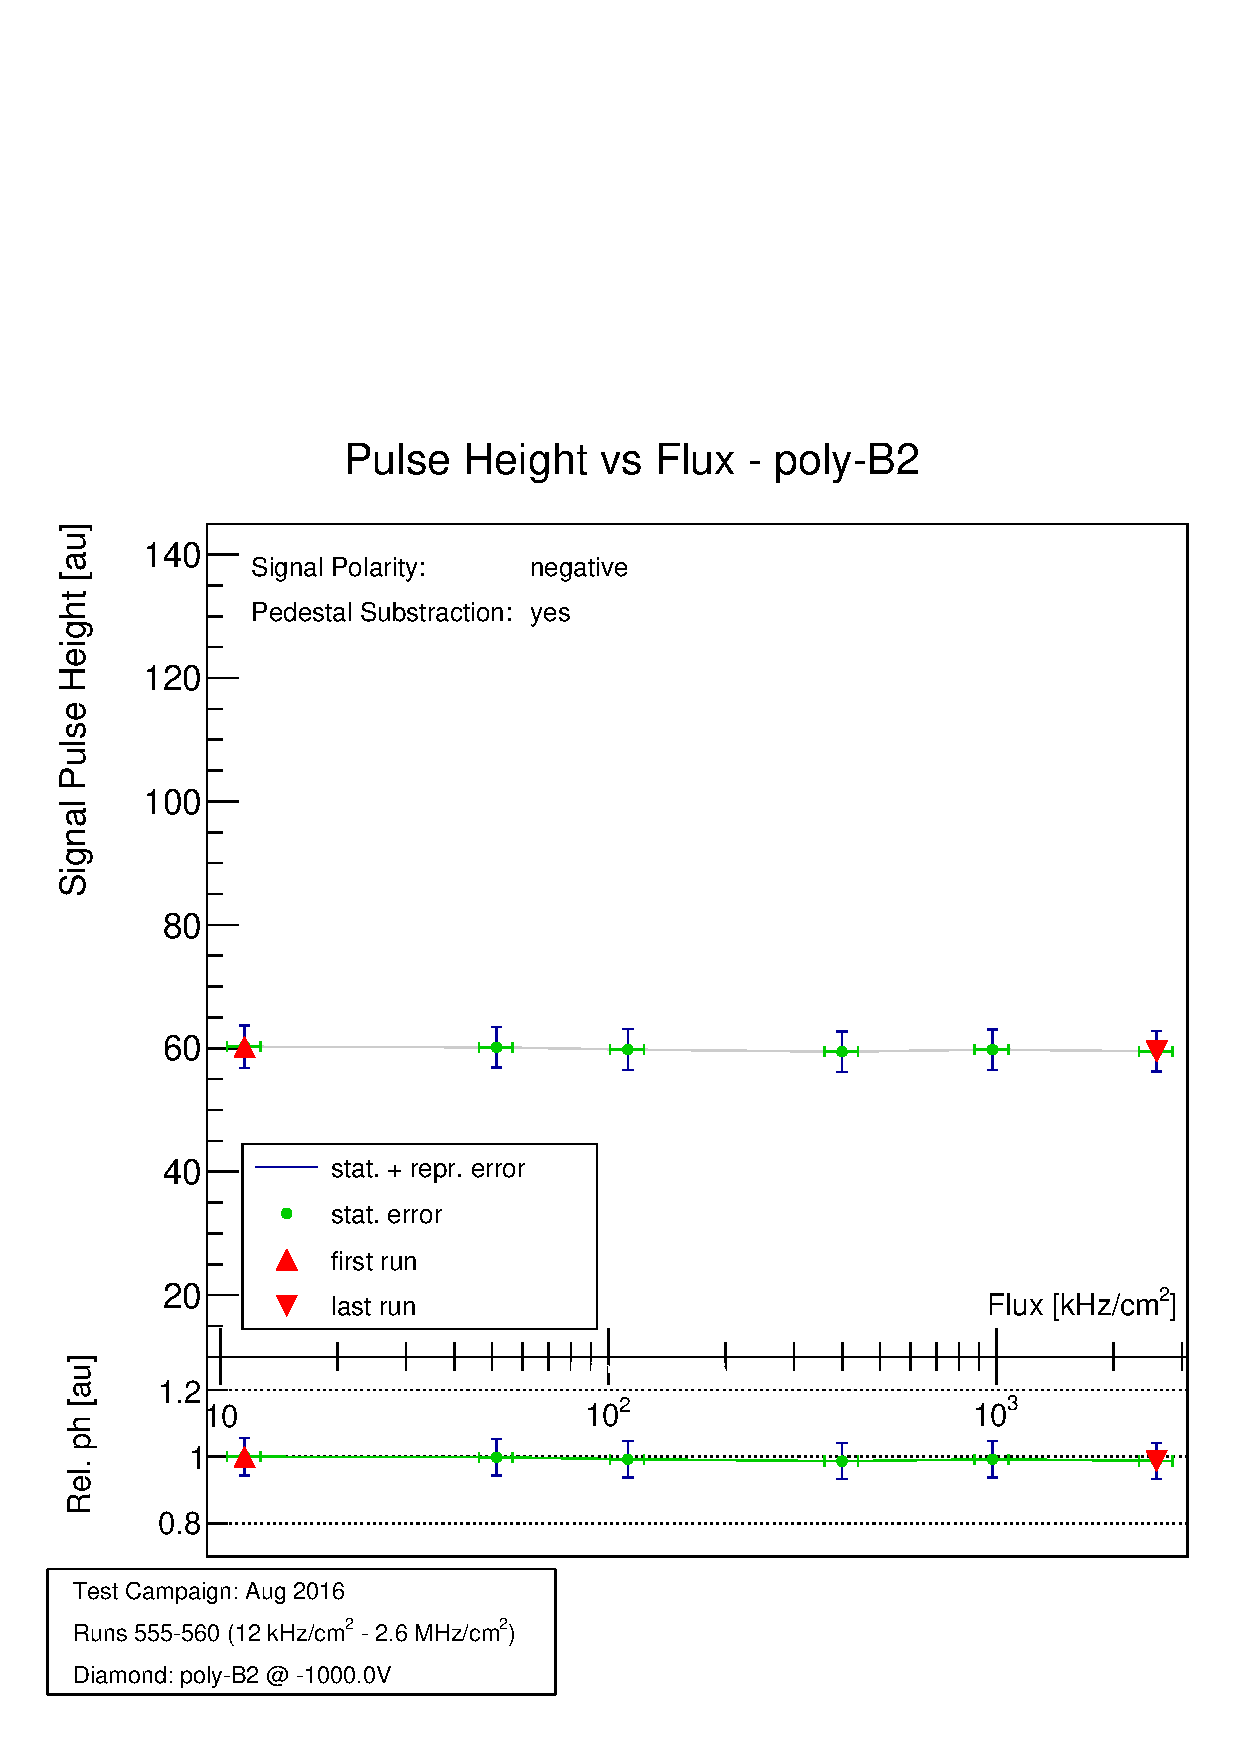
\includegraphics[width=3.7cm]{CPH1608_09_1_2.pdf}\\
		noise $\upsigma \approx$ \SI{4.9}{au}
	\end{minipage}\s
	\begin{itemize}
		\item pulse height very stable after irradiation
		\item noise stays the same
	\end{itemize}
\end{frame}
% new frame =======================
\begin{frame}
	\begin{minipage}{3.1cm}
		\centering
		August 2016 - \\unirradiated
		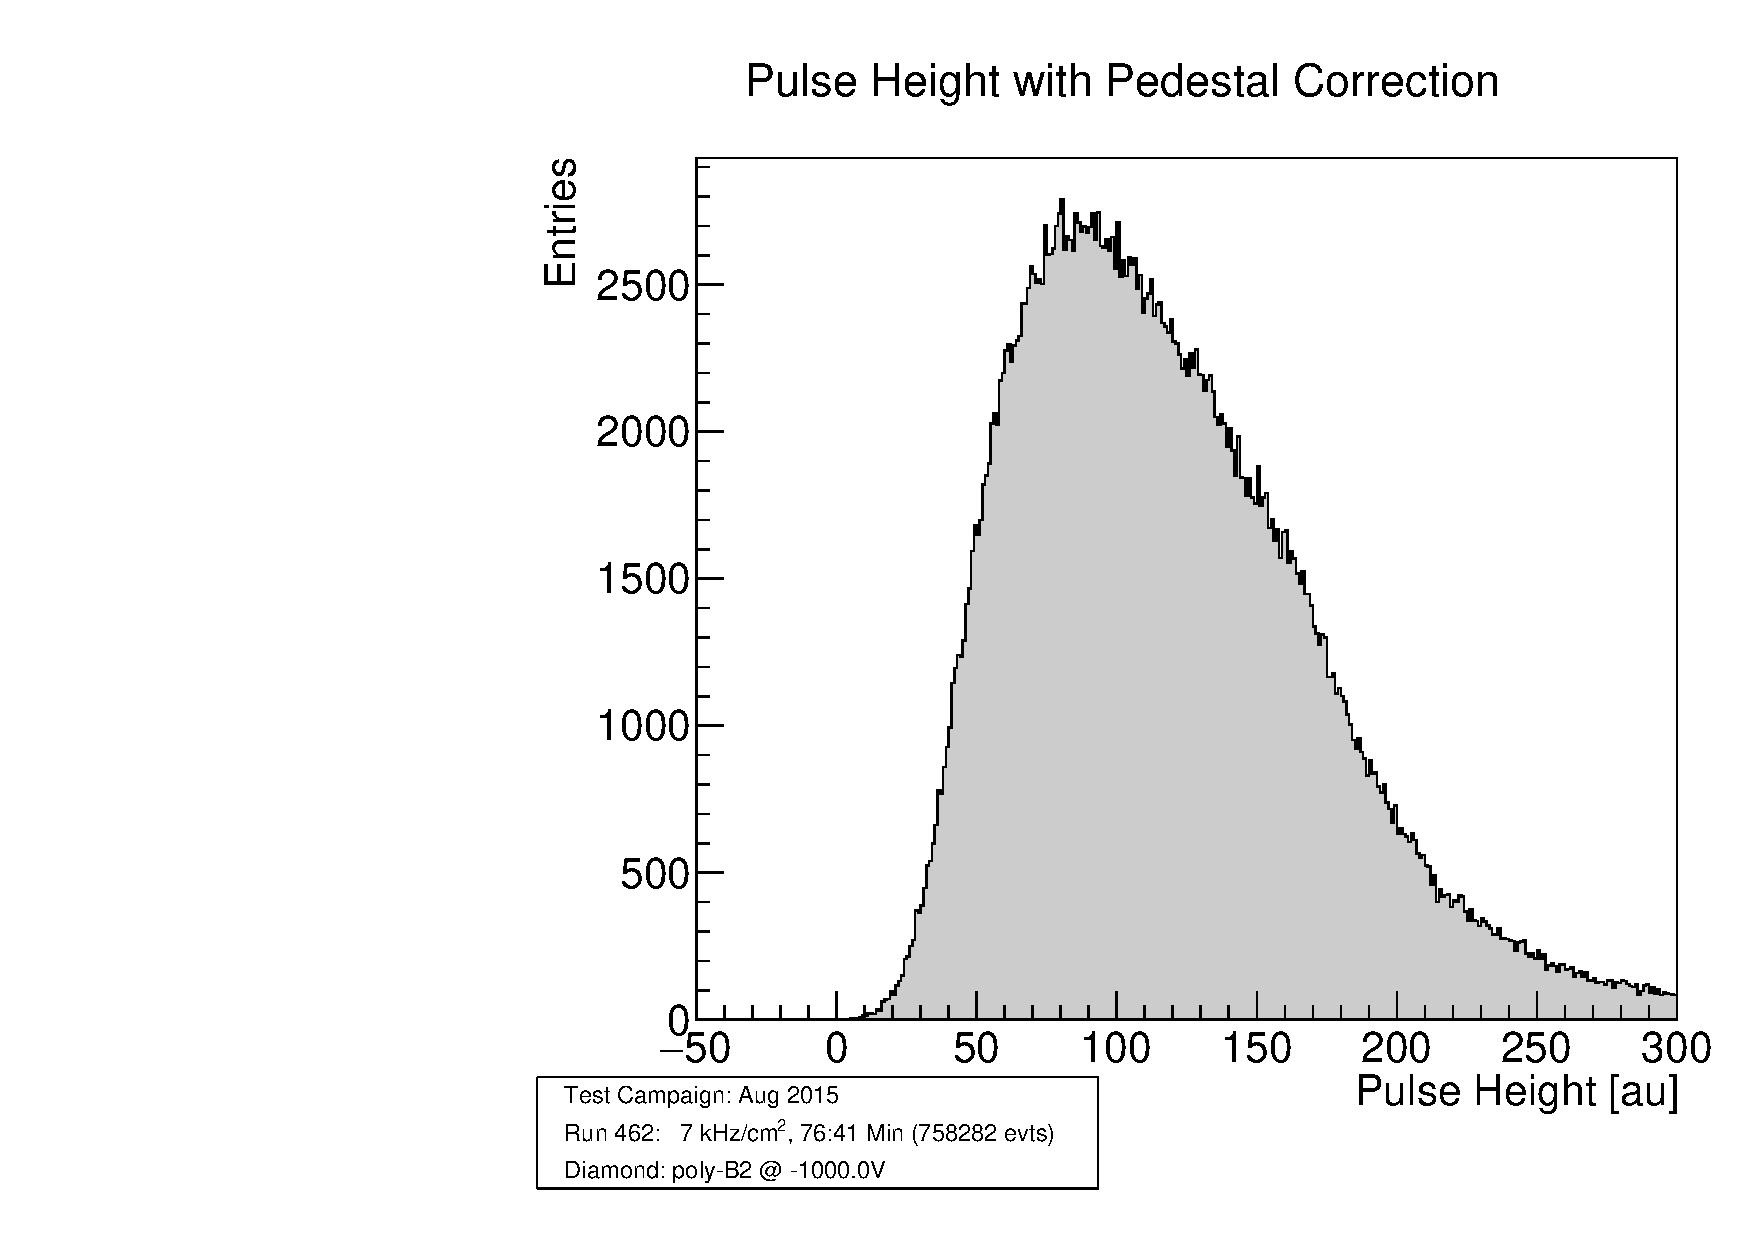
\includegraphics[angle=270, width=3.1cm]{SD462}\\
		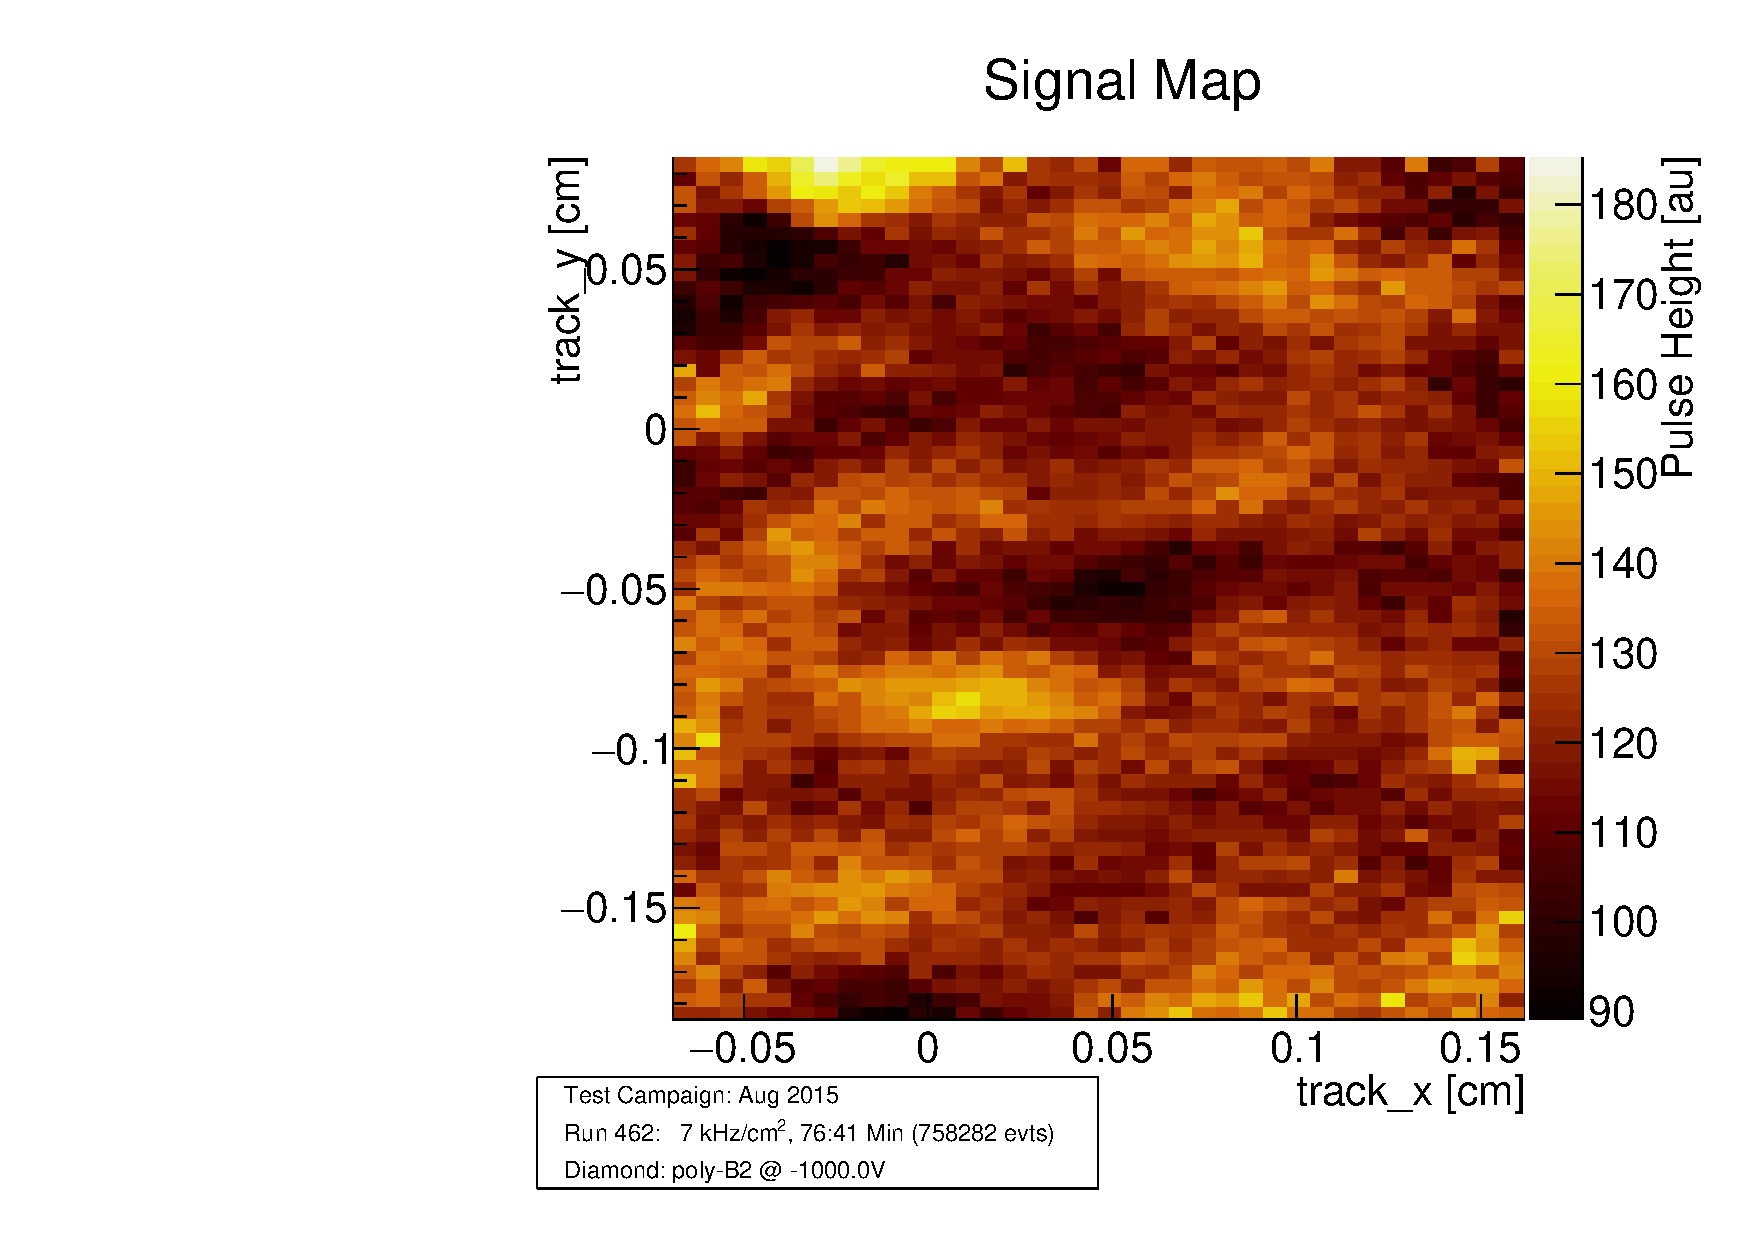
\includegraphics[angle=270, width=3.1cm]{SM462}
	\end{minipage}
	\hspace*{2pt}
	\begin{minipage}{3.1cm}
		\centering
		October 2015 - \SI[exponent-product = \cdot]{5e14}{n/cm^{2}}
		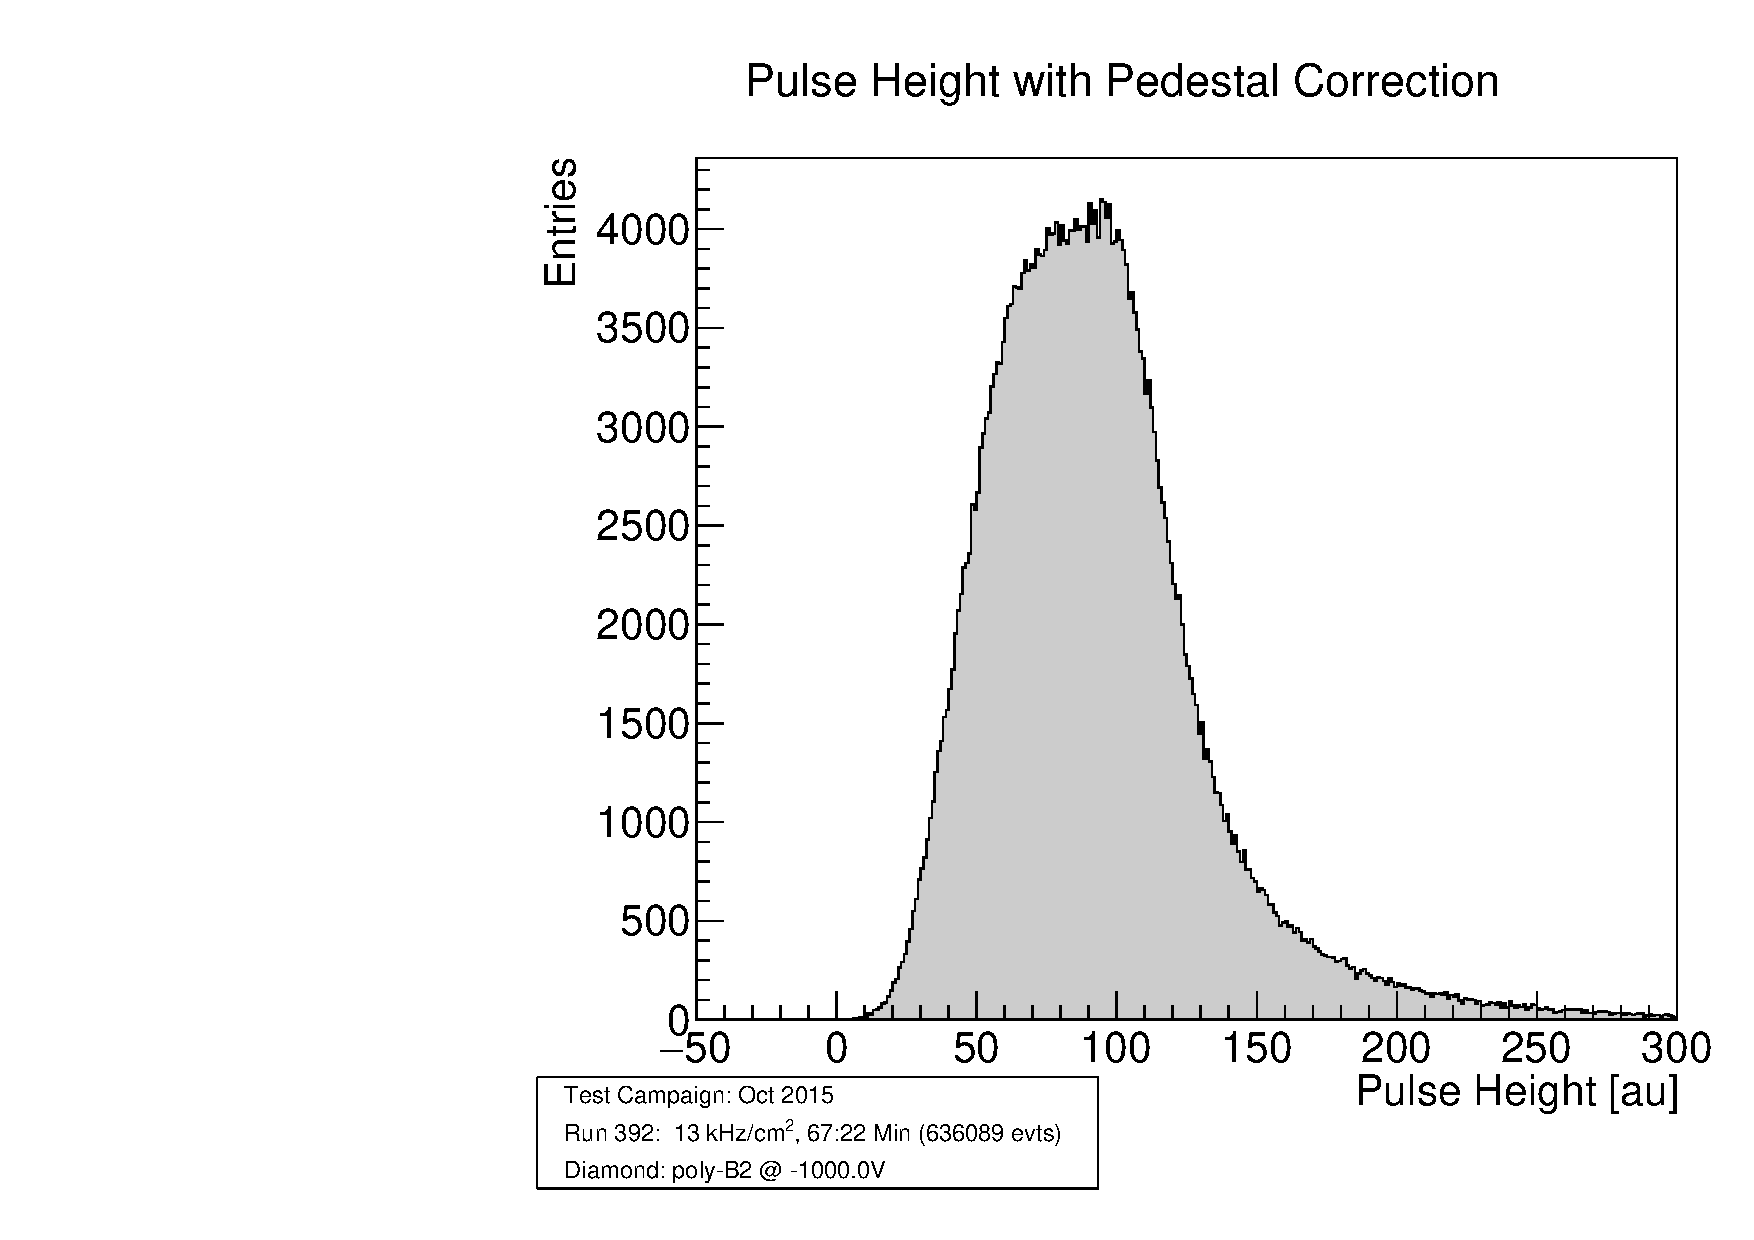
\includegraphics[angle=270, width=3.1cm]{SD392}\\
		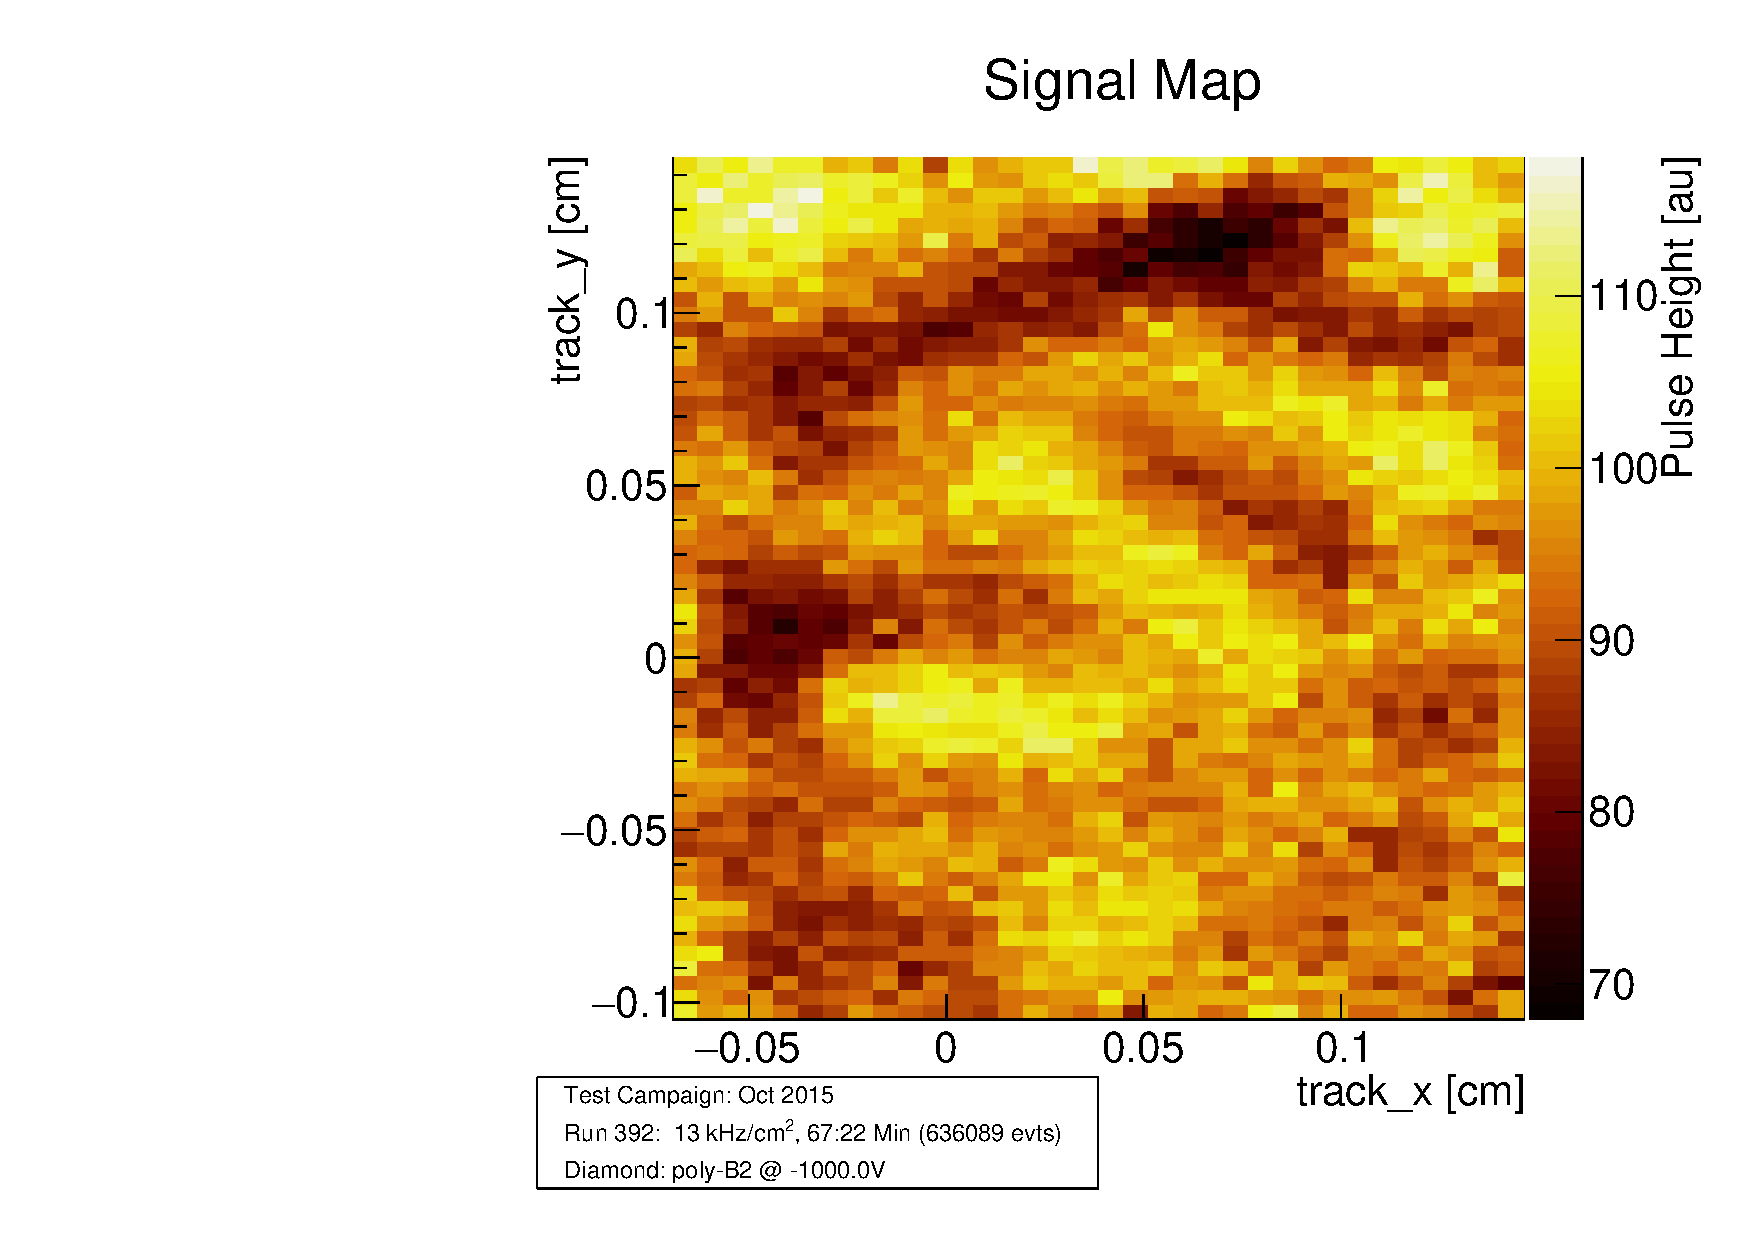
\includegraphics[angle=270, width=3.1cm]{SM392}
	\end{minipage}
	\hspace*{2pt}
	\begin{minipage}{3.1cm}
		\centering
		August 2016 - \SI[exponent-product = \cdot]{1e15}{n/cm^{2}}
		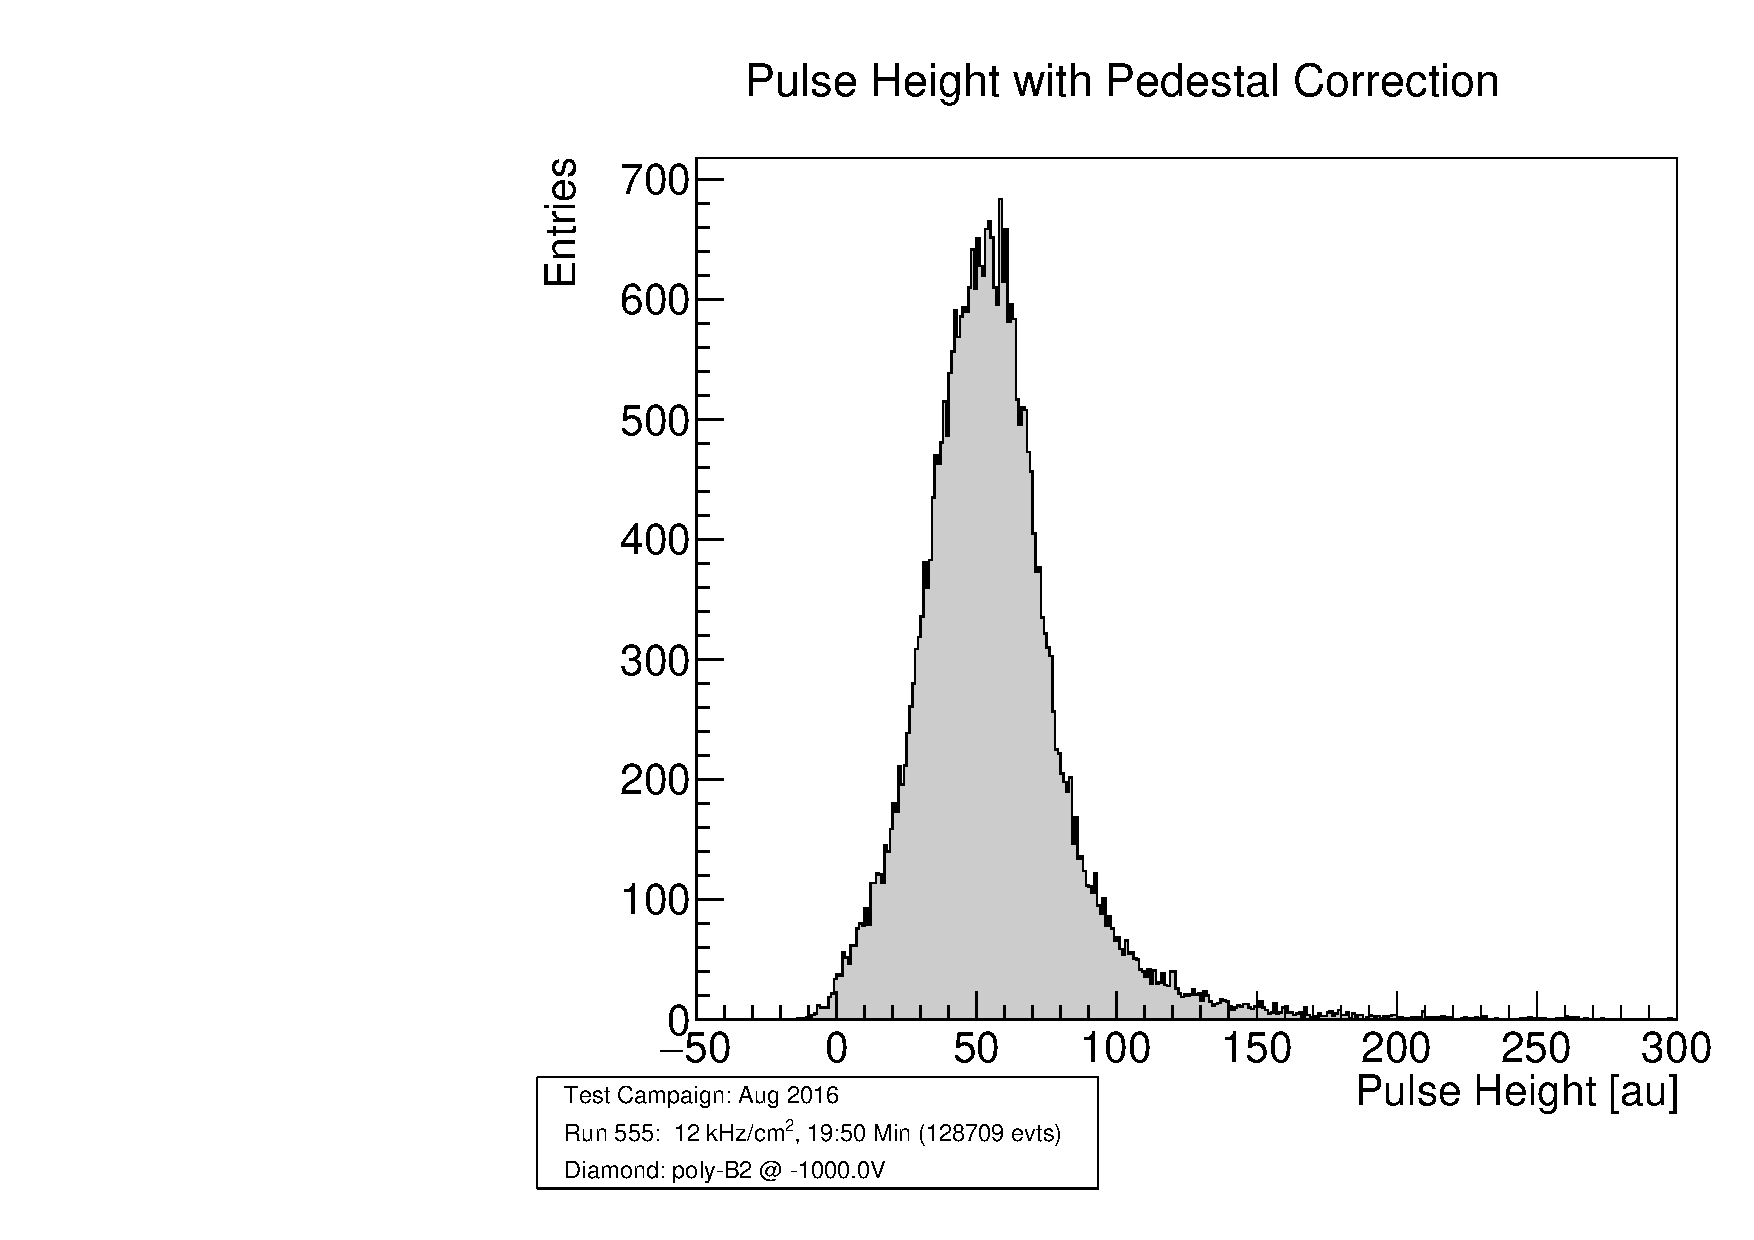
\includegraphics[angle=270, width=3.1cm]{SD555}\\
		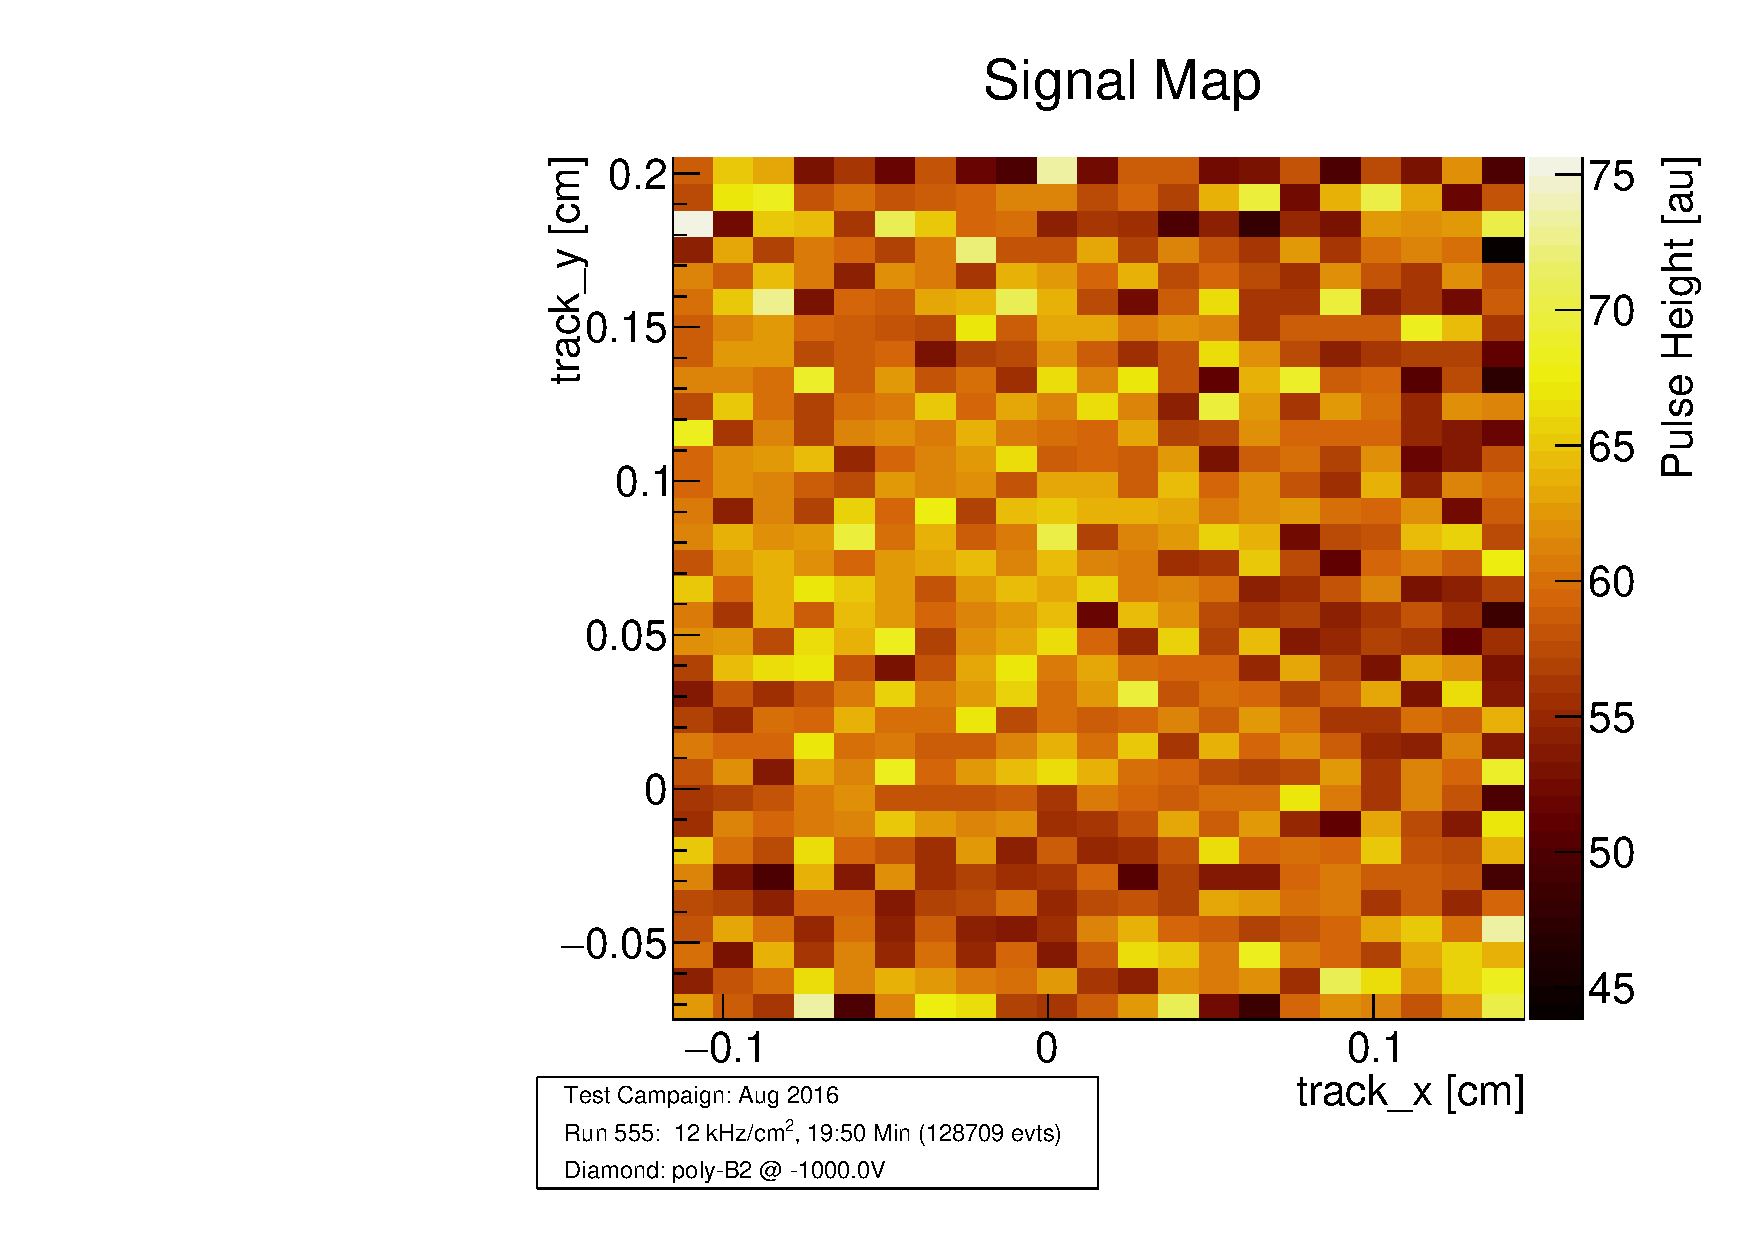
\includegraphics[angle=270, width=3.1cm]{SM555}
	\end{minipage}\s
\end{frame}
% ============================
\subsection{II6-94 and II6-95 (II-VI - poly crystal}
\begin{frame}
	\frametitle{II6-94 and II6-95 @ $-$\SI{1000}{V}}
	\centering
	\begin{minipage}{2.7cm}
		\centering
		II6-94 - \\unirradiated
		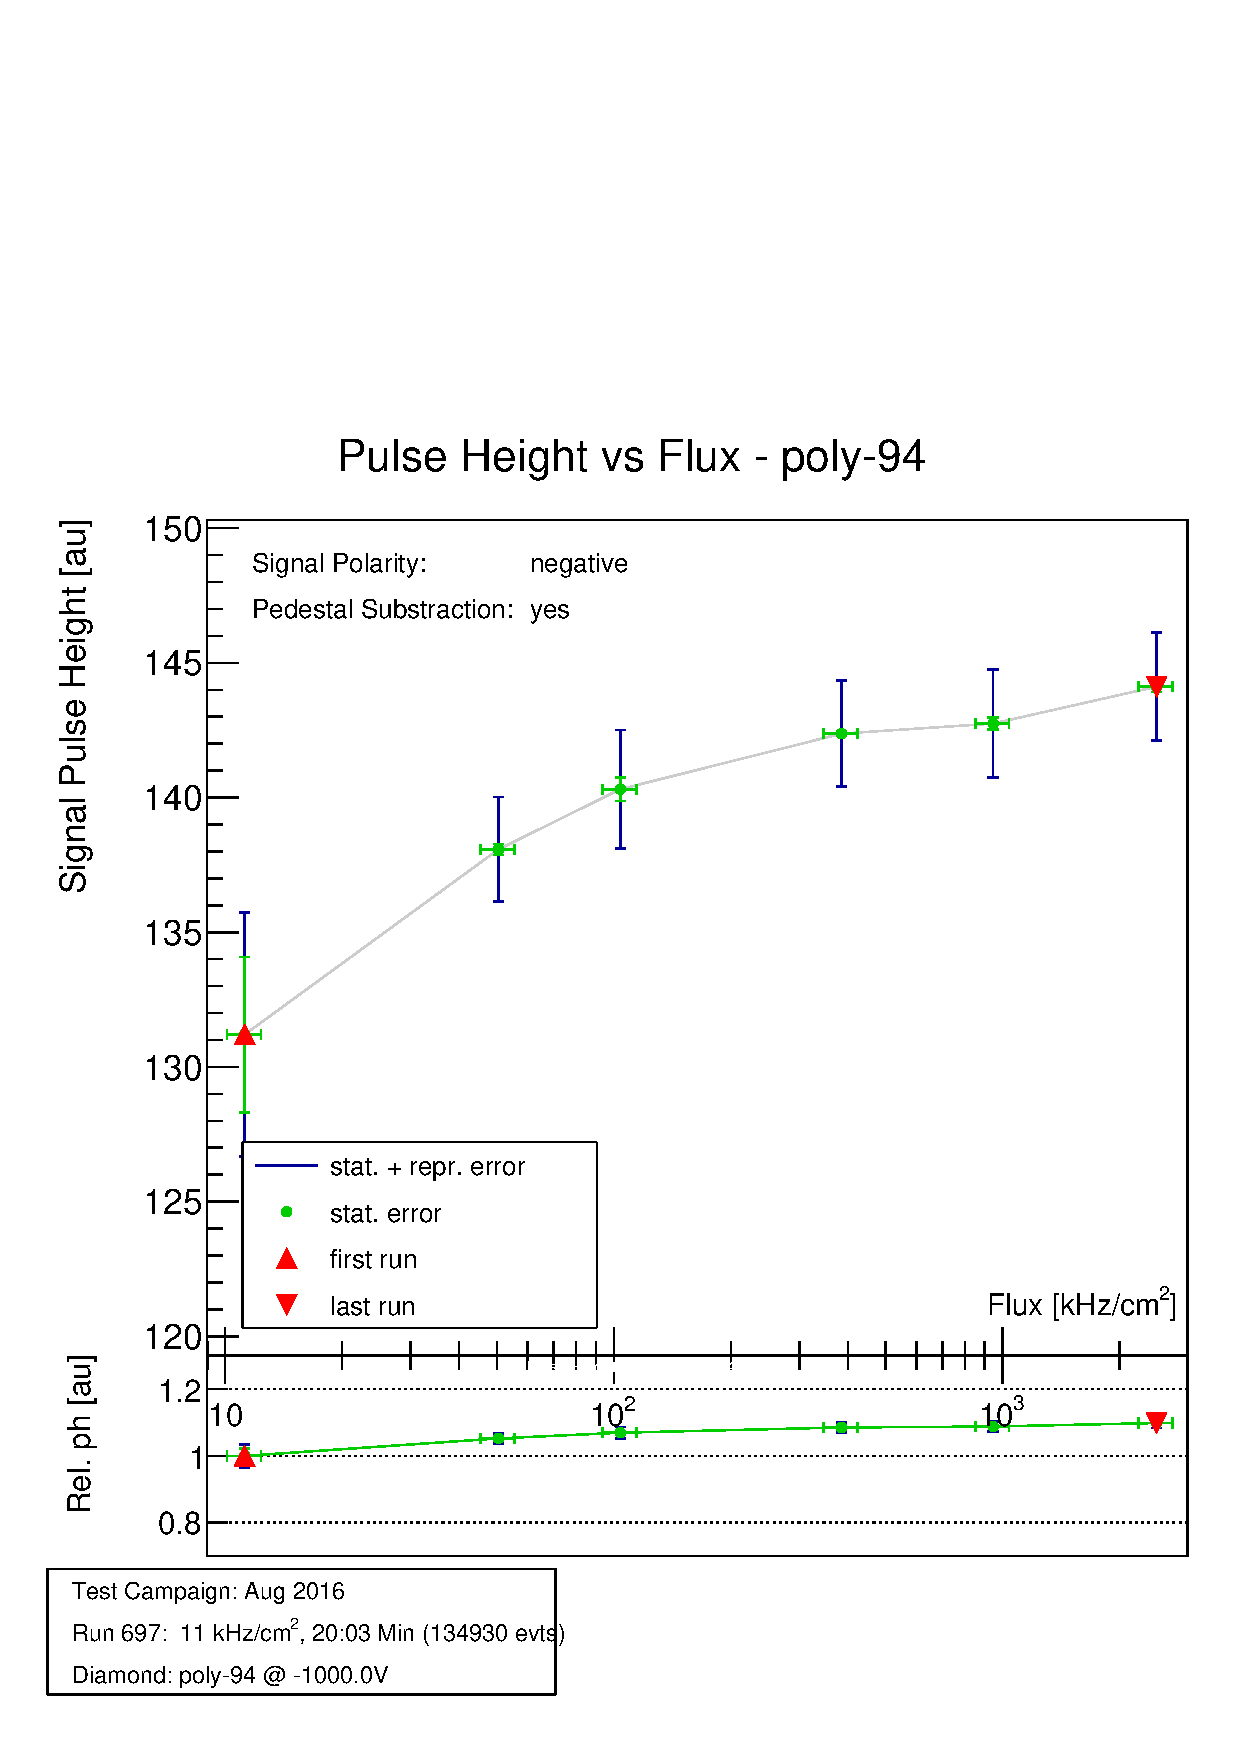
\includegraphics[width=2.7cm]{CPH1608_14_1}\\
		noise $\upsigma\approx$ \SI{5.7}{au}\\
		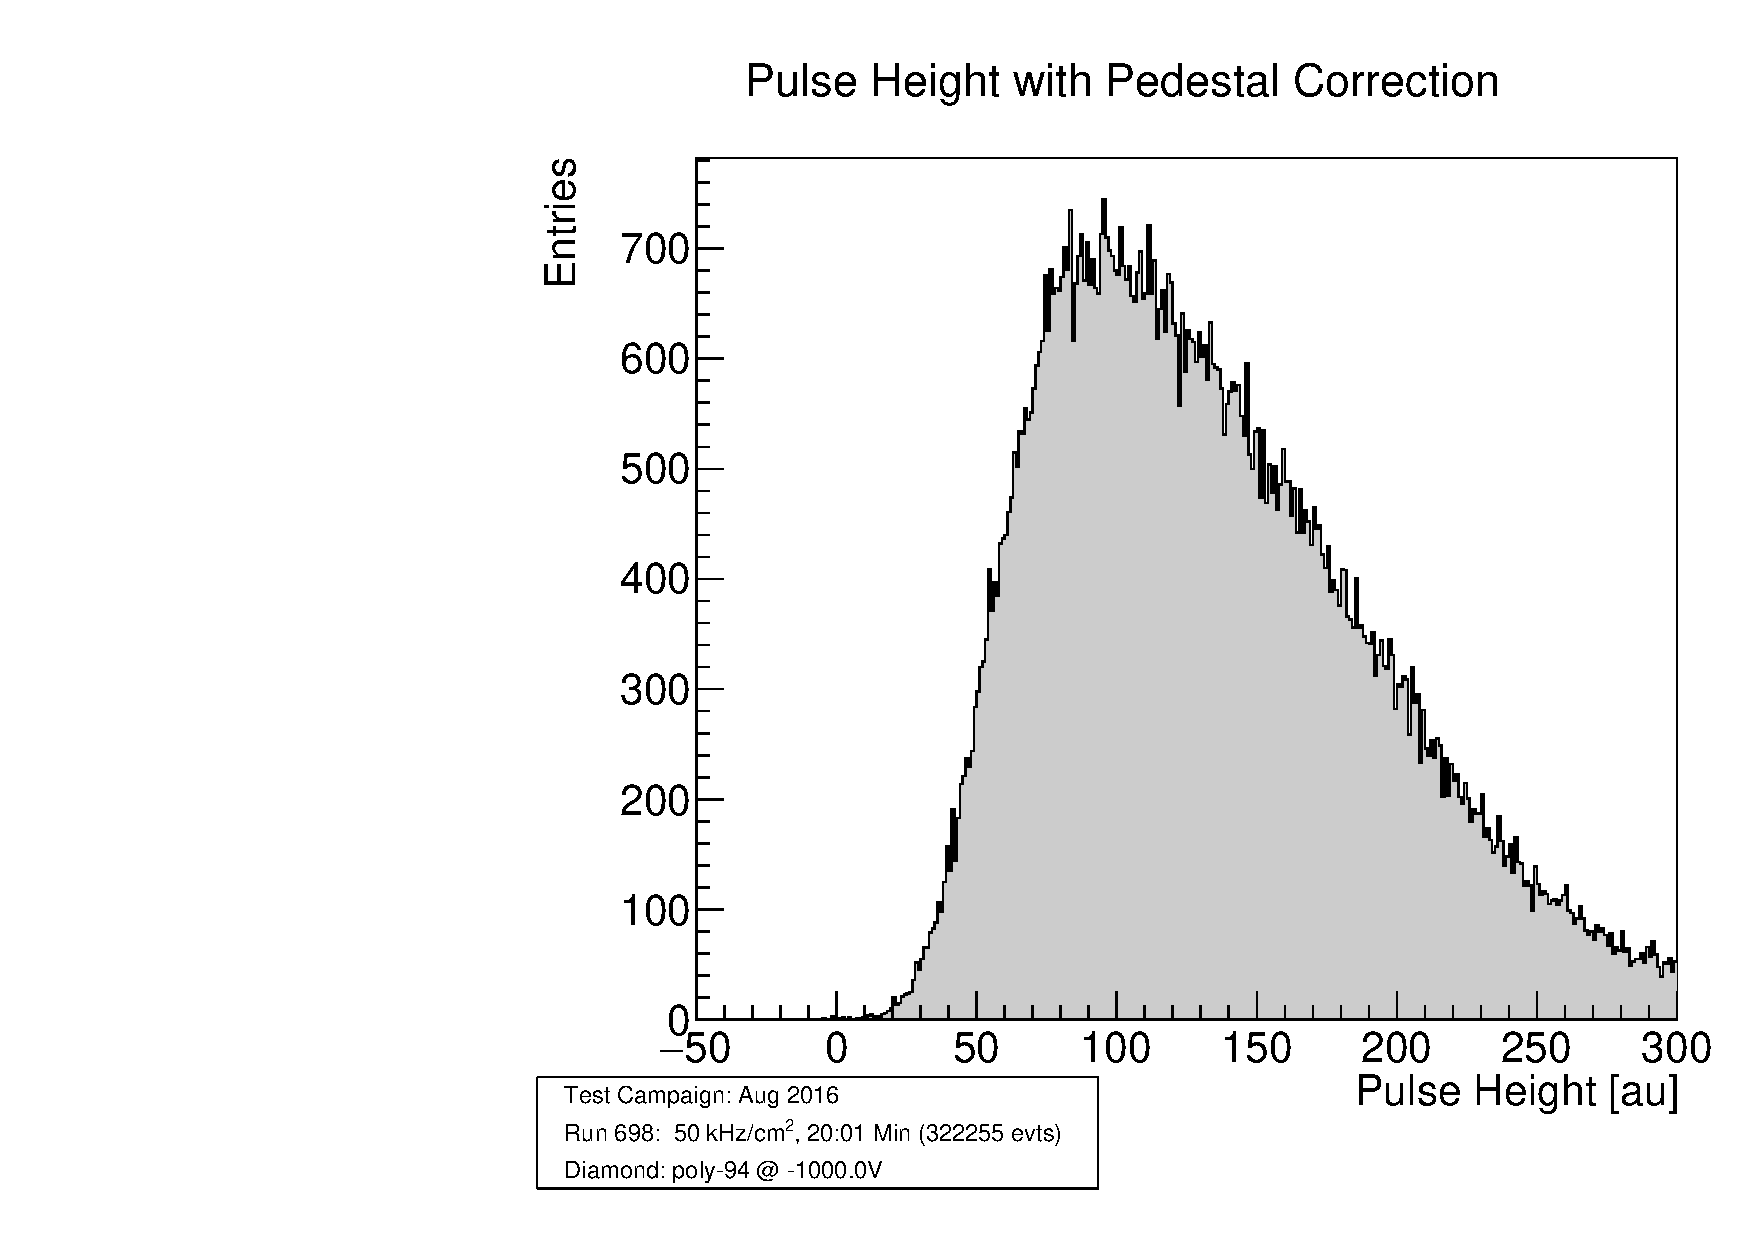
\includegraphics[angle=270, width=2.7cm]{SD698}
	\end{minipage}
	\hspace*{2pt}
	\begin{minipage}{2.7cm}
		\centering
		II6-95 - \SI[exponent-product = \cdot]{5e14}{n/cm^{2}}
		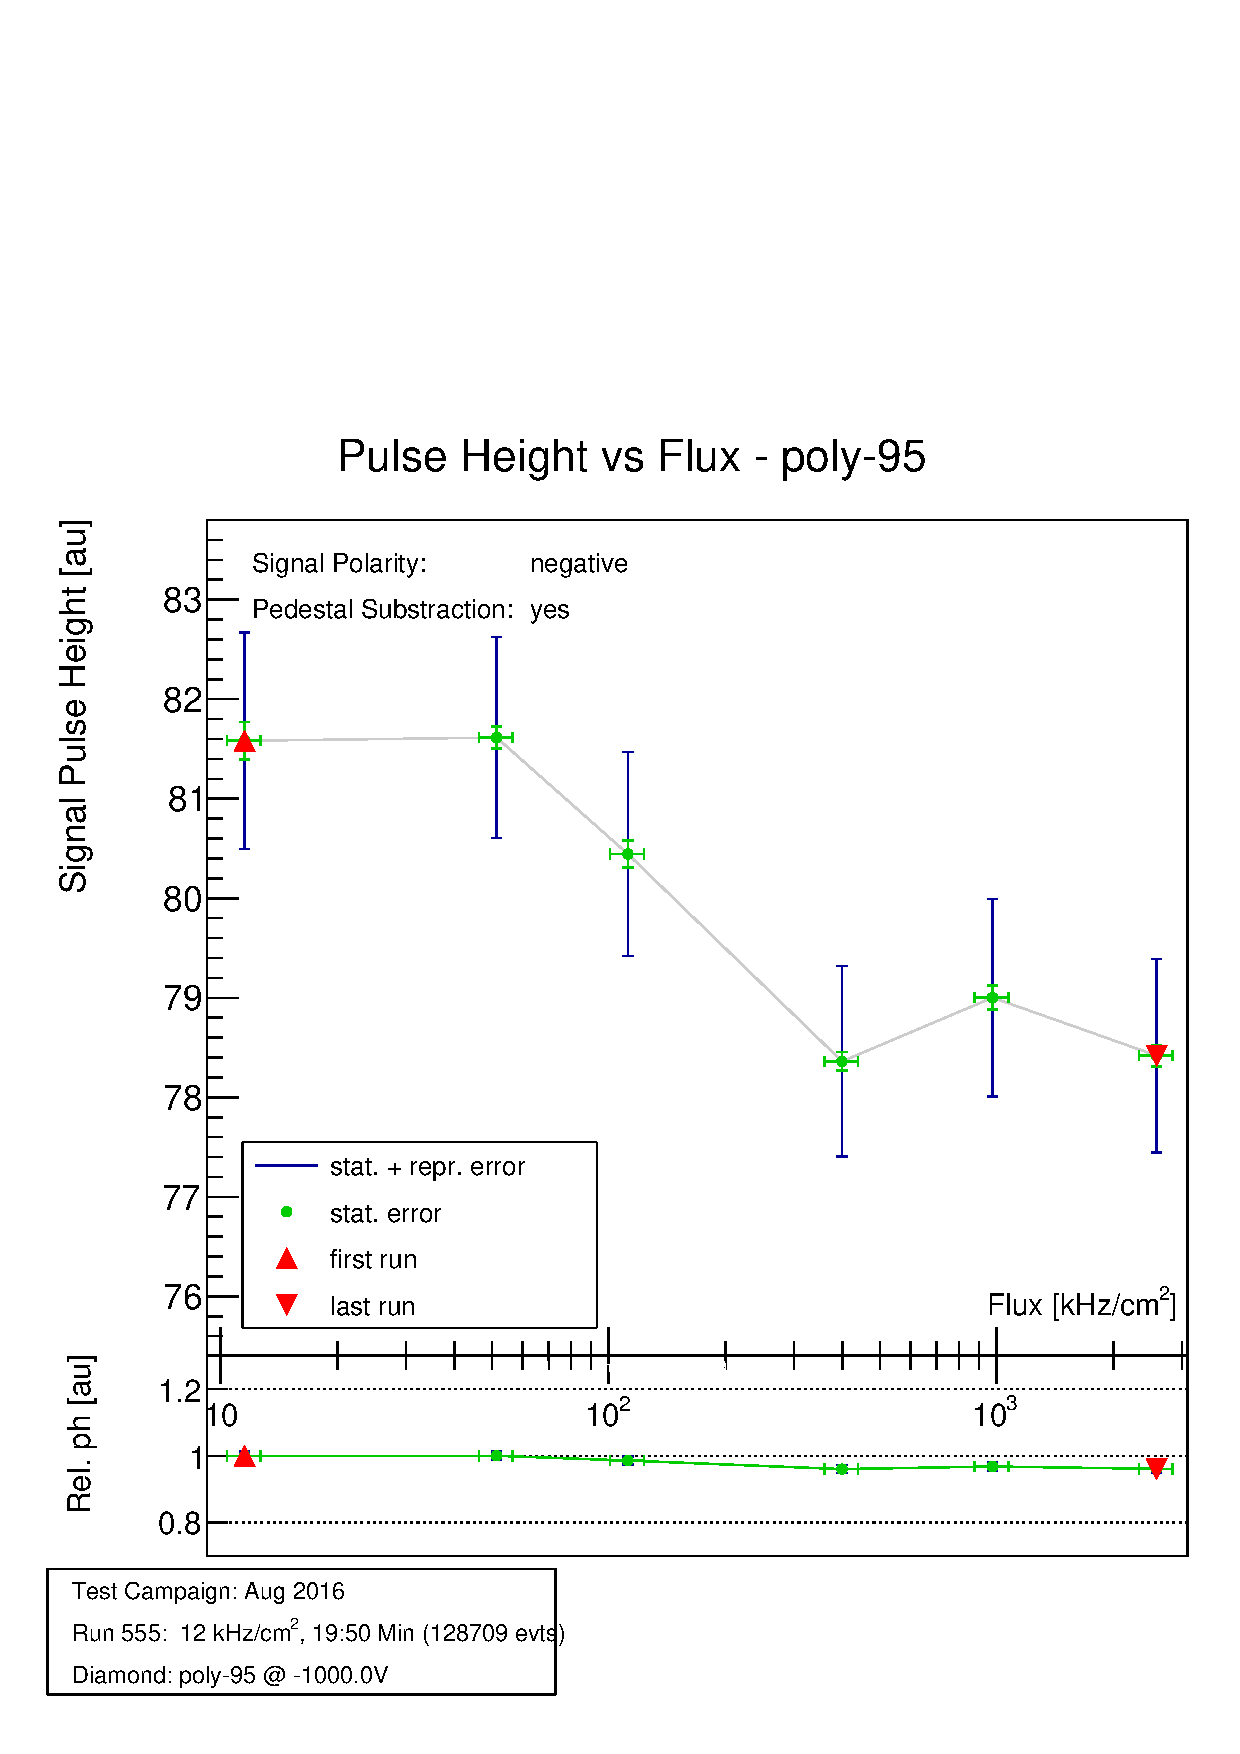
\includegraphics[width=2.7cm]{CPH1608_09_1}\\
		noise $\upsigma\approx$ \SI{4.7}{au}\\
		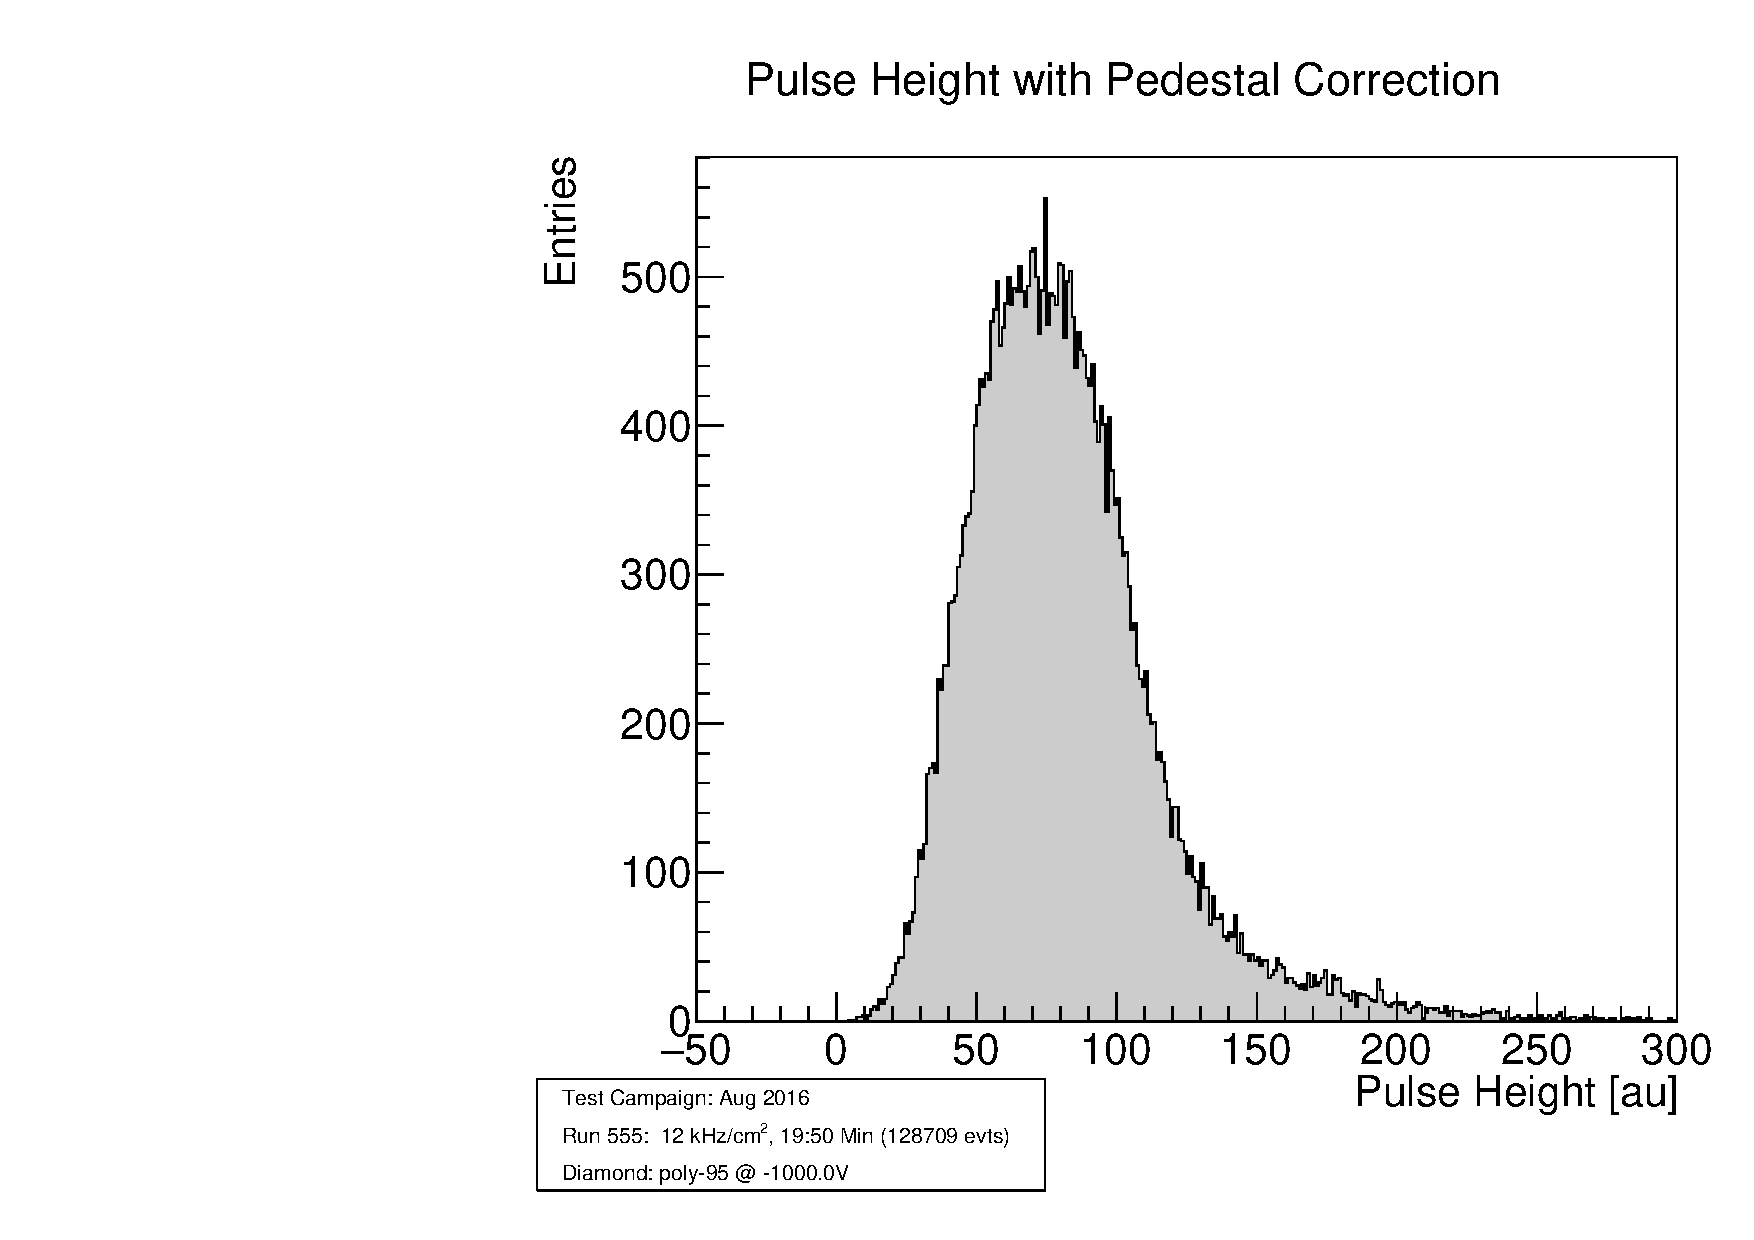
\includegraphics[angle=270, width=2.7cm]{SD555_2}
	\end{minipage}
\end{frame}
% ============================
\subsection{SiD1 (PSI - silicon diode}
\begin{frame}
	\frametitle{SiD1}
	\def \sp {4.2cm}
	\begin{minipage}{5.5cm}
		\centering
		Signal Pulse Height
		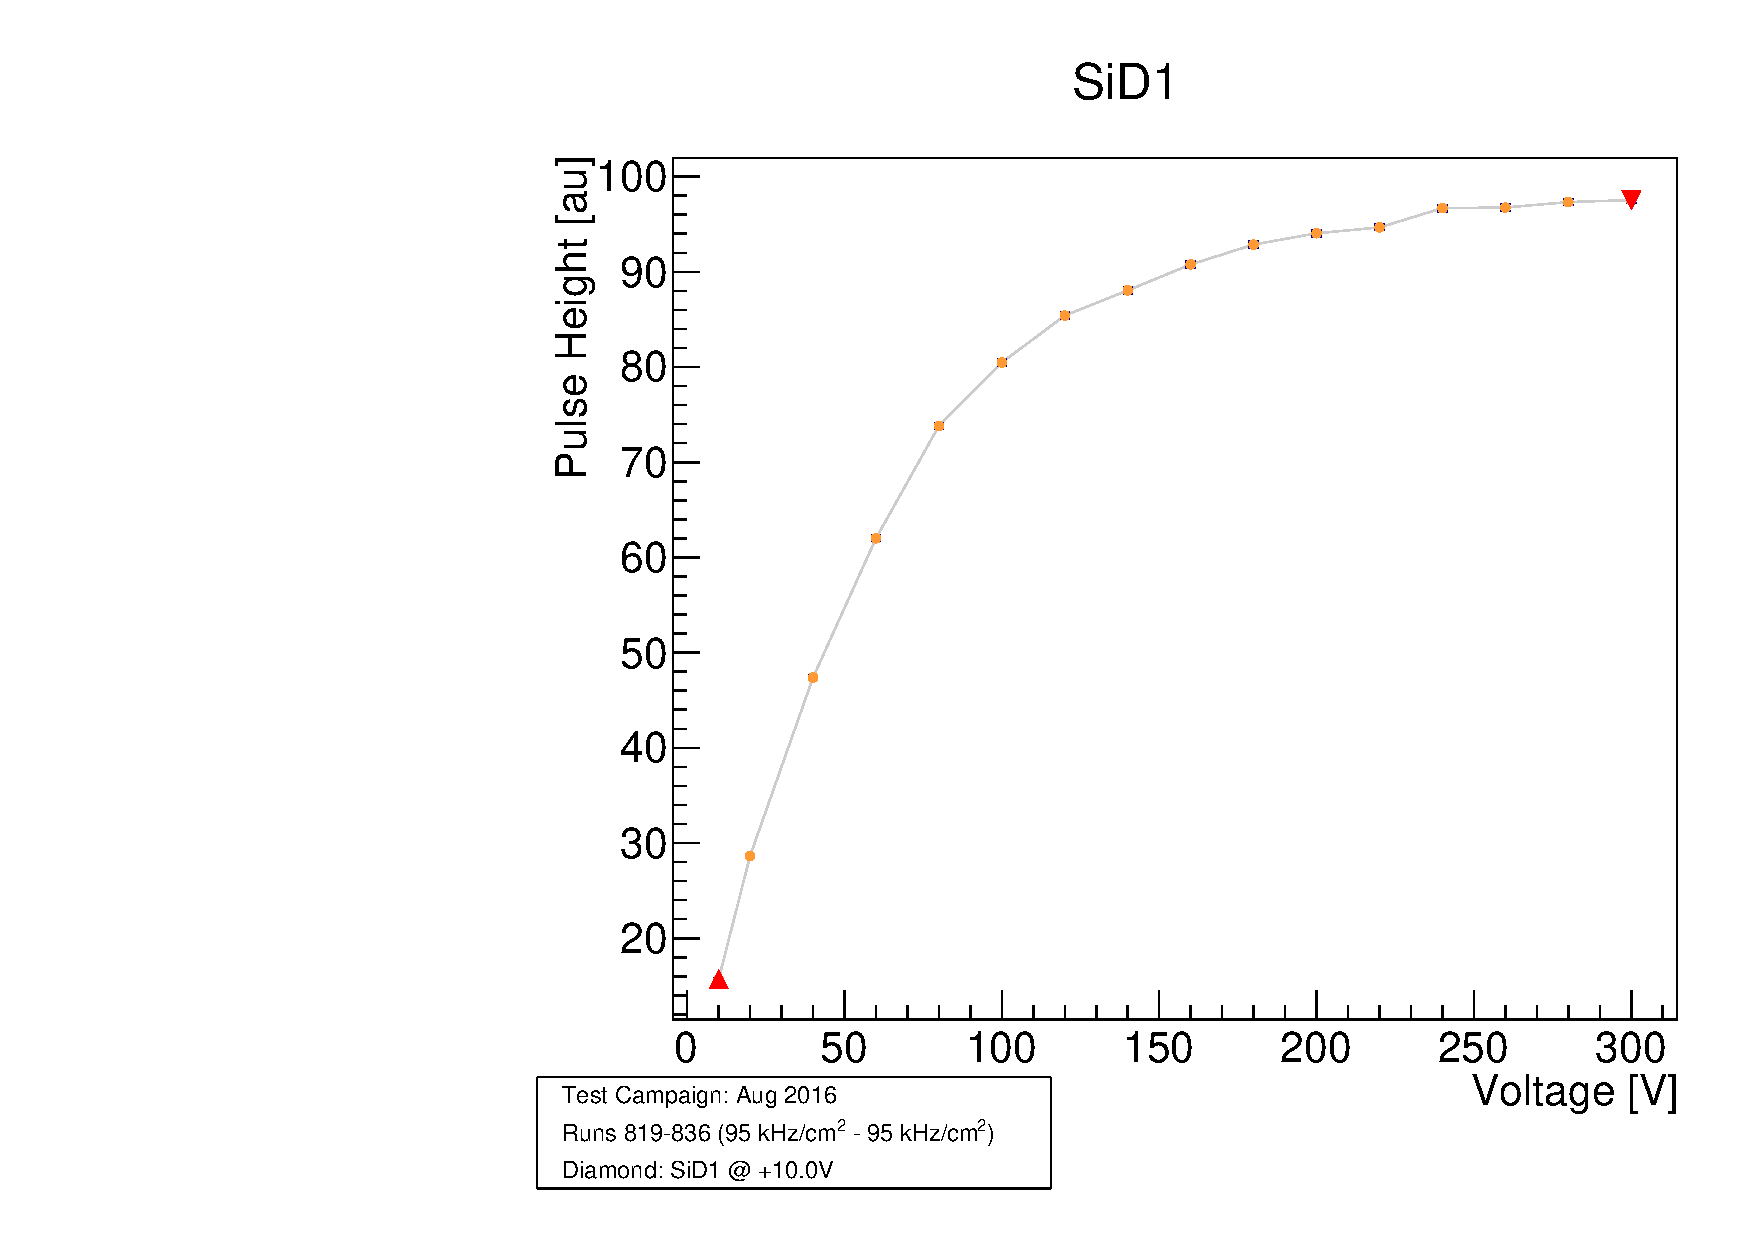
\includegraphics[angle=270, width=\sp]{PVS19}
	\end{minipage}
	\hspace*{2pt}
	\begin{minipage}{5.5cm}
		\centering
		Pulser Pulse Height
		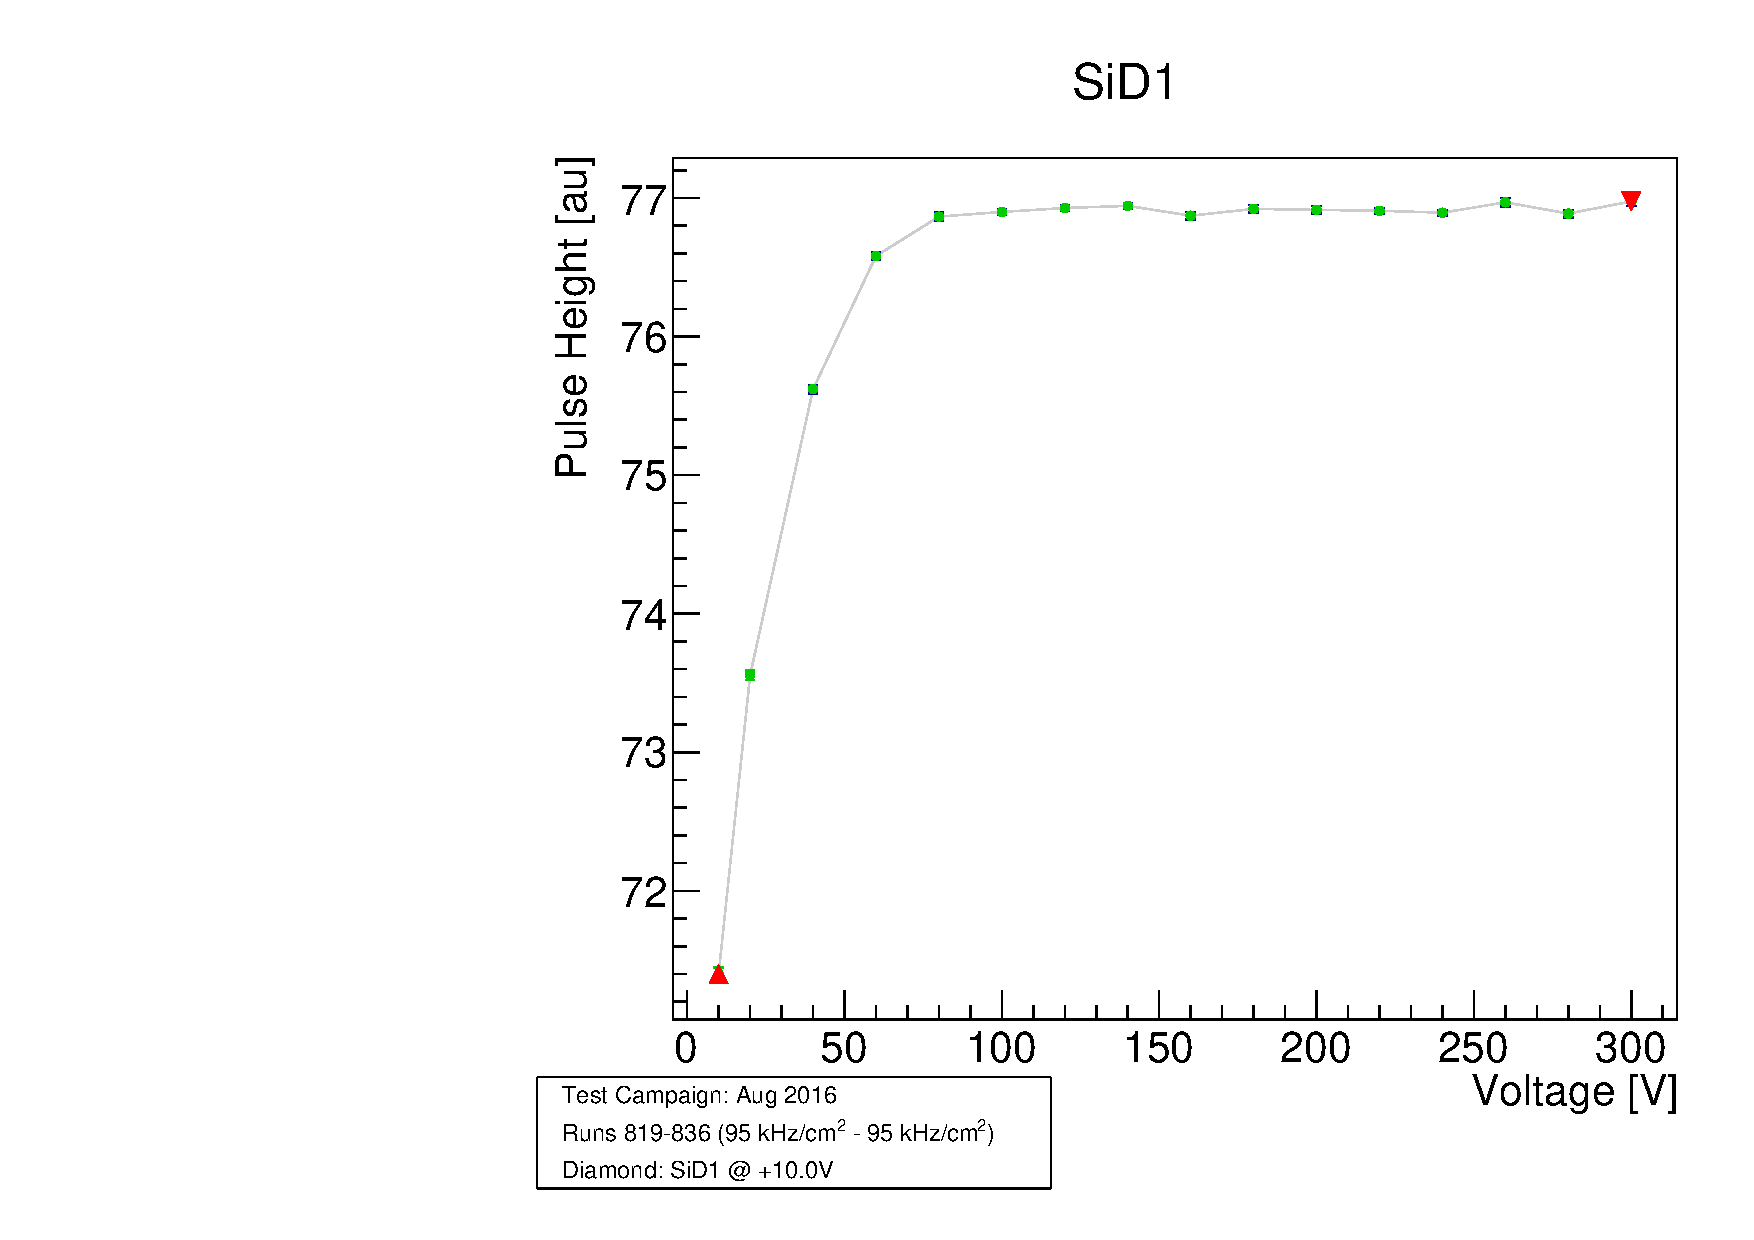
\includegraphics[angle=270, width=\sp]{SVC19}
	\end{minipage}\s
	\begin{itemize}
		\item signal supposed to saturate at \SI{\approx80}{V}
		\item pulser saturates at expected value
		\item try to use it as calibration to extract CCD of diamonds did not succeed (deviation of \SI{\approx15}{\%})
	\end{itemize}
\end{frame}
% new frame =======================
\begin{frame}
	\def \sp {5cm}
	\begin{minipage}{5.5cm}
		\centering
		Signal Map
		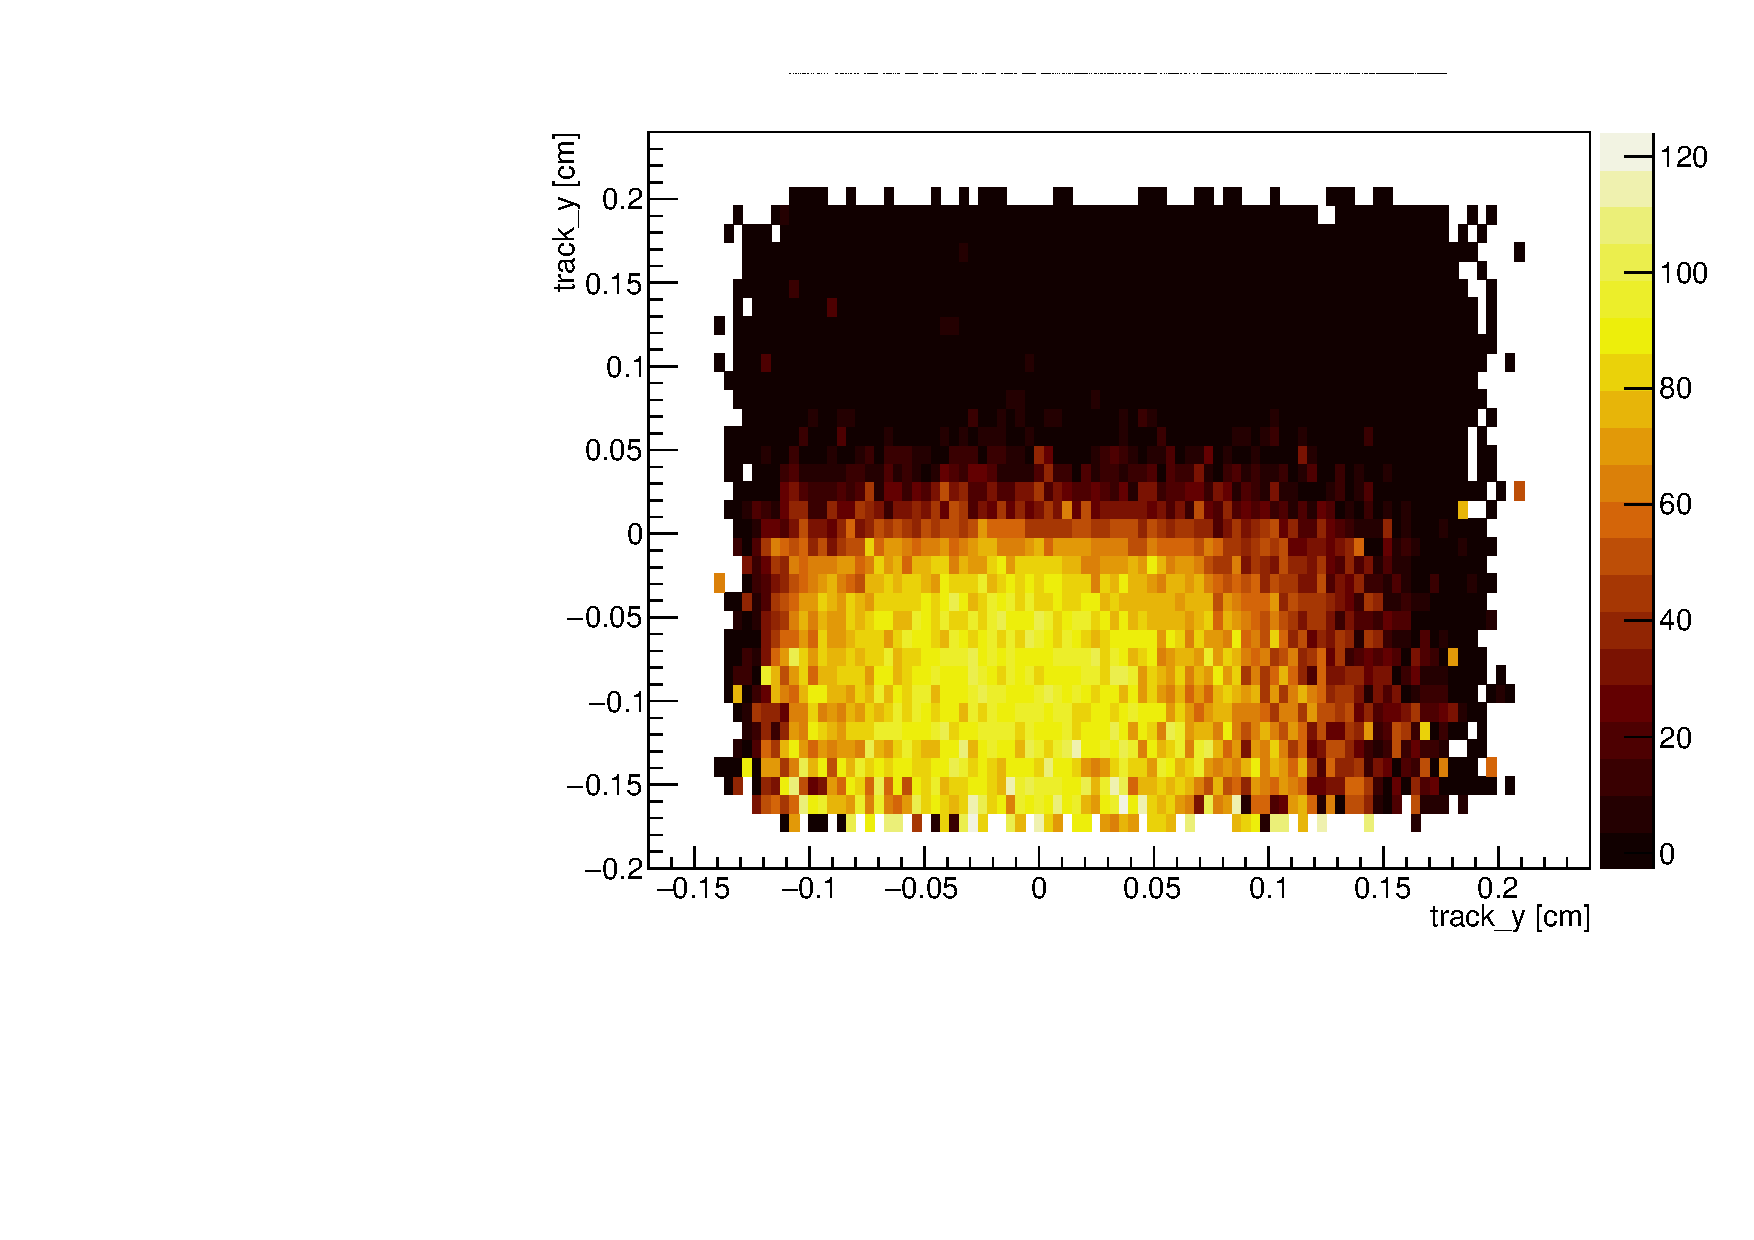
\includegraphics[angle=270, width=\sp]{SiD1SM}
	\end{minipage}
	\hspace*{2pt}
	\begin{minipage}{5.5cm}
		\centering
		Rate Scan
		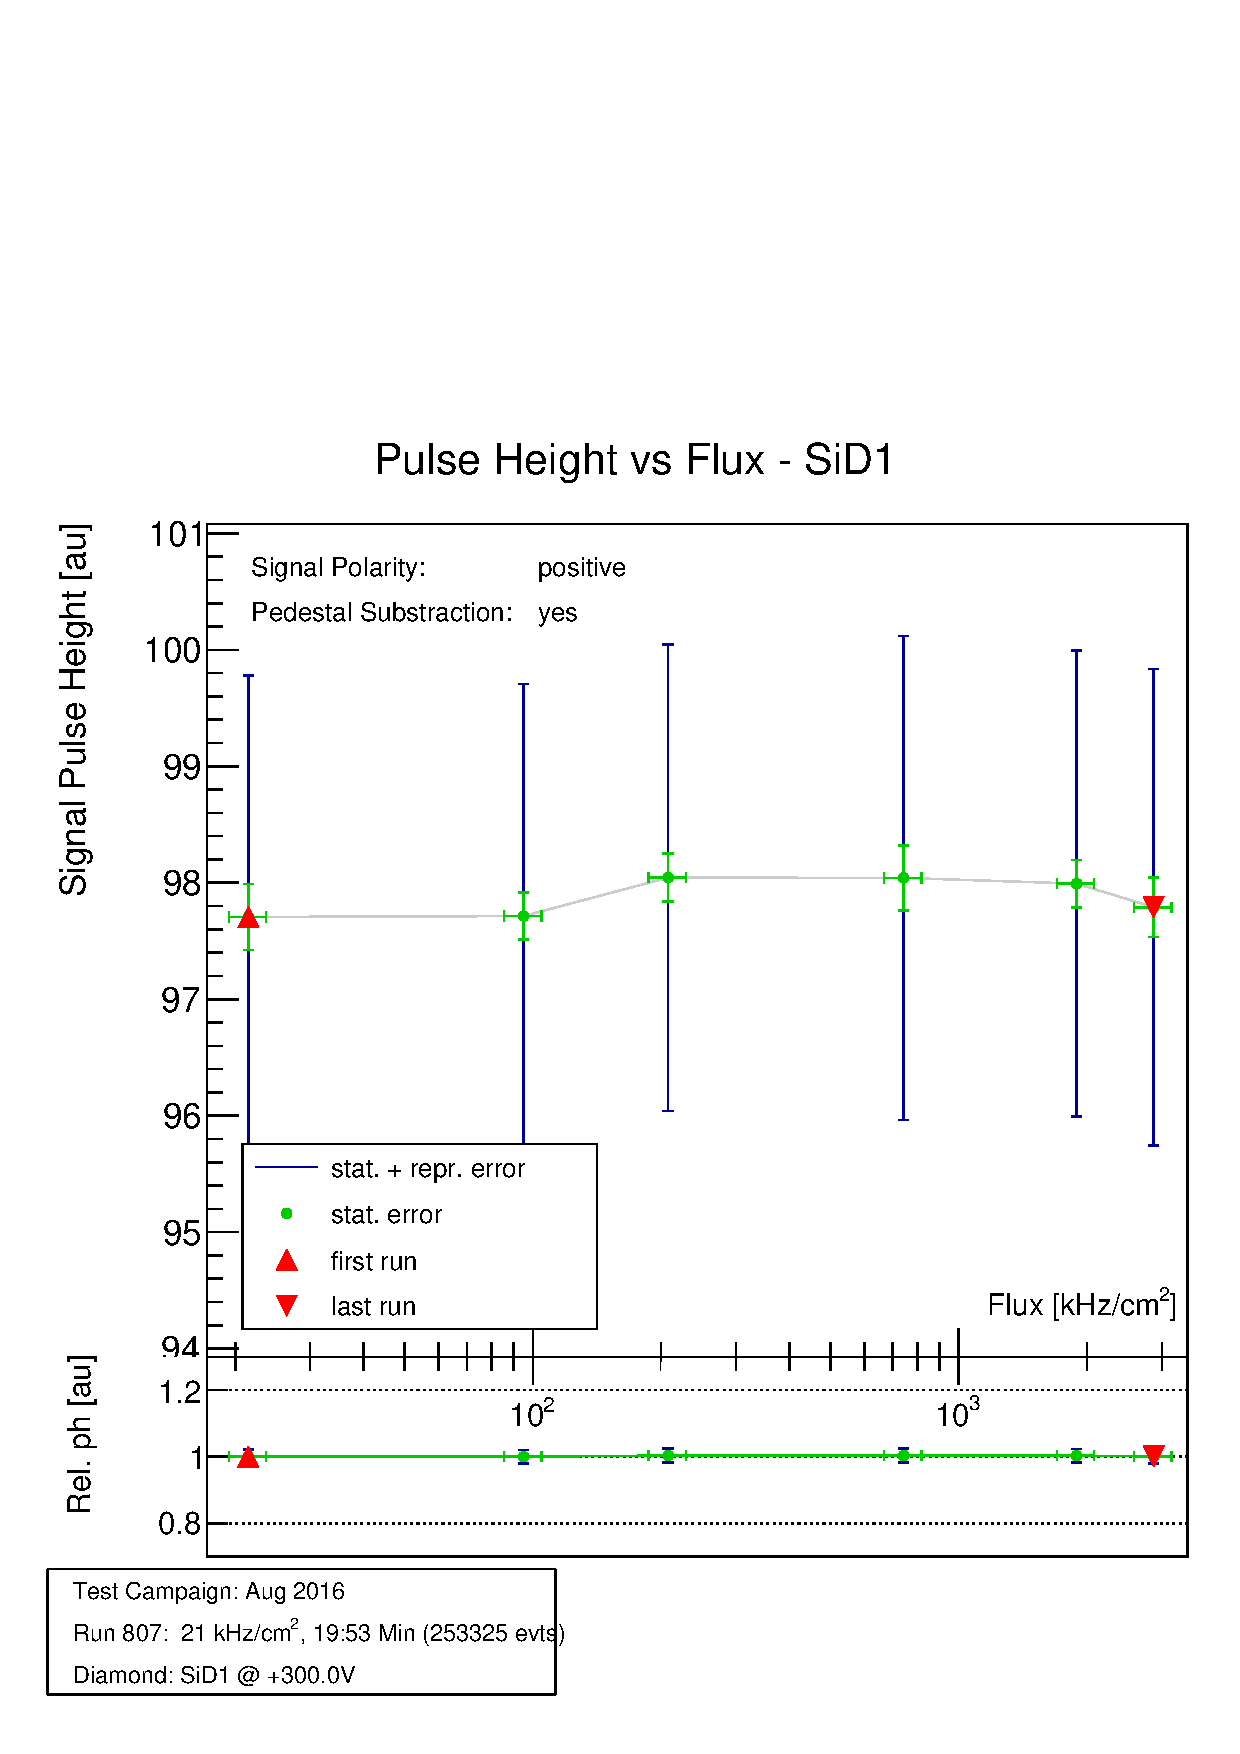
\includegraphics[width=\sp]{CPH1608_18_1_2}
	\end{minipage}\s
	\begin{itemize}
		\item pulse height very flat with rate $\rightarrow$ no rate dependence
	\end{itemize}
\end{frame}
% END 
% ====================================================================================
% CONCLUSION
% ====================================================================================
\section{Conclusion}
% ============================
\begin{frame}
	\frametitle{Conclusion}
	\begin{itemize}
		\setlength{\itemsep}{\fill}
		\item very good timing resolution with scintillator allows for precise integration and separation of the signals
		\item tests in August 2016 are compatible with the beam test before
		\item unirradiated single crystal shows almost no rate dependence
		\begin{itemize}
			\item good reference
		\end{itemize}
		\item behaviour of silicon diode not yet understood
		\begin{itemize}
			\item yet very stable with rate
		\end{itemize}
	\end{itemize}
\end{frame}
% ====================================================================================
% OUTLOOK
% ====================================================================================
\section{Outlook}
% ============================
\begin{frame}
	\frametitle{Outlook}
	\begin{itemize}
		\setlength{\itemsep}{\fill}
		\item irradiate II6-B2 further 
		\item find other stable poly-crystalline diamonds
		\item investigate behaviour of silicon diode
		\item build and test further silicon diode
	\end{itemize}
\end{frame}
% ============================
% DOCUMENT END
\end{document}

